\newcommand*{\ATLASLATEXPATH}{latex/}
\documentclass[UKenglish,texlive=2011,PAPER]{\ATLASLATEXPATH atlasdoc}
% The following command is needed by arXiv to ensure use of pdflatex.
% It should be included in the first 5 lines of the preamble.
% \pdfoutput=1
%  cernpreprint          Create front page for a CERN preprint.
%                        See atlas-preprint-cover.tex for a list of variables that should be defined.
%  txfonts=true|false    Use txfonts rather than the default newtx - needed for arXiv submission.
\usepackage[subcaption]{\ATLASLATEXPATH atlaspackage}
\usepackage{\ATLASLATEXPATH atlasprocess}
\usepackage{\ATLASLATEXPATH atlasmisc}
\usepackage{\ATLASLATEXPATH atlasbiblatex}
\usepackage{\ATLASLATEXPATH atlascontribute}
\usepackage{\ATLASLATEXPATH atlasphysics}
\usepackage{\ATLASLATEXPATH atlasbsm}

\addbibresource{newSUSYRefs.bib}
\addbibresource{ss3l2015pub.bib}
\addbibresource{bibtex/bib/ATLAS.bib}
\addbibresource{bibtex/bib/PubNotes.bib}
\addbibresource{bibtex/bib/ConfNotes.bib}

\graphicspath{{logos/}{FIGURES/}}

\usepackage{ss3l2015pub-defs}
\usepackage[normalem]{ulem}
\usepackage{xparse}
\captionsetup[subfigure]{labelformat=simple}
\renewcommand*{\thesubfigure}{(\alph{subfigure})}

%-------------------------------------------------------------------------------
% This file contains the title, author and abstract.
% It also contains all relevant document numbers used by the different cover pages.
%-------------------------------------------------------------------------------

% Title
\AtlasTitle{Search for supersymmetry at $\sqrt{s}=13$~TeV in final states with jets and two same-sign leptons or three leptons with the ATLAS detector}

% Author - this does not work with revtex (add it after \begin{document})
\author{The ATLAS Collaboration}

% Authors and list of contributors to the analysis
% \AtlasAuthorContributor also adds the name to the author list
% Include package latex/atlascontribute to use this
% Use authblk package if there are multiple authors, which is included by latex/atlascontribute
% \usepackage{authblk}
% \renewcommand\Authands{, } % avoid ``. and'' for last author
% \renewcommand\Affilfont{\itshape\small} % affiliation formatting
% \AtlasAuthorContributor{First AtlasAuthorContributor}{a}{Author's contribution.}
% \AtlasAuthorContributor{Second AtlasAuthorContributor}{b}{Author's contribution.}
% \AtlasAuthorContributor{Third AtlasAuthorContributor}{a}{Author's contribution.}
% \AtlasContributor{Fourth AtlasContributor}{Contribution to the analysis.}
% \author[a]{First Author}
% \author[a]{Second Author}
% \author[b]{Third Author}
% \affil[a]{One Institution}
% \affil[b]{Another Institution}

% If a special author list should be indicated via a link use the following code:
% Include the two lines below if you do not use atlasstyle:
% \usepackage[marginal,hang]{footmisc}
% \setlength{\footnotemargin}{0.5em}
% Use the following lines in all cases:
% \usepackage{authblk}
% \author{The ATLAS Collaboration%
% \thanks{The full author list can be found at:\newline
%   \url{https://atlas.web.cern.ch/Atlas/PUBNOTES/ATL-PHYS-PUB-2014-007/authorlist.pdf}}
% }

\AtlasVersion{3.2}

% ATLAS reference code, to help ATLAS members to locate the paper
\AtlasRefCode{SUSY-2015-09}
%\AtlasRefCode{ATLAS-CONF-2015-078}


% CERN preprint number
% \PreprintIdNumber{CERN-PH-2014-XX}

% ATLAS date - arXiv submission; to be filled in by the Physics Office
% \AtlasDate{\today}

% arXiv identifier
% \arXivId{14XX.YYYY}

% HepData record
% \HepDataRecord{ZZZZZZZZ}

% Submission journal and final reference
\AtlasJournal{Eur.\ Phys.\ J.\ C}
% \AtlasJournalRef{\PLB 789 (2014) 123}
% \AtlasDOI{}

% Abstract - % directly after { is important for correct indentation
\AtlasAbstract{A search for strongly produced supersymmetric particles is conducted using signatures involving multiple energetic jets and either two isolated leptons ($e$ or $\mu$) with the same electric charge or at least three isolated leptons. The search also utilises $b$-tagged jets, missing transverse momentum and other observables to extend its sensitivity. The analysis uses a data sample of proton--proton collisions at $\sqrt{s}= 13$~TeV recorded with the ATLAS detector at the Large Hadron Collider in 2015 corresponding to a total integrated luminosity of 3.2~fb$^{-1}$. No significant excess over the Standard Model expectation is observed.  
%and the results are interpreted in several simplified supersymmetric models extending the exclusion limits from previous searches. 
The results are interpreted in several simplified supersymmetric models and extend the exclusion limits from previous searches.
In the context of exclusive production and simplified decay modes, gluino masses are excluded at $95\%$ confidence level 
up to 1.1--1.3~TeV for light neutralinos (depending on the decay channel), 
and bottom squark masses are also excluded up to 540 GeV. 
In the former scenarios, neutralino masses are also excluded up to 550-850 GeV for gluino masses around 1 TeV. 
}

%-------------------------------------------------------------------------------
% The following information is needed for the cover page. The commands are only defined
% if you use the coverpage option in atlasdoc or use the atlascover package
%-------------------------------------------------------------------------------

% List of supporting notes  (leave as null \AtlasCoverSupportingNote{} if you want to skip this option)
\AtlasCoverSupportingNote{Supporting note}{https://cds.cern.ch/record/2052581}
% \AtlasCoverSupportingNote{Short title note 2}{https://cds.cern.ch/record/YYYYYYY}
%
% OR (the 2nd option is deprecated, especially for CONF and PUB notes)
%
% Supporting material TWiki page  (leave as null \AtlasCoverTwikiURL{} if you want to skip this option)
% \AtlasCoverTwikiURL{https://twiki.cern.ch/twiki/bin/view/Atlas/WebHome}

% Comment deadline
\AtlasCoverCommentsDeadline{February 25th, 2016}

% Analysis team members - contact editors should no longer be specified
% as there is a generic email list name for the editors
\AtlasCoverAnalysisTeam{B.~Abbott, J.-F.~Arguin, S.~Berlendis, F.~Cardillo, G.~Carrillo-Montoya, A.~Di~Simone, O.~Ducu, D. Gerbaudo, F.~Hubaut, G.~Herten, S.~Kahn, A.~Lleres, J.~Maurer, E.~Monnier, T.~Nguyen, A.~Paramonov, J.~Poveda, P.~Pralavorio, H.~Ren, O.~Rifki, Y.-T.~Shen, P.~Skubic, A.~Taffard, P.~Tornamb\'{e}, H.~Tr\'{e}panier, X.~Zhuang}

% Editorial Board Members - indicate the Chair by a (chair) after his/her name
% Give either all members at once (then they appear on one line), or separately
\AtlasCoverEdBoardMember{Jamie Boyd~(chair), Sara~Strandberg, Kerim~Suruliz}
% \AtlasCoverEdBoardMember{EdBoard~Chair~(chair)}
% \AtlasCoverEdBoardMember{EB~Member~1}
% \AtlasCoverEdBoardMember{EB~Member~2}
% \AtlasCoverEdBoardMember{EB~Member~3}

% A PUB note has readers and not an EdBoard -- give their names here (one line or several entries)
% \AtlasCoverReaderMember{Reader~1, Reader~2}
% \AtlasCoverReaderMember{Reader~1}
% \AtlasCoverEdBoardMember{Reader~2}

% Editors egroup
\AtlasCoverEgroupEditors{atlas-SUSY-2015-09-editors@cern.ch} % was atlas-conf-susy-2015-06-editors@cern.ch

% EdBoard egroup
\AtlasCoverEgroupEdBoard{atlas-SUSY-2015-09-editorial-board@cern.ch} % was atlas-conf-susy-2015-06-editorial-board@cern.ch




%-------------------------------------------------------------------------------
% Content
%-------------------------------------------------------------------------------
\begin{document}

\maketitle

%-------------------------------------------------------------------------------
\section{Introduction}
\label{sec:intro}
%-------------------------------------------------------------------------------

Supersymmetry (SUSY)~\cite{Golfand:1971iw,Volkov:1973ix,Wess:1974tw,Wess:1974jb,Ferrara:1974pu,Salam:1974ig} is one of the most studied frameworks to extend the Standard Model (SM) beyond the electroweak scale; a general review can be found in Ref.~\cite{Martin:1997ns}. 
In its minimal realisation (MSSM)~\cite{Fayet:1976et,Fayet:1977yc} 
it predicts a new bosonic (fermionic) partner for each fundamental SM fermion (boson), 
as well as an additional Higgs doublet. 
If $R$-parity is conserved~\cite{Farrar:1978xj} the lightest supersymmetric particle (LSP) is stable and is typically the lightest neutralino\footnote{The SUSY partners of the Higgs and electroweak gauge bosons mix to form
the mass eigenstates known as charginos ($\tilde{\chi}^{\pm}_{l}$, $l = 1, 2$ ordered by
increasing mass) and neutralinos ($\tilde{\chi}^{0}_{m}$, $m = 1, \ldots, 4$ ordered by increasing
mass).} \ninoone. 
Only such scenarios are considered in this paper. 
In many models, the LSP can be a viable dark matter candidate~\cite{Goldberg:1983nd,Ellis:1983ew} 
and produce collider signatures with large missing transverse momentum. 


In order to address the SM hierarchy problem with SUSY models
~\cite{Sakai:1981gr,Dimopoulos:1981yj,Ibanez:1981yh,Dimopoulos:1981zb}, 
TeV-scale masses are required~\cite{Barbieri:1987fn,deCarlos:1993yy} 
for the partners of the gluons (gluinos~\gluino) 
and of the top quark chiral degrees of freedom (top squarks \stopL and \stopR), 
due to the large top Yukawa coupling. 
The latter also favours significant $\stopL$--$\stopR$ mixing, 
so that the lighter mass eigenstate $\stopone$ is in many scenarios lighter than the other squarks~\cite{Inoue:1982pi,Ellis:1983ed}. 
Bottom squarks may also be light, being bound to top squarks by $SU(2)_{\rm L}$ invariance. 
This leads to potentially large production cross-sections 
for gluino pairs ($\gluino\gluino$), top--antitop squark pairs ($\stopone\stoponebar$) and bottom--antibottom squark pairs ($\sbottomone\sbottomonebar$) at the Large Hadron Collider (LHC)~\cite{Borschensky:2014cia}. 
Production of isolated leptons may arise in the cascade decays of those superpartners to SM quarks and neutralinos~\ninoone, 
via intermediate neutralinos~$\tilde\chi^0_{2,3,4}$ or charginos~$\tilde\chi^\pm_{1,2}$ 
that in turn lead to $W$, $Z$ or Higgs bosons, or to lepton superpartners (sleptons). 
Lighter third-generation squarks would also enhance $\gluino\to t\stoponebar$ or $\gluino\to b\sbottomonebar$ branching ratios over the generic decays involving light-flavour squarks,
favouring the production of heavy flavour quarks and, in the case of top quarks, additional leptons. 

This paper 
presents a search for SUSY in final states 
with two leptons (electrons or muons) of the same electric charge (referred to as same-sign (SS) leptons) or three leptons (3L) in any charge combination, 
jets and missing transverse momentum (${\vec p}^{\rm miss}_{\rm T}$, whose magnitude is referred to as \met). 
It is an extension to $\sqrt s=13$ TeV of an earlier search performed by ATLAS with $\sqrt s=8$ TeV data~\cite{paperSS3L}, 
and uses the data collected by the ATLAS experiment~\cite{PERF-2007-01} in proton--proton ($pp$) collisions during 2015. 
Despite the much lower integrated luminosity collected at $\sqrt s=13$~TeV compared to that collected at $\sqrt s=8$~TeV, 
a similar or improved sensitivity at $\sqrt{s}=13$~TeV is expected 
due to the much larger cross-sections predicted for the production of SUSY particles with masses at the TeV scale. 
A similar search for SUSY in this topology was also performed by the CMS Collaboration~\cite{Chatrchyan:2013fea} at $\sqrt s=8$~TeV.
While the same-sign leptons signature is present in many scenarios of physics beyond the SM (BSM), 
SM processes leading to such final states have very small cross-sections. 
Compared to many other BSM searches, analyses based on same-sign leptons therefore allow 
the use of looser kinematic requirements (for example, on \met or the momentum of jets and leptons), 
preserving sensitivity to scenarios with small mass differences between gluinos/squarks and the LSP, or in which $R$-parity is not conserved~\cite{paperSS3L}. 

The sensitivity to a wide range of models is illustrated by the interpretation of the results  
in the context of four different SUSY benchmark processes that may lead to same-sign or three-lepton signatures. 
The first two scenarios focus on gluino pair production with generic decays into light quarks and multiple leptons, 
either involving light sleptons, $\gluino\to q\bar q\ninotwo\to q\bar q \ell\slepton^*\to q\bar q\ell^+\ell^-\ninoone$ (Fig.~\ref{fig:feynman_gg2sl}), 
or mediated by a cascade involving $\chinoonepm$ and $\ninotwo$, 
$\gluino \to q\bar q'\chinoonepm\to q\bar q'W^\pm\ninotwo\to q\bar q'W^\pm Z\ninoone$  (Fig.~\ref{fig:feynman_gg2WZ}). 
The other two scenarios are motivated by the expectation that the third-generation squarks are lighter than the other squarks 
and target the direct production of $\sbottomone\sbottomonebar$ pairs 
with subsequent chargino-mediated $\sbottomone\to tW^-\ninoone$ decays (Fig.~\ref{fig:feynman_b1b1})  
or the production of $\gluino\gluino$ pairs decaying as $\gluino\to t\bar t\ninoone$ via an off-shell top squark (Fig.~\ref{fig:feynman_gtt}). 

\begin{figure}[t!]
\centering
\begin{subfigure}[t]{0.24\textwidth}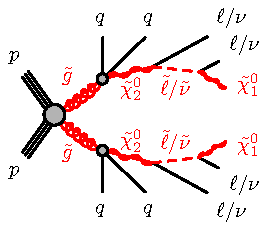
\includegraphics[width=\textwidth]{FIGURES/gogo-qqqqllllN1N1-N2}\caption{}\label{fig:feynman_gg2sl}
\end{subfigure}
\begin{subfigure}[t]{0.24\textwidth}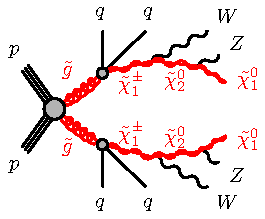
\includegraphics[width=\textwidth]{FIGURES/gogo-qqqqWWZZN1N1-C1N2}\caption{}\label{fig:feynman_gg2WZ}\end{subfigure}
\begin{subfigure}[t]{0.24\textwidth}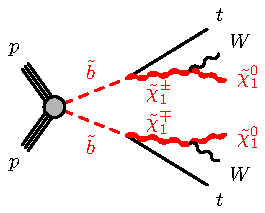
\includegraphics[width=\textwidth]{FIGURES/sbsb-ttWWN1N1}\caption{}\label{fig:feynman_b1b1}\end{subfigure}
\begin{subfigure}[t]{0.24\textwidth}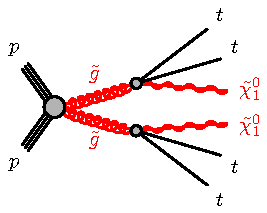
\includegraphics[width=\textwidth]{FIGURES/gogo-ttttN1N1}\caption{}\label{fig:feynman_gtt}\end{subfigure}
\caption{SUSY processes featuring gluino (a, b, d) or bottom squark (c) pair production considered in this analysis.}
\label{fig:feynman}
\end{figure}

Four signal regions (SRs) are designed to achieve good sensitivity for these SUSY scenarios, mainly characterised by the number of $b$-tagged jets or reconstructed leptons. 
They are detailed in Section~\ref{sec:selection}, preceded by descriptions of the experimental apparatus~(Section~\ref{sec:detector}) and
the simulated samples~(Section~\ref{sec:dataMC}).
Section~\ref{sec:bkg} is devoted to the estimation of the
contribution from SM processes to the signal regions, 
validated by comparisons with data in dedicated regions. 
The results are presented in Section~\ref{sec:result}, 
together with the statistical tests used to interpret the results in the context of the SUSY benchmark scenarios. 
Finally, Section~\ref{sec:conclusion} summarises the main conclusions of this paper.

%-------------------------------------------------------------------------------
\section{The ATLAS detector}
\label{sec:detector}
%-------------------------------------------------------------------------------

The ATLAS experiment~\cite{PERF-2007-01} is a multi-purpose particle detector with a forward-backward symmetric cylindrical
geometry and nearly $4\pi$ coverage in solid angle.\footnote{ATLAS uses
  a right-handed coordinate system with its origin at the nominal
  interaction point (IP) in the centre of the detector and the
  $z$-axis along the beam pipe. The $x$-axis points from the IP to the
  centre of the LHC ring, and the $y$-axis points upward. Cylindrical
  coordinates ($r$, $\phi$) are used in the transverse plane, $\phi$
  being the azimuthal angle around the beam pipe. The pseudorapidity
  is defined in terms of the polar angle $\theta$ as $\eta = -\ln
  \tan(\theta/2)$. Rapidity is defined as $y=0.5 \ln\left[(E + p_z )/(E - p_z )\right]$ where $E$ denotes the energy and $p_z$ is the component of the momentum along the beam direction.}
The interaction point is surrounded by an inner detector (ID), a
calorimeter system, and a muon spectrometer.

The ID provides precision tracking of charged particles for
pseudorapidities $|\eta| < 2.5$ and is surrounded by a superconducting solenoid providing a \SI{2}{T} axial magnetic field.
It consists of pixel and silicon-microstrip detectors inside a
transition radiation tracker.  
One significant upgrade for the $\sqrt{s}=13$~TeV running period is the presence of the
Insertable B-Layer~\cite{CERN-LHCC-2010-013}, an additional pixel layer close to the interaction point, which 
provides high-resolution hits at small radius to improve the tracking performance.

In the pseudorapidity region $|\eta| < 3.2$, high-granularity lead/liquid-argon (LAr)
electromagnetic (EM) sampling calorimeters are used.
A steel/scintillator tile calorimeter measures hadron energies for
$|\eta| < 1.7$.
The endcap and forward regions, spanning $1.5<|\eta| <4.9$, are 
instrumented with LAr calorimeters for both the EM and hadronic
measurements.

The muon spectrometer consists of three large superconducting toroids
with eight coils each, 
a system of trigger and precision-tracking chambers, 
which provide triggering and tracking capabilities in the
ranges $|\eta| < 2.4$ and $|\eta| < 2.7$, respectively.

A two-level trigger system is used to select events. The first-level
trigger is implemented in hardware and uses a subset of the detector
information. This is followed by the software-based High-Level Trigger stage,
which can run offline reconstruction and
calibration software, reducing the event rate to about \SI{1}{kHz}.



%-------------------------------------------------------------------------------
\section{Dataset and simulated event samples}
\label{sec:dataMC}
%-------------------------------------------------------------------------------

The data were collected by the ATLAS detector during 2015 and 2016 with a peak 
instantaneous luminosity of $L~=~1.4\times~10^{34}$~cm$^{-2}$s$^{-1}$. 
The mean number of $pp$ interactions per bunch crossing 
(pile-up) in the dataset is $\langle \mu \rangle = 23.7$ and
the bunch spacing is 25ns. After the application of beam, detector and data quality requirements, 
the integrated luminosity considered in this analysis corresponds to 36.0~fb$^{-1}$.
The preliminary uncertainty on the combined 2015+2016 integrated luminosity is 3.2\%. 
It is derived, following a methodology similar to that detailed in Ref.~\cite{Aaboud:2016hhf}, 
from a preliminary calibration of the luminosity scale using $x$-$y$ beam-separation scans performed in August 2015 and May 2016.

Monte Carlo (MC) simulated event samples are used to estimate the irreducible SM background with two 
same-sign and or three prompt leptons to model the SUSY signals. The reducible background, mainly 
coming from $\ttbar$ production, is estimated from the data as described in detail in Section~\ref{sec:bkg}. 
The MC samples are processed through an ATLAS detector simulation~\cite{Aad:2010ah} based on 
{\sc Geant4}~\cite{Agostinelli:2002hh} or a fast simulation using a parameterisation of the calorimeter response 
and {\sc Geant4} for the ID and MS~\cite{ATL-PHYS-PUB-2010-013}. To simulate the effects of additional $pp$ collisions 
in the same and nearby bunch crossings, additional interactions are generated using the soft QCD processes 
of \PYTHIA 8.186~\cite{Sjostrand:2007gs} with the A2 tune~\cite{ATLAS-PHYS-PUB-2012-003} and the MSTW2008LO PDF~\cite{Martin:2009iq}, 
and overlaid onto the simulated hard scatter event. 
The MC events are reweighted to match the pile-up conditions observed in the data and are reconstructed in the 
same manner as the data. The generator, parton shower, cross-section normalisation, parton distribution function (PDF) 
set and underlying-event tune of all samples are given in Table~\ref{tab:MC}.In all MC samples, except 
those produced by \SHERPA, the {\sc EvtGen}~v1.2.0 program~\cite{EvtGen} is used to model the properties 
of the bottom and charm hadron decays. 



\begin{table*}[ht]
\begin{center}
\scriptsize
\resizebox{\textwidth}{!}
{
\begin{tabular}{|l|l|c|c|c|c|}
\hline
Physics process    & Generator & Parton shower & Cross-section & PDF set & Tune \\
                   &	      & 	      & normalisation & 	&      \\
\hline
RPC signal 	   & \AMCATNLO 2.2.3~\cite{Alwall:2014hca} & \PYTHIA 8.186~\cite{Sjostrand:2007gs}&NLO+NLL~\cite{Beenakker:1996ch,Kulesza:2008jb,Kulesza:2009kq,Beenakker:2009ha,Beenakker:2011fu,Kramer:2012bx} & NNPDF2.3LO~\cite{Lai:2010vv} & A14~\cite{pub-2014-021} \\
        	   &  		           & 		       & or NLO-Prospino2 			& 			     &   \\
RPV signal 	   & \AMCATNLO 2.2.3        & \PYTHIA 8.210       & NLO+NLL or			 & NNPDF2.3LO		       & A14 \\
        	   &  		           & 		       & NLO-Prospino2 			& 			     &   \\
\hline
$\ttbar+W/Z/\gamma^{*}$ & \AMCATNLO 2.2.2 & \PYTHIA 8.186	  & NLO~\cite{YR4}     & NNPDF2.3LO & A14    \\
$\ttbar H$	   & \AMCATNLO 2.2.2        & \HERWIG 2.7.1~\cite{Corcella:2000bw}                & NLO~\cite{YR4}   &
CTEQ6L1~\cite{Pumplin:2002vw} & UEEE5~\cite{Gieseke:2012ft}  \\
$\ttbar\ttbar$     & \AMCATNLO 2.2.2       & \PYTHIA 8.186        & NLO~\cite{Alwall:2014hca}	  & NNPDF2.3LO	  & A14  \\
Diboson    & \SHERPA 2.1.1~\cite{gleisberg:2008ta}               & \SHERPA 2.1.1	& NLO~\cite{pubnote_mc_multiboson}	 &CT10~\cite{Lai:2010vv} & \SHERPA default \\
\hline
$\ttbar+WW/WZ$     & \AMCATNLO 2.2.2       & \PYTHIA 8.186         & NLO~\cite{Alwall:2014hca}	  & NNPDF2.3LO	  & A14  \\
$t+Z/WZ/\ttbar$    & \AMCATNLO 2.2.2        & \PYTHIA 8.186       & LO~\cite{YR4}                   	 & NNPDF2.3LO     & A14  \\
Triboson	   & \SHERPA 2.1.1         & \SHERPA 2.1.1        & LO, NLO~\cite{pubnote_mc_multiboson}            & CT10	     & \SHERPA default \\
$H+W/Z$	           & \AMCATNLO 2.2.2        & \PYTHIA 8.186       & NLO~\cite{Dittmaier:2012vm}   & NNPDF2.3LO     & A14  \\
\hline
\end{tabular}
}
\caption{Simulated signal and background event samples: the corresponding generator, parton shower, cross-section normalisation, PDF set and 
underlying-event tune are shown. Because of their very small contribution to the signal region background estimate 
$\ttbar+WW/WZ$, $t+Z/WZ/\ttbar$, $H+W/Z$ and triboson are summed and called ``Rare'' in the following. 
NLO-Prospino2 refers to RPV down squark models of Fig.\ref{fig:feynm_rpv_sd313} and \ref{fig:feynm_rpv_sd321}, as well as NUHM2.}
\label{tab:MC}
\end{center}
\end{table*}

The SUSY signals are defined by an effective Lagrangian describing the interactions of a small number of new 
particles~\cite{Alwall:2008ve,Alwall:2008ag,Alves:2011wf}. All SUSY particles not included 
in the decay of the pair-produced squarks and gluinos have their masses effectively decoupled. These models assume one 
production process and one decay channel with a 100\% branching fraction. They are generated 
from Leading Order (LO) matrix elements with up to two extra partons in the matrix element 
(only up to one for the $\gluino\to q\bar q(\ell\ell/\nu\nu)\neut$ model) 
using \AMCATNLO 2.2.3~\cite{Alwall:2014hca} interfaced to Pythia 8.186 with the A14 tune~\cite{pub-2014-021} for the 
modelling of the parton shower, hadronisation and underlying event.
Jet--parton matching is realised following the CKKW-L prescription~\cite{Lonnblad:2011xx}, with a matching scale set to one quarter of 
the pair-produced superpartner mass. The PDF set used for the generation is NNPDF23LO~\cite{Lai:2010vv}. All signal models are generated 
with prompt decays of the SUSY particles. Signal cross-sections are calculated to NLO in the strong coupling constant, 
adding the resummation of soft gluon emission at next-to-leading-logarithmic 
accuracy (NLO+NLL)~\cite{Beenakker:1996ch,Kulesza:2008jb,Kulesza:2009kq,Beenakker:2009ha,Beenakker:2011fu}, except 
for the RPV models of Fig.\ref{fig:feynm_rpv_sd313} and Fig.\ref{fig:feynm_rpv_sd321} as well as the NUHM2 model where NLO 
cross-sections are used~\cite{Beenakker:1996ed,Beenakker:1996ch}. The nominal cross-sections and the uncertainties are taken from 
envelopes of cross-section predictions using different PDF sets 
and factorisation and renormalisation scales, as described in Ref.~\cite{Kramer:2012bx}. 
Typical production cross-sections are: $(4.7 \pm 1.2)$~fb for gluino pairs with a mass of \SI{1.7}{\TeV}, $(28.3 \pm 4.0)$~fb
for bottom squark pairs with a mass of \SI{800}{\GeV}, and $(15.0\pm 2.0)$~fb for right-handed down 
squark pairs with a mass of \SI{800}{\GeV} and a gluino mass of \SI{2.0}{\TeV}.

The two dominant background processes are $\ttbar V$ (with $V=W$ and $Z$, including non-resonant $Z/\gamma^*$ contributions) 
and diboson with four charged leptons ($\ell$ including here all lepton flavors, where $\tau$
leptons subsequently can decay leptonically or hadronically), three charged leptons and one neutrino, or 
two same-sign charged leptons and two neutrinos. They are described in details in Refs.~\cite{pubnote_mc_ttv} and~\cite{pubnote_mc_multiboson}, 
respectively. Samples of the former are generated with one ($\ttbar Z$) and two ($\ttbar W$) extra partons. Similarly for the latter, 
one ($W^\pm W^\pm jj$) and two ($WZ$, $ZZ$) extra partons are simulated. NLO cross-sections for 
$\ttbar W$, $\ttbar Z/\gamma^*(\rightarrow \ell \ell)$ and dibosons are respectively 600.8~fb~\cite{YR4}, 
123.7~fb\footnote{This cross-section is computed using the configuration of Refs.~\cite{Alwall:2014hca,Frixione:2015zaa}.} and 
40.0~pb~\cite{pubnote_mc_multiboson}. The processes $\ttbar H$ and $\ttbar \ttbar$, with NLO cross-sections of 507.1~fb~\cite{YR4} and 
9.2~fb~\cite{Alwall:2014hca} respectively, are also considered.

Other low cross-section background processes are grouped into ``Rare'' in the following. This category contains 
samples of $\ttbar+WW/WZ$ with no extra parton in the matrix element, $t+Z/WZ/\ttbar$, $H+W/Z$ as well as 
triboson ($WWW$, $WWZ$, $WZZ$ and $ZZZ$) production with up to six charged leptons. The $4\ell$ and $2\ell+2\nu$ processes are 
calculated at NLO with up to one additional parton; final states with two and three additional partons are calculated at leading order (LO). 
The $WWZ\to 4\ell+2\nu$ or $2\ell+4\nu$ processes are calculated at LO with up to two additional partons. 
The $3\ell +1\nu$ process is calculated at NLO with up to three extra partons at LO using the Comix~\cite{Gleisberg:2008fv} 
and OpenLoops~\cite{Cascioli:2011va} matrix element generators and merged with the \SHERPA~\cite{Schumann:2007mg} 
using the ME+PS@NLO prescription for the parton shower~\cite{Hoeche:2012yf}. The $WWZ/WZZ\to 3\ell+3\nu$, $ZZZ\to 6\ell+0\nu$, $4\ell+2\nu$ or $2\ell+4\nu$ processes 
are calculated with the same configuration but with up to only two extra partons at LO.


%-------------------------------------------------------------------------------
\section{Event selection}
\label{sec:selection}
%-------------------------------------------------------------------------------

Candidate events are required to have a reconstructed vertex~\cite{ATL-PHYS-PUB-2015-026}, 
with at least two associated tracks with $\pt >400$~MeV, 
and the vertex with the highest sum of squared transverse 
momentum of the tracks is considered as primary vertex.
In order to perform background estimations using data, 
two categories of electrons and muons are defined: 
``candidate'' and ``signal'' (the latter being a subset of the ``candidate'' leptons satisfying tighter selection criteria). 

Electron candidates are reconstructed from an isolated electromagnetic 
calorimeter energy deposit matched to an ID track and are required to have $|\eta|<2.47$, 
a transverse momentum $\pT>\SI{10}{\GeV}$, 
and to pass a loose likelihood-based identification requirement~\cite{elecperf,ATL-PHYS-PUB-2015-041}. 
The likelihood input variables include measurements of calorimeter shower shapes and measurements of track properties from the ID. 
Candidates within the transition region between the barrel and endcap electromagnetic calorimeters,
$1.37<|\eta|<1.52$, are removed. 
The track matched with the electron must have a significance of the transverse impact parameter 
with respect to the reconstructed primary vertex, $d_0$, of $\vert d_0\vert/\sigma(d_0) < 5$.

Muon candidates are reconstructed in the region $|\eta|<2.5$ 
from muon spectrometer tracks matching ID tracks.
All muons must have $\pT>\SI{10}{\GeV}$ and must pass the medium identification requirements defined in Ref.~\cite{Run2Muon}, 
based on selections on the number of hits in the different ID and muon spectrometer subsystems, 
and the significance of the charge to momentum ratio $q/p$~\cite{Run2Muon}.

Jets are reconstructed with the anti-$k_t$
algorithm~\cite{Cacciari:2008} with radius parameter $R=0.4$, using three-dimensional energy
clusters in the calorimeter~\cite{caloclusters} as input. 
All jets must have $\pT>\SI{20}{\GeV}$ and $|\eta|<2.8$.
Jets are calibrated as described in Ref.~\cite{ATLAS-PHYS-PUB-2015-015}.
In order to reduce the effects of pile-up, 
for jets with $\pt<\SI{50}{GeV}$ and $|\eta|<2.4$ a significant fraction of the tracks associated with each jet
must have an origin compatible with the primary vertex, 
as defined by the jet vertex tagger~\cite{ATLAS-CONF-2014-018}. 
Furthermore, for all jets the expected average energy contribution from
pile-up clusters is subtracted according to the jet area~\cite{ATLAS-PHYS-PUB-2015-015}.

Identification of jets containing $b$-hadrons ($b$-tagging) is performed with the MV2c20 algorithm, 
a multivariate discriminant making use of track impact parameters 
and reconstructed secondary vertices~\cite{Aad:2015ydr,ATL-PHYS-PUB-2015-022}.
A requirement is chosen corresponding to a 70\% average efficiency 
obtained for $b$-jets in simulated $\ttbar$ events. 
The rejection factors for light-quark jets, $c$-quark jets and hadronically decaying $\tau$ leptons in simulated $\ttbar$ events 
are approximately 440, 8 and 26, respectively~\cite{ATL-PHYS-PUB-2015-022}. 
Jets with $|\eta|<2.5$ which satisfy this $b$-tagging requirement are identified as $b$-jets. 
To compensate for differences between data and MC simulation in the $b$-tagging efficiencies and mis-tag rates, 
correction factors are applied to the simulated samples~\cite{ATL-PHYS-PUB-2015-022}. 

After object identification, overlaps between objects are resolved. 
Any jet within a distance $\Delta R_y =\sqrt{(\Delta y)^2+(\Delta\phi)^2}$ = 0.2 of an electron candidate is discarded, 
unless the jet has a value of the MV2c20 discriminant larger than the value corresponding to approximately an 80\% $b$-tagging efficiency, 
in which case the electron is discarded since it is likely originating from a semileptonic $b$-hadron decay. 
Any remaining electron within $\Delta R_y=$ 0.4 of a jet is discarded. 
Muons within $\Delta R_y=$ 0.4 of a jet are also removed. 
However, if the jet has fewer than three associated tracks, the muon is kept and the jet is discarded instead 
to avoid inefficiencies for high-energy muons undergoing significant energy loss in the calorimeter.

Signal electrons must satisfy a tight likelihood-based identification requirement~\cite{elecperf,ATL-PHYS-PUB-2015-041} 
and have $|\eta|<2$ to reduce the impact of electron charge mis-identification. 
Signal muons must fulfil the requirement of $\vert d_0\vert/\sigma(d_0) < 3$. 
The track associated to the signal leptons must have a longitudinal impact parameter with respect to the reconstructed primary vertex, $z_0$, 
satisfying $\vert z_0 \sin\theta\vert  < 0.5$~mm. 
Isolation requirements are applied to both the signal electrons and muons. 
The  scalar sum of the \pt of tracks within a variable-size cone around the lepton, 
excluding its own track, must be less than 6\% of the lepton \pt. 
The track isolation cone radius for electrons (muons) 
$\Delta R_\eta=\sqrt{(\Delta\eta)^2+(\Delta\phi)^2}$ 
is given by 
the smaller of $\Delta R_\eta = \SI{10}{~GeV}/\pt$ and $\Delta R_\eta = 0.2\,(0.3)$, 
that is, a cone of size $0.2\,(0.3)$ at low $\pt$ but narrower for high-\pt leptons. 
In addition, in the case of electrons the energy of calorimeter energy clusters in a cone of $\Delta R_\eta = 0.2$ around the electron 
(excluding the deposition from the electron itself) must be less than 6\% of the electron \pt. 
Simulated events are corrected to account for minor differences in the lepton trigger, reconstruction and 
identification efficiencies between data and MC simulation.

The missing transverse momentum ${\vec p}^{\rm miss}_{\rm T}$ is defined as the negative vector sum of the transverse momenta of all identified physics objects (electrons, photons, muons, jets) and an additional soft term. The soft term is constructed from all tracks that are not associated with any physics object, and that are associated with the primary vertex. In this way, the $\met$ is adjusted for the best calibration of the jets and the other identified physics objects above, while maintaining pile-up independence in the soft term~\cite{ATL-PHYS-PUB-2015-027, ATL-PHYS-PUB-2015-023}.

Events are selected using a combination (logical OR) of dilepton and $\met$ triggers, 
the latter being used only for events with $\met>\SI{250}{GeV}$. 
The trigger-level requirements on $\met$ and the leading and subleading lepton \pt are looser than those applied offline 
to ensure that trigger efficiencies are constant in the relevant phase space. 
Events of interest are selected if they contain at least two signal leptons with $\pt>20$~\GeV . 
If the event contains exactly two signal leptons, they are required to have the same electric charge. 

To maximise the sensitivity in different signal models, 
four overlapping signal regions are defined as shown in Table~\ref{tab:SRdef3}, with requirements on the number of signal leptons ($N_{\rm{lept}}^{\rm{signal}}$), 
the number of $b$-jets with $\pt>\SI{20}{\GeV}$ ($N_{b\rm{-jets}}^{20}$), 
the number of jets with $\pt>\SI{50}{\GeV}$ regardless of their flavour ($N_{\rm{jets}}^{50}$), 
\met\ 
and the effective mass (\meff), defined as the scalar sum of the $\pt$ of the signal leptons and jets (regardless of their flavour) in the event plus the \met. 

\begin{table}[tbh!]
\caption{Summary of the event selection criteria for the signal regions (see text for details).}
\hspace{0.5cm}
\def\arraystretch{1.3}
\label{tab:SRdef3}
\centering
\begin{tabular}{c|c|c|c|c|c}
\hline 
\hline
Signal region  &  $N_{\rm{lept}}^{\rm{signal}}$   & $N_{b\rm{-jets}}^{20}$    & $N_{\rm{jets}}^{50}$  & \met\ [GeV] & \meff\ [GeV]   \\
\hline\hline
SR0b3j &  $\ge$3  &    $=$0 &  $\ge$3 &  $>$200 & $>$550 \\
SR0b5j &  $\ge$2  &    $=$0 &  $\ge$5 &  $>$125 & $>$650 \\
SR1b     &  $\ge$2  &    $\ge$1  &  $\ge$4 &  $>$150 & $>$550 \\
SR3b     &   $\ge$2  &   $\ge$3  &  - & $>$125 & $>$650   \\
\hline\hline
\end{tabular}
\end{table}

Each signal region is motivated by a different SUSY scenario. 
The SR0b3j and SR0b5j signal regions are sensitive to gluino-mediated and directly produced squarks of the first and second generations 
leading to final states particularly rich in leptons (Fig.~\ref{fig:feynman_gg2sl}) or in jets (Fig.~\ref{fig:feynman_gg2WZ}), 
but with no enhancement of the production of $b$-quarks. 
Third-generation squark models resulting in final states with two $b$-quarks, 
such as direct bottom squark production (Fig.~\ref{fig:feynman_b1b1}), are targeted by the SR1b signal region. 
Finally, the signal region SR3b targets gluino-mediated top squark production resulting in final states with four $b$-quarks (Fig.~\ref{fig:feynman_gtt}).

The values of acceptance times efficiency of the SR selections for the SUSY signal models 
in Fig.~\ref{fig:feynman} typically range between 1\% and 6\% for $m_{\gluino}=\SI{1.2}{TeV}$ or $m_{\sbottomone}=\SI{600}{GeV}$, and a light \ninoone.


%-------------------------------------------------------------------------------
\section{Background estimation}
\label{sec:bkg}
%-------------------------------------------------------------------------------

Two main sources of SM background can be distinguished in this analysis. 
The first category is the reducible or detector background which includes 
events containing electrons with mis-measured charge, mainly from the production of top quark pairs, and events 
containing at least one non-prompt or fake lepton (FNP), which mainly originate from hadron decays in events containing 
top quarks, $W$ or $Z$ bosons. Data-driven methods used for the estimation
of this background are described in Section~\ref{sec:DD_bkg}. The second category consists of events 
with two same-sign prompt leptons or at least three prompt leptons and is 
estimated using the MC samples described in Section~\ref{sec:dataMC}. 
Since diboson and $\ttbar V$ events are the main backgrounds in the signal regions, 
dedicated validation regions (VR) with an enhanced contribution from these processes 
are defined to verify the background predictions from the simulation (see Section~\ref{sec:valid}).


\subsection{Detector background estimation methods} 
\label{sec:DD_bkg}

Background events due to charge mis-identification concerns only the electron. The probability of mis-identifying the 
charge of a muon is checked in both data and MC simulation, and found to be negligible in the kinematic range relevant to this analysis.
The contribution of charge-flip events to the SR/VR yields is estimated using the data. 
The electron charge-flip probability is extracted in a $Z/\gamma^{*}\to ee$ data sample using a likelihood fit 
which takes as input the numbers of same-sign and opposite-sign electron pairs observed in a window around the $Z$ mass. 
The charge-flip probability is a free parameter of the fit and is extracted as a function of the electron $\pt$ and $\eta$. 
These probabilities are in the range \textcolor{red}{UPDATE:1--5\%} and \textcolor{red}{UPDATE:0.1--1\%} for the candidate 
and signal electrons respectively.
The event yield of this background in the signal or validation regions is obtained by applying the measured charge-flip probability 
to the data regions with the same kinematic requirements as the signal or validation regions but with opposite-sign lepton pairs. 

The contribution from fake or non-prompt leptons (such as hadrons mis-identified as leptons, 
leptons originating from heavy-flavour decays, and electrons from photon conversions) 
is also estimated from the data with a matrix method similar to that described in Ref.~\cite{SUSY3bjetsRun1}. 
In this method, two types of lepton identification criteria are defined: ``tight'', 
corresponding to the signal lepton criteria described in Section~\ref{sec:selection}, 
and ``loose'', corresponding to candidate leptons after overlap removal. 
The matrix method relates the number of events containing prompt or FNP leptons 
to the number of observed events with tight or loose-not-tight leptons 
using the probability for loose prompt or FNP leptons to satisfy the tight criteria. 
The probability for loose prompt leptons to satisfy the tight selection criteria ($\epsilon$)
is obtained using a $Z/\gamma^*\to\ell\ell$ data sample 
and is modelled as a function of the lepton $\pt$ and $\eta$. 
The probability for loose FNP leptons to satisfy the tight selection criteria (FNP fake rate, $f$) is determined from data 
in SS and three lepton control regions enriched in non-prompt leptons originating from heavy-flavour decays, mostly coming from 
semileptonic $\ttbar$ events. This region contains events with at least one $b$-jet, 
one well-isolated ``tag'' muon, and an additional loose electron or muon on which the measurement is performed. 
The efficiencies are measured as function of \pt ($\eta$ binning is also used for low \pt muons) 
after subtracting the small contribution from prompt lepton processes. 

\textcolor{red}{[UPDATE: rewrite/inflate this paragraph]}The estimated FNP yields in the SRs are consistent with those 
predicted by two alternative methods: the first one relies on MC simulation of processes with FNP leptons or charge-flipped electrons 
($\ttbar$, $V$+jets)~\cite{paperSS3L,ATLAS-CONF-2012-151}, 
corrected to match the observed data in dedicated control regions. 
The second method relies on data events with only one lepton, which are the processes leading to FNP leptons, 
to extrapolate from low-\met\ control regions to the SRs.

%The data-driven background estimates are cross-checked with an MC-based technique. 
%In this method, the contributions from processes with FNP leptons and electron charge mis-identification 
%are obtained from MC simulation and normalised to data in dedicated control regions at low jet multiplicity, low $\met$, and 
%either with or without $b$-jets. 
%The normalisation is performed using five multipliers: one to correct 
%the electron charge mis-identification rate, and four to correct the contributions from FNP 
%electrons or muons originating from $b$-jets or light-flavour jets, respectively.
%In addition to the MC samples listed in Section~\ref{sec:dataMC}, this method employs samples of top quark pair production generated with the \POWHEG-Box v2 generator interfaced to \PYTHIA 6.428~\cite{Sjostrand:2006za}, 
%as well as samples of simulated $W$+jets and $Z$+jets events generated with \POWHEG-Box v2 interfaced to \PYTHIA 8.186.

% not the best place, but otherwise it's not well positionned wrt the text...
\begin{figure}[th!]
\centering
\begin{subfigure}[t]{0.49\textwidth}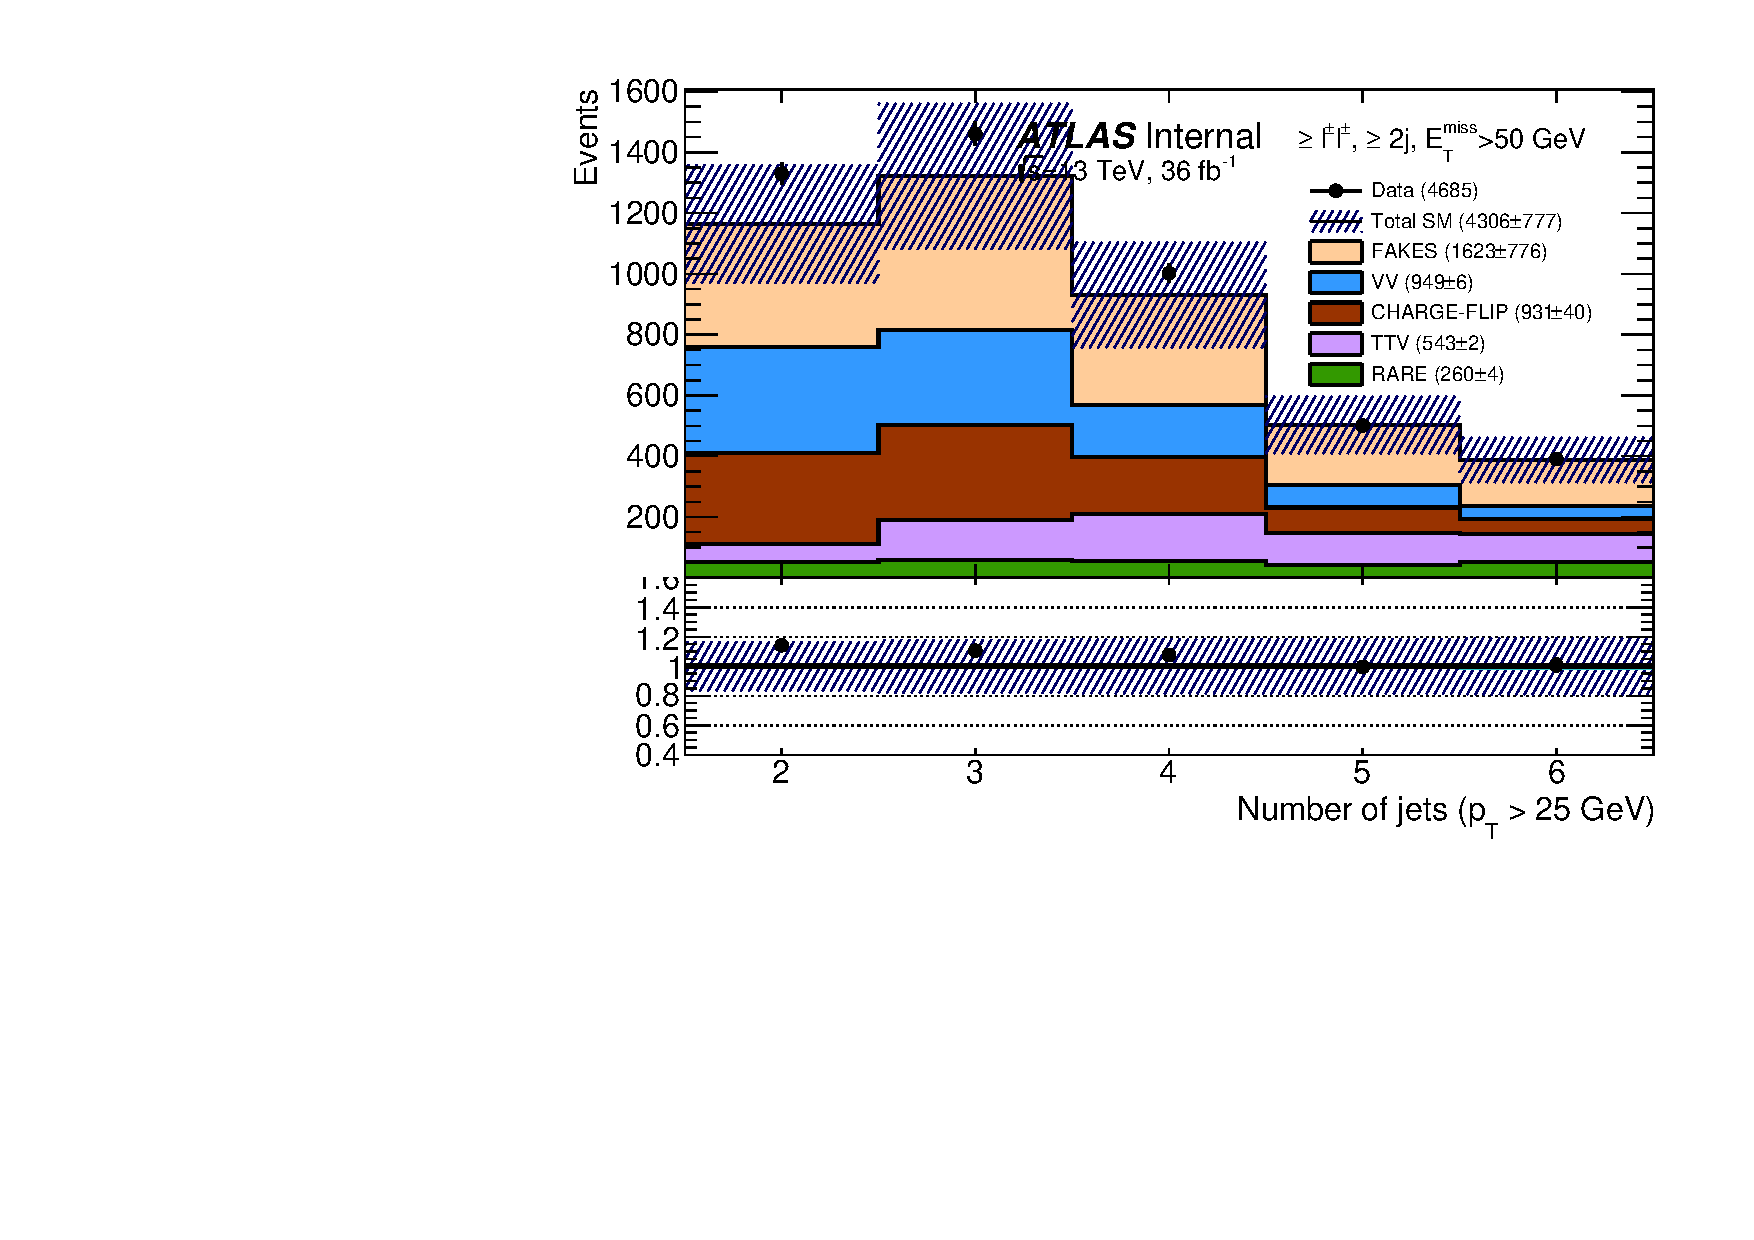
\includegraphics[width=\textwidth]{DILEP_2JMET50_njets25}\caption{}\end{subfigure}
\begin{subfigure}[t]{0.49\textwidth}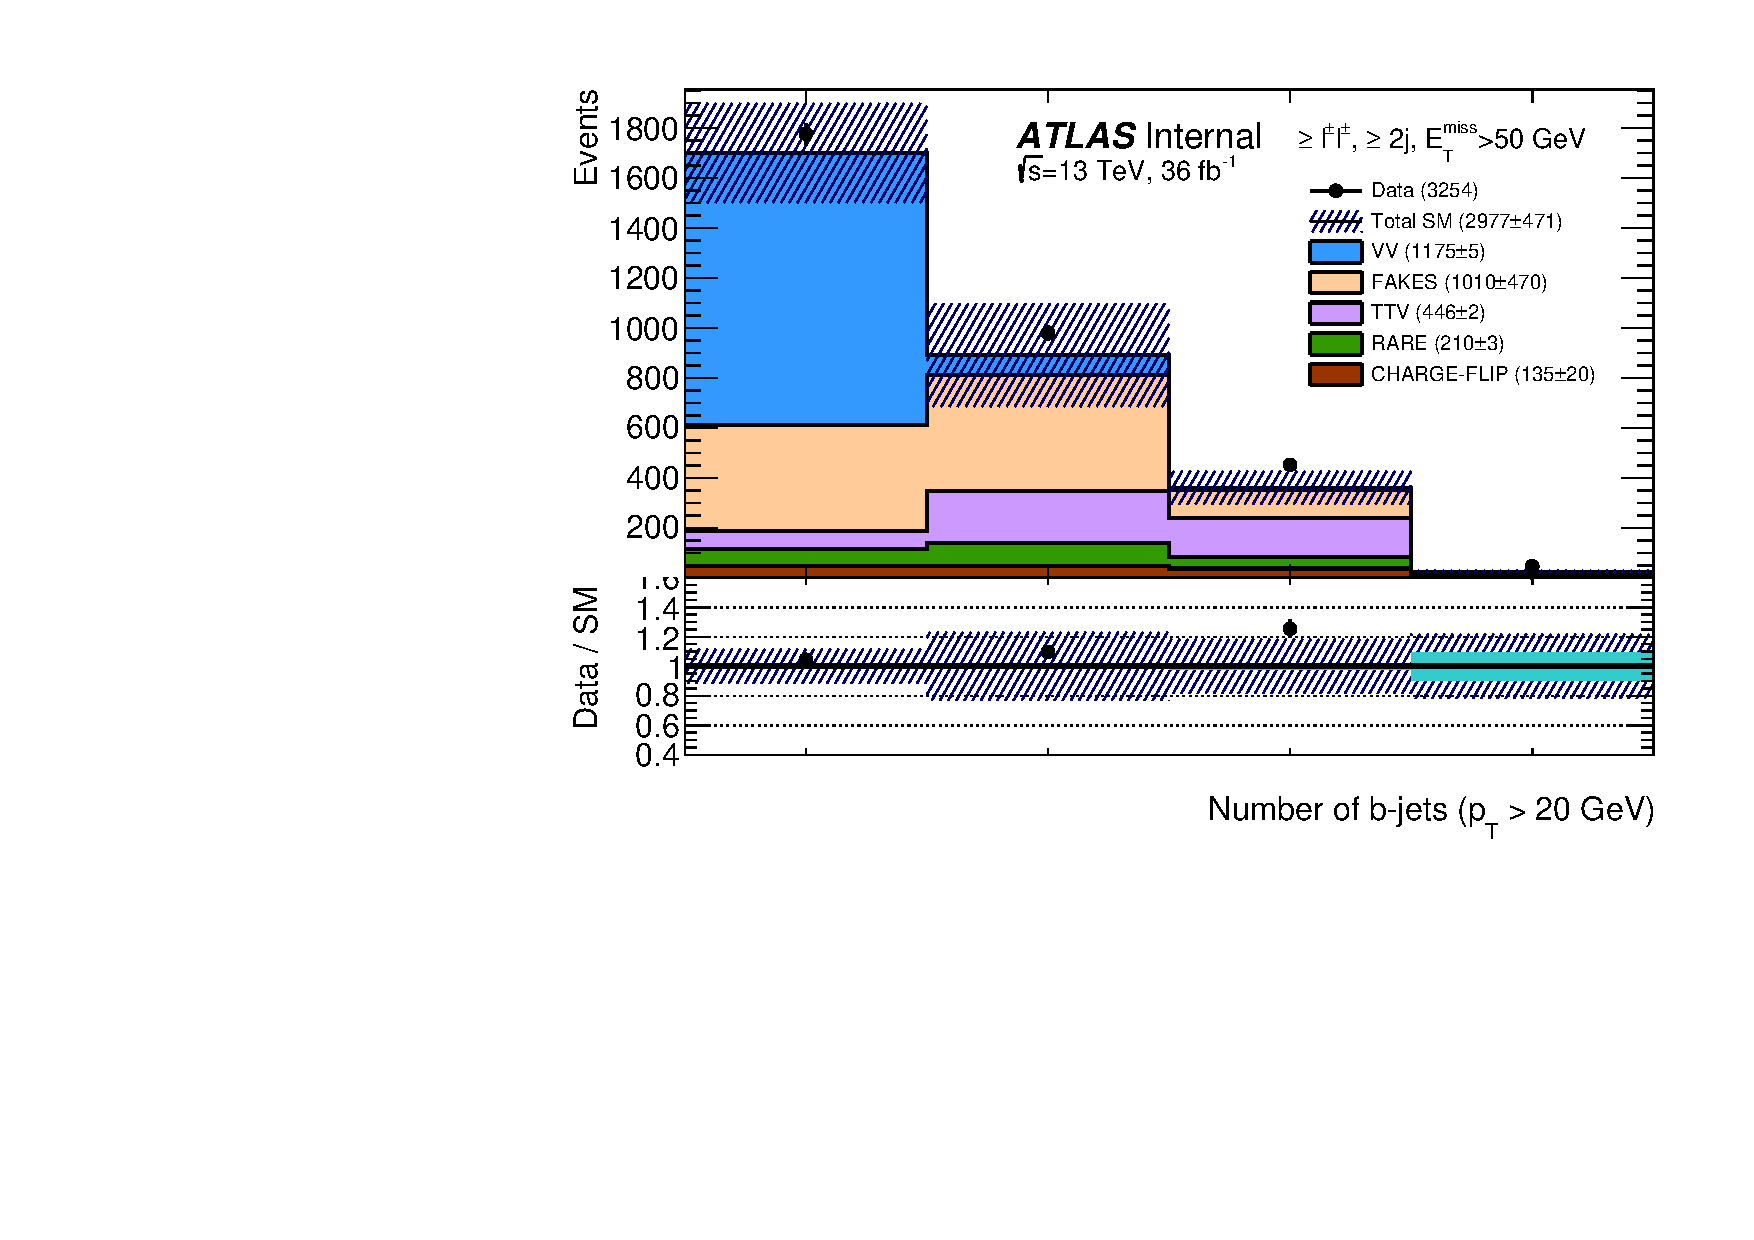
\includegraphics[width=\textwidth]{DILEP_2JMET50_nbjets}\caption{}\end{subfigure}
\begin{subfigure}[t]{0.49\textwidth}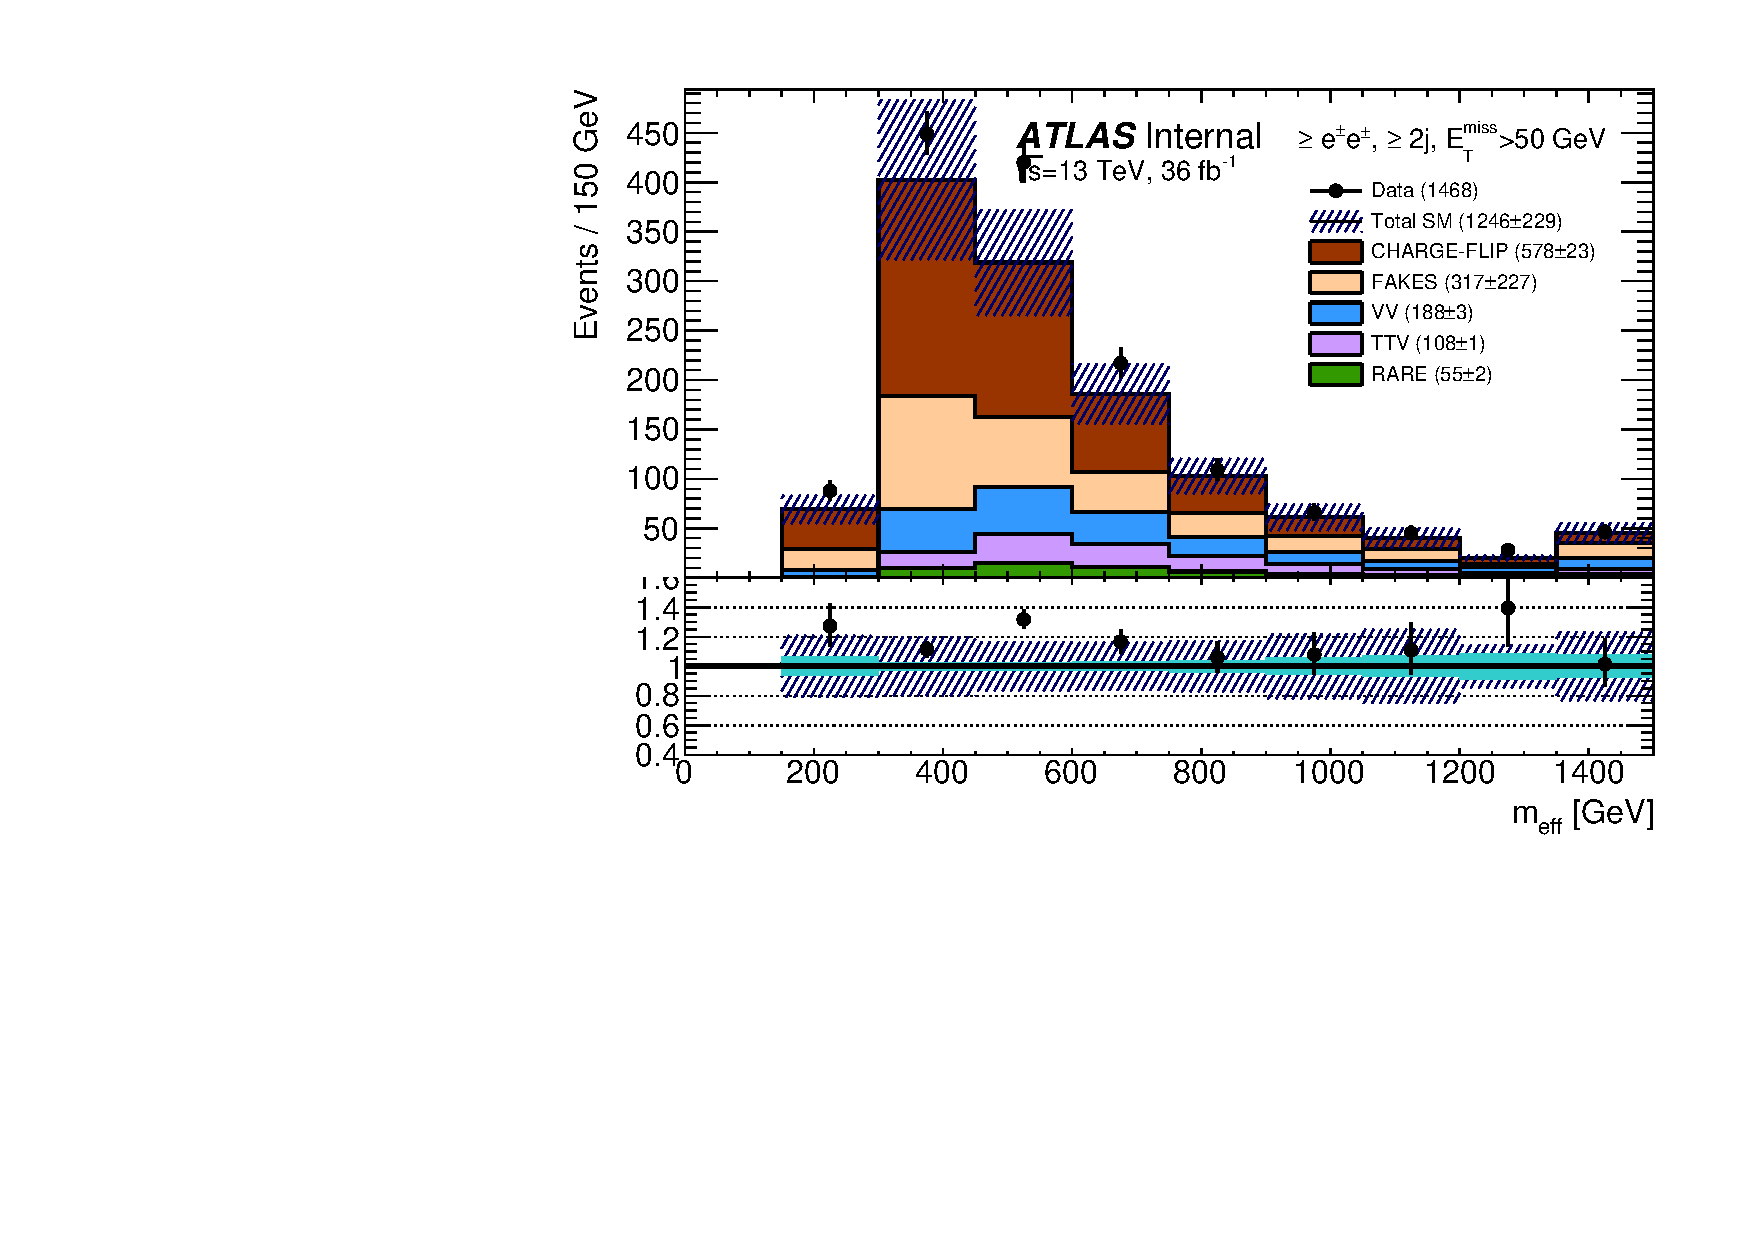
\includegraphics[width=\textwidth]{EE_2JMET50_meff}\caption{}\end{subfigure}
\begin{subfigure}[t]{0.49\textwidth}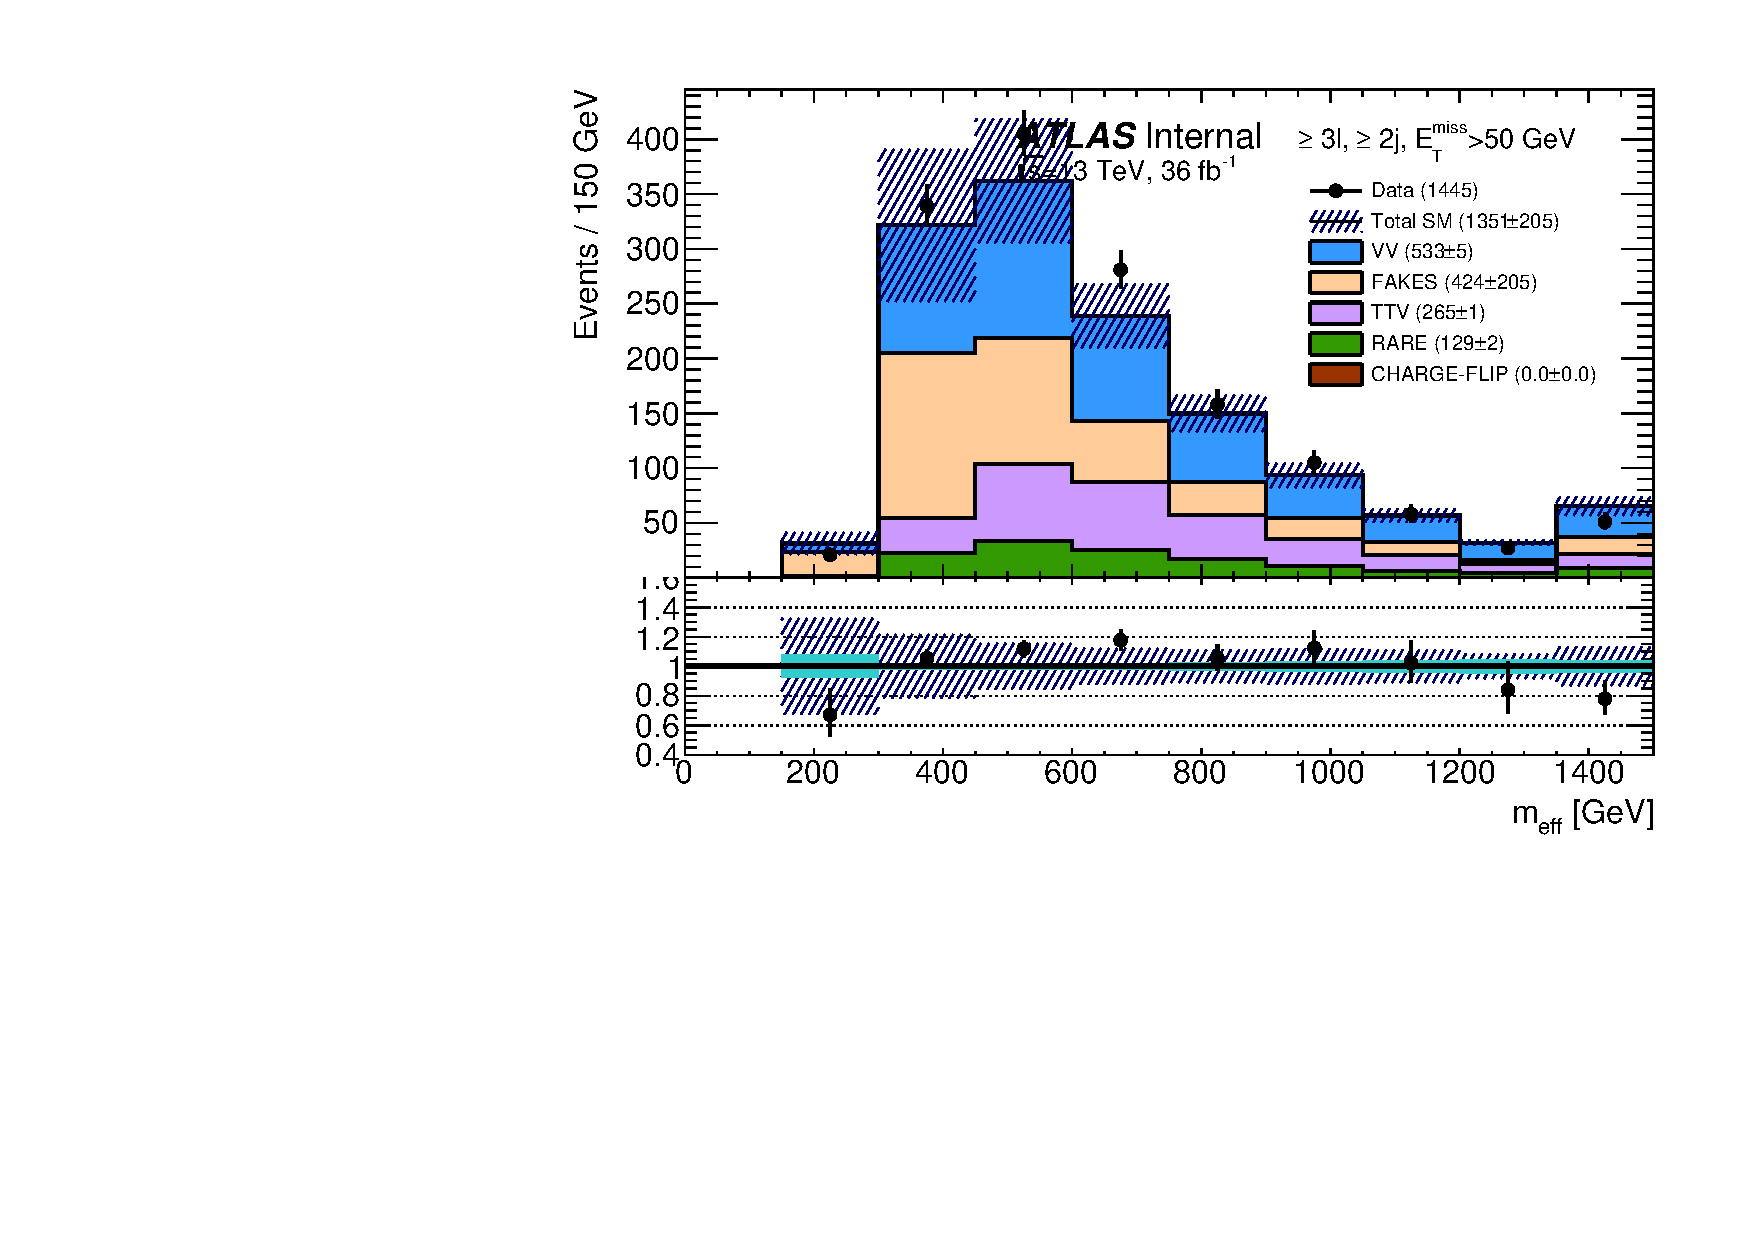
\includegraphics[width=\textwidth]{TRILEP_2JMET50_meff}\caption{}\end{subfigure}
\caption{
Distributions of the number of jets, of $b$-tagged jets and the effective mass after requiring at least two jets ($\pT>\SI{25}{GeV}$) and $\met>\SI{50}{GeV}$, 
as well as at least two same-sign leptons (a,b) or two same-sign electrons (c) or three leptons (d). 
The statistical uncertainties in the background prediction are included in the uncertainty band, 
as well as the full systematic uncertainties for backgrounds with fake or non-prompt leptons, or charge-flip. 
The light blue bands in the ratio plots show contributions from statistical uncertainties alone while the hashed area shows the total uncertainty.. 
The ``Rare'' category contains the contributions from associated production $\ttbar+WW/WZ$, 
as well as $t+Z/WZ/\ttbar$, $H+W/Z$, and triboson production. \textcolor{red}{[UPDATE: Remove numbers in the legend 
and move from upper case to lower case.]}
}
\label{fig:Bkg_distribs} 
\end{figure} 


\subsection{Validation of background estimates}
\label{sec:valid}

To check the validity and robustness of the background estimates, 
the distributions of several discriminating variables in data are compared 
with the predicted background after various requirements on the number of jets and $b$-jets. 
%Events are categorised based on the flavours of the selected leptons, and the different flavour channels are compared separately. 
Examples of such distributions are shown in Fig.~\ref{fig:Bkg_distribs}, 
and illustrate that the predictions and data agree fairly well. 

Dedicated validation regions are defined to test the estimate of the $\ttbar V$, $WZ$ and $W^\pm W^\pm$ SM processes contributing to the signal regions. The corresponding selections are summarized in Table~\ref{tab:VRdef}. 
In these regions, the overlap with the signal regions is resolved by vetoing events that contribute to the signal regions.  
%To further reduce contributions from electron charge mis-identification,  events are also vetoed in VR-$\ttbar W$ and VR-$W^\pm W^{\pm}jj$ if one of the two leading leptons is an electron with $|\eta|>1.37$\textcolor{red}{[UPDATE:Still true]}, since contributions from charge-flip electrons are smaller in the central region due to the lower amount of detector material in front of the calorimeters. 
The purity of the targeted processes in these regions ranges from about \textcolor{red}{[UPDATE:20\% to $50\%$]}. 

The observed yields in these validation regions, compared with the background predictions and uncertainties, 
can be seen in Table~\ref{tab:VR_yields}.
%, and the effective mass distributions are shown in Fig.~\ref{fig:VRd}--\ref{fig:VRf}.
There is good agreement between data and the estimated background for the validation regions.

\begin{table}[t!]
\hspace{0.5cm}
\def\arraystretch{1.1}
\centering
\resizebox{\textwidth}{!}
{\small
\begin{tabular}{|c|c|c|c|c|c|c|l|}
\hline    
Validation        &  $N_{\rm{lepton}}^{\rm{signal}}$ ($N_{\rm{lepton}}^{\rm{cand}}$)   & $N_{b\rm{-jets}}$  &  $N_{\rm{jets}}$  & $p^{}_{\rm{T,jet}}$  & \met\ & \meff\  & Other \\
Region Name       &  &  &  & [GeV]  & [GeV] & [GeV]  & \\
\hline\hline
$W^{\pm} W^{\pm}jj$ & $=2$ ($=2$)    &  $=0$ & $\geq 2$ &   $>50$ & $> 55$  & $> 650$ & veto $81<\mee<101$~GeV  \\
               	  & $=1$ SS pair  &	  &	     &         &   	&	  & $\pt^{\ell_2}>30$~GeV \\
               	  &		  &	  &	     &         &   	&	  & min$\left\{\Delta R(\ell_{1,2},j)\right\}>0.7$ \\
               	  &		  &	  &	     &         &   	&	  & min$\left\{\Delta R(\ell_1, \ell_2)\right\}>1.3$ \\
\hline
$WZ$4j            & $=3$ ($=3$)    &  $=0$ & $\geq 4$ &  $>25$   & --    & $> 450$ & $\met/\sum p_T^{\ell} < 0.7$ \\
\hline
$WZ$5j            & $=3$ ($=3$)    &  $=0$ & $\geq 5$ &  $>25$   & --    & $> 450$ & $\met/\sum p_T^{\ell} < 0.7$  \\ 
\hline
$\ttbar W$   	&$=2$ ($=2$)    &$\geq 1$   & $\geq 4$ ($e^\pm e^\pm$, $e^\pm \mu^\pm$) & $>40$ & $> 45$  & $> 550$   & $\pt(\ell_2)>40$~GeV\\
              	& $=1$ SS pair  &       &  $\geq 3$ ($\mu^\pm \mu^\pm$)   &  $>25$ &      &          & $\sum p_T^{b-jet}/\sum p_T^{jet}>0.25$ \\ 
\hline
$\ttbar Z$    	&$\geq 3$ (-) & $\geq 1$ & $\geq 3$ &  $>35$ &  --    & $> 450$  & $81<m_\text{SFOS}<101$~GeV \\
                &$\geq 1$ SFOS pair&     &          &       &         &         &  \\
\hline
All VRs & \multicolumn{7}{c|}{Veto events belonging to any SR} \\
\hline
\end{tabular}
}
\caption{Summary of the event selection in the validation regions (VRs). 
Requirements are placed on the number of signal leptons ($N_{\rm{lept}}^{\rm{signal}}$) 
and candidate leptons ($N_{\rm{lept}}^{\rm{cand}}$), the number of jets ($N_{\rm{jets}}$) 
or the number of $b$-jets with $\pt>\SI{20}{GeV}$ ($N_{b\rm{-jets}}$). The two leading-\pt 
leptons are referred to as $\ell_{1,2}$ with decreasing \pt. Additional requirements are set 
on \met, \meff, the invariant mass of the two leading electrons $m_{ee}$, the presence of SS 
leptons or a pair of same-flavour opposite-sign leptons (SFOS) and its invariant mass $m_\text{SFOS}$. 
A minimum angular separation between the leptons and the jets ($\Delta R (\ell, j)$) and between the two 
leptons ($\Delta R (\ell_{1}, \ell_2)$) is imposed in $W^\pm W^\pm$ VR. For the two $WZ$ VRs an upper cut 
on the ratio between the \met in the event and the sum of all selected leptons \pt (\met/$\sum{p_T^\ell}$) is required. 
An upper cut on the ratio between the sum of the \pt of all $b$-jets and that of all jets in the event ($\sum p_T^{b-j} / \sum{p_T^{j}}$) is 
considered only in the $\ttbar W$ VR.
}
\label{tab:VRdef}
\end{table}

\begin{table}[t!]
\hspace{0.5cm}
\def\arraystretch{1.1}
\centering
%\resizebox{\textwidth}{!}
%{\small
\begin{tabular}{|l|c|c|c|c|c|}
\hline    
 Validation Regions       & $WZ$4j & $WZ$5j  & $W^\pm W^{\pm}jj$& $\ttbar W$   & $\ttbar Z$  \\
\hline\hline
$t\bar{t}Z/\gamma^*$     & $  \pm  $ & $  \pm  $      & $  \pm  $  & $  \pm  $    & $  \pm  $  \\
$t\bar{t}W$              & $  \pm $  & $  \pm  $      & $  \pm  $  & $  \pm  $    & $  \pm  $  \\
$t\bar{t}H$              & $  \pm $  & $  \pm  $      & $  \pm  $  & $  \pm  $    & $  \pm  $  \\
$t\bar{t}t\bar{t}$       & $  \pm $  & $  \pm  $      & $  \pm  $  & $  \pm  $    & $  \pm  $  \\
$WW$                     & $  \pm $  & $  \pm  $      & $  \pm  $  & $  \pm  $    & $  \pm  $  \\
$WZ$                     & $  \pm $  & $  \pm  $      & $  \pm  $  & $  \pm  $    & $  \pm  $  \\
$ZZ$                     & $  \pm $  & $  \pm  $      & $  \pm  $  & $  \pm  $    & $  \pm  $  \\
Rare                     & $  \pm  $ & $  \pm  $      & $  \pm  $  & $  \pm  $    & $  \pm  $  \\
Fake/non-prompt leptons  & $  \pm  $ & $  \pm  $      & $  \pm  $  & $  \pm  $    & $  \pm $  \\
Charge-flip              & $-$       & $  \pm  $      & $  \pm  $  & $  \pm  $    & $-$  \\
\hline
Total SM  background   	& $-$        & $  \pm  $      & $  \pm  $  & $  \pm  $    & $-$  \\
\hline
Observed	   	& $-$        & $  \pm  $      & $  \pm  $  & $  \pm  $    & $-$  \\
\hline
\end{tabular}
%}
\caption{The numbers of observed data and expected background events in the validation regions. 
The ``Rare'' category contains the contributions from associated production $\ttbar+WW/WZ$, 
as well as $t+Z/WZ/\ttbar$, $H+W/Z$, and triboson production. Background categories shown as a ``$-$'' 
denote that they cannot contribute to a given region (e.g. charge flips in 3-lepton regions). 
The displayed yields include all sources of statistical and systematic uncertainties, 
except for the theoretical uncertainties which only affect the inclusive production cross-sections.}
\label{tab:VR_yields}
\end{table}

\section{Systematic uncertainties on the background estimation}
\label{sec:syst}

Figure~\ref{fig:PlotSR} summarises the contributions of the different sources of systematic uncertainty 
on the total SM background predictions in the signal regions.

The systematic uncertainties related to the same-sign prompt leptons background estimation 
arise from the accuracy of the theoretical and experimental modelling in the MC simulation.
The primary sources of systematic uncertainties are related to the jet energy scale calibration, 
jet energy resolution, $b$-tagging efficiency, and MC modelling and theoretical cross-section uncertainties. 
The statistical uncertainty of the simulated event samples is also taken into account.

The cross-sections used to normalise the MC samples are varied according to the uncertainty in the 
cross-section calculation, that is, 13\% for $\ttbar W$, 12\% for $\ttbar Z$ production~\cite{YR4}, 6\% for diboson
production~\cite{pubnote_mc_multiboson}, 8\% for $\ttbar H$~\cite{YR4} and 30\% for $\ttbar\ttbar$~\cite{Alwall:2014hca}. 
Additional uncertainties are assigned to some of these backgrounds to account for the theoritical modelling of the kinematic 
distributions in the MC simulation. For $\ttbar W$ and $\ttbar Z$, the predictions from the \AMCATNLO and \SHERPA generators are compared, 
and the renormalisation and factorisation scales used to generate these samples are varied, 
leading to a $\sim$\textcolor{red}{[UPDATE:30\%]} uncertainty on the expected SR yields for these processes. 
For dibosons, uncertainties are estimated by varying the renormalisation, factorisation and resummation scales, 
leading to a $\sim$\textcolor{red}{[UPDATE:40-50\%]} uncertainty for these processes after the SR selections. 
For $\ttbar H$, $\ttbar \ttbar$ and Rare production processes, a conservative 50\% uncertainty 
on their total contribution is assigned. 

Uncertainties in the FNP lepton background estimate are assigned due to the limited number 
of data events in the loose and tight lepton control regions.
In addition, systematic uncertainties of \textcolor{red}{[UPDATE:50-60\%]} are assigned to the FNP fake rate to account 
for potentially different 
compositions (heavy flavour, light flavour or conversions) between the regions used to measure these probabilities and the SRs, 
as well as the contamination from prompt leptons in the former regions. Similarly a \textcolor{red}{[UPDATE:5\%]} systematic is assigned to 
$\epsilon$ determination. This leads to overall FNP background uncertainties in the total background estimates 
of \textcolor{red}{[UPDATE:5--32\%]} depending on the signal region.

The uncertainty on the electron charge-flip probability mainly originates from the limited number of events used in 
the charge-flip probability measurement regions and the uncertainty related to the background subtraction 
beyond the $Z$ peak. The relative error on the charge-flip is below \textcolor{red}{[UPDATE:20\%]} for lepton \pt above 20 GeV.

\begin{figure}[H]
\begin{center}
\begin{subfigure}[t]{0.95\textwidth}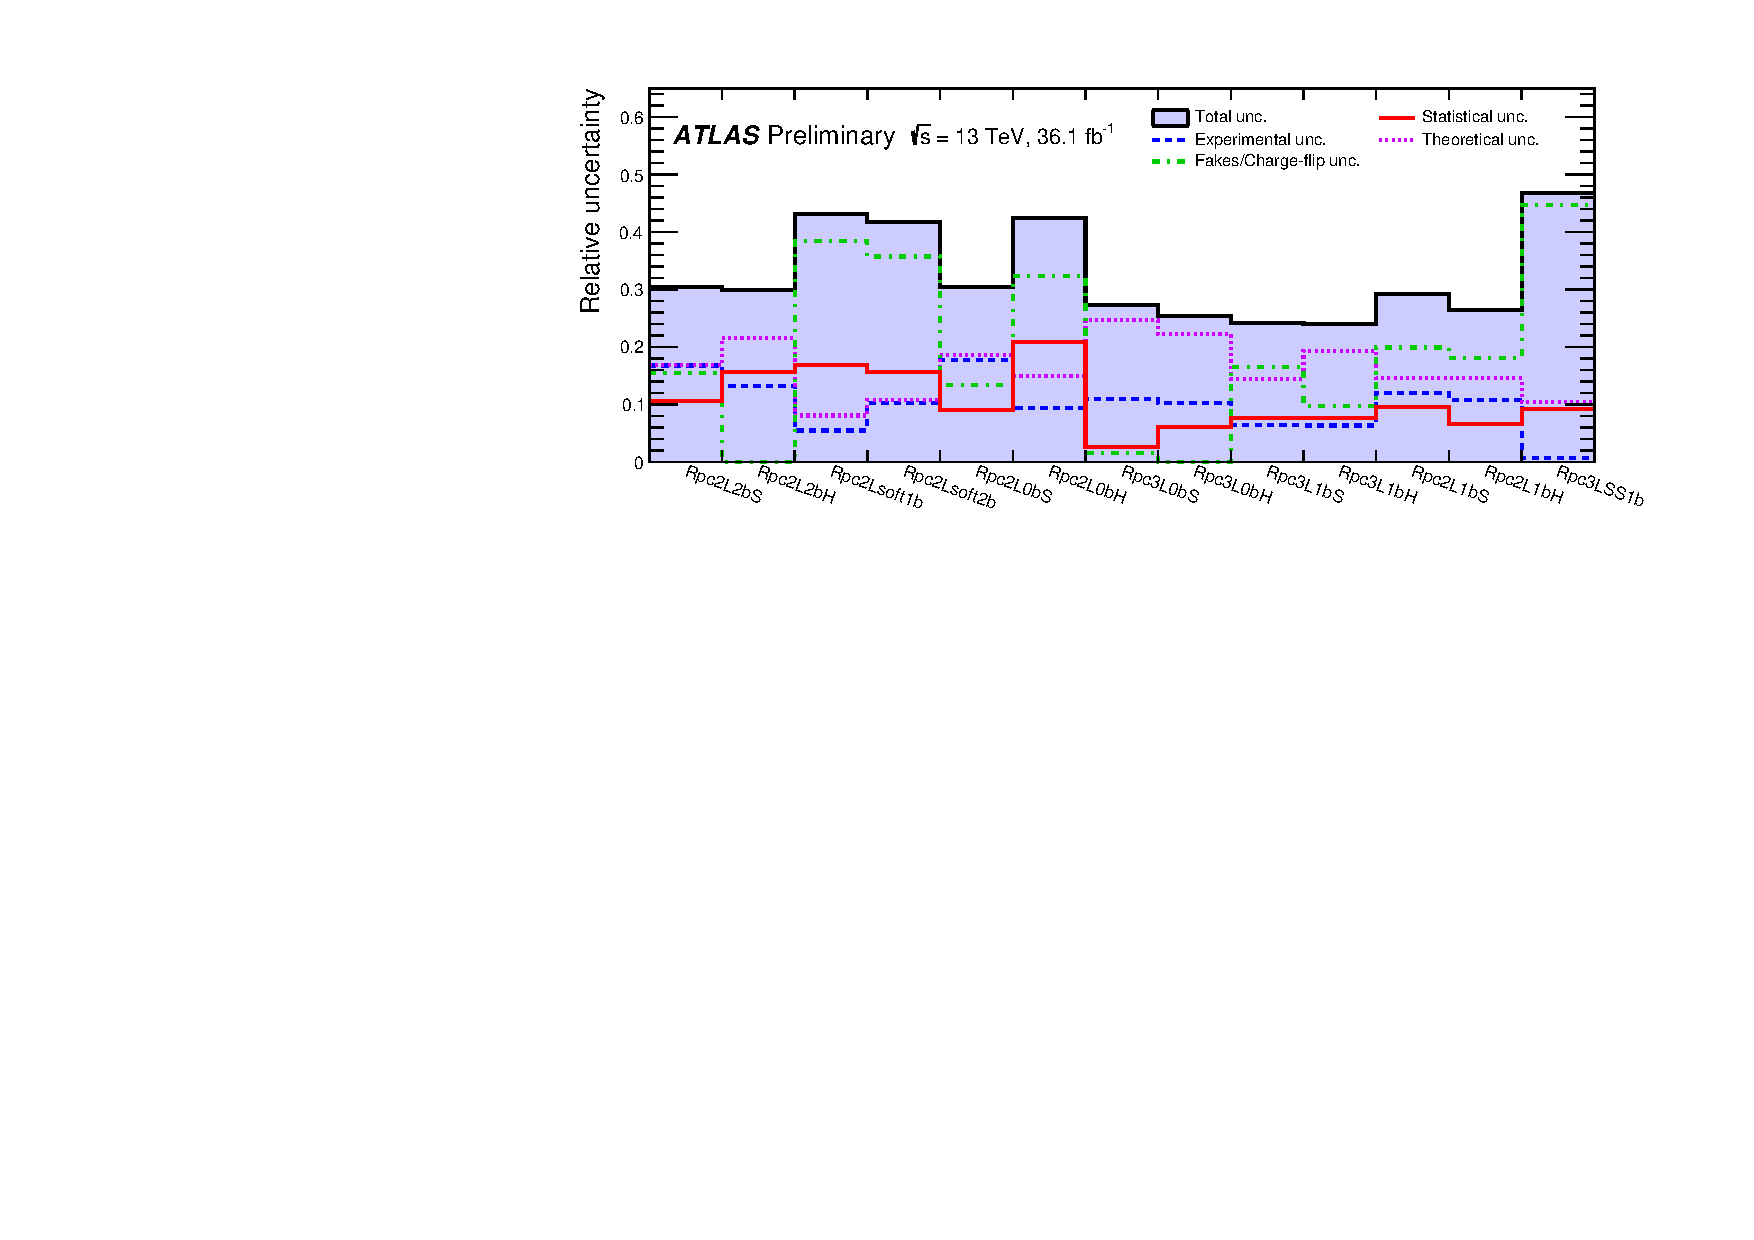
\includegraphics[width=\textwidth]{SystematicsSummary}\caption{}\end{subfigure} \\
\begin{subfigure}[t]{0.87\textwidth}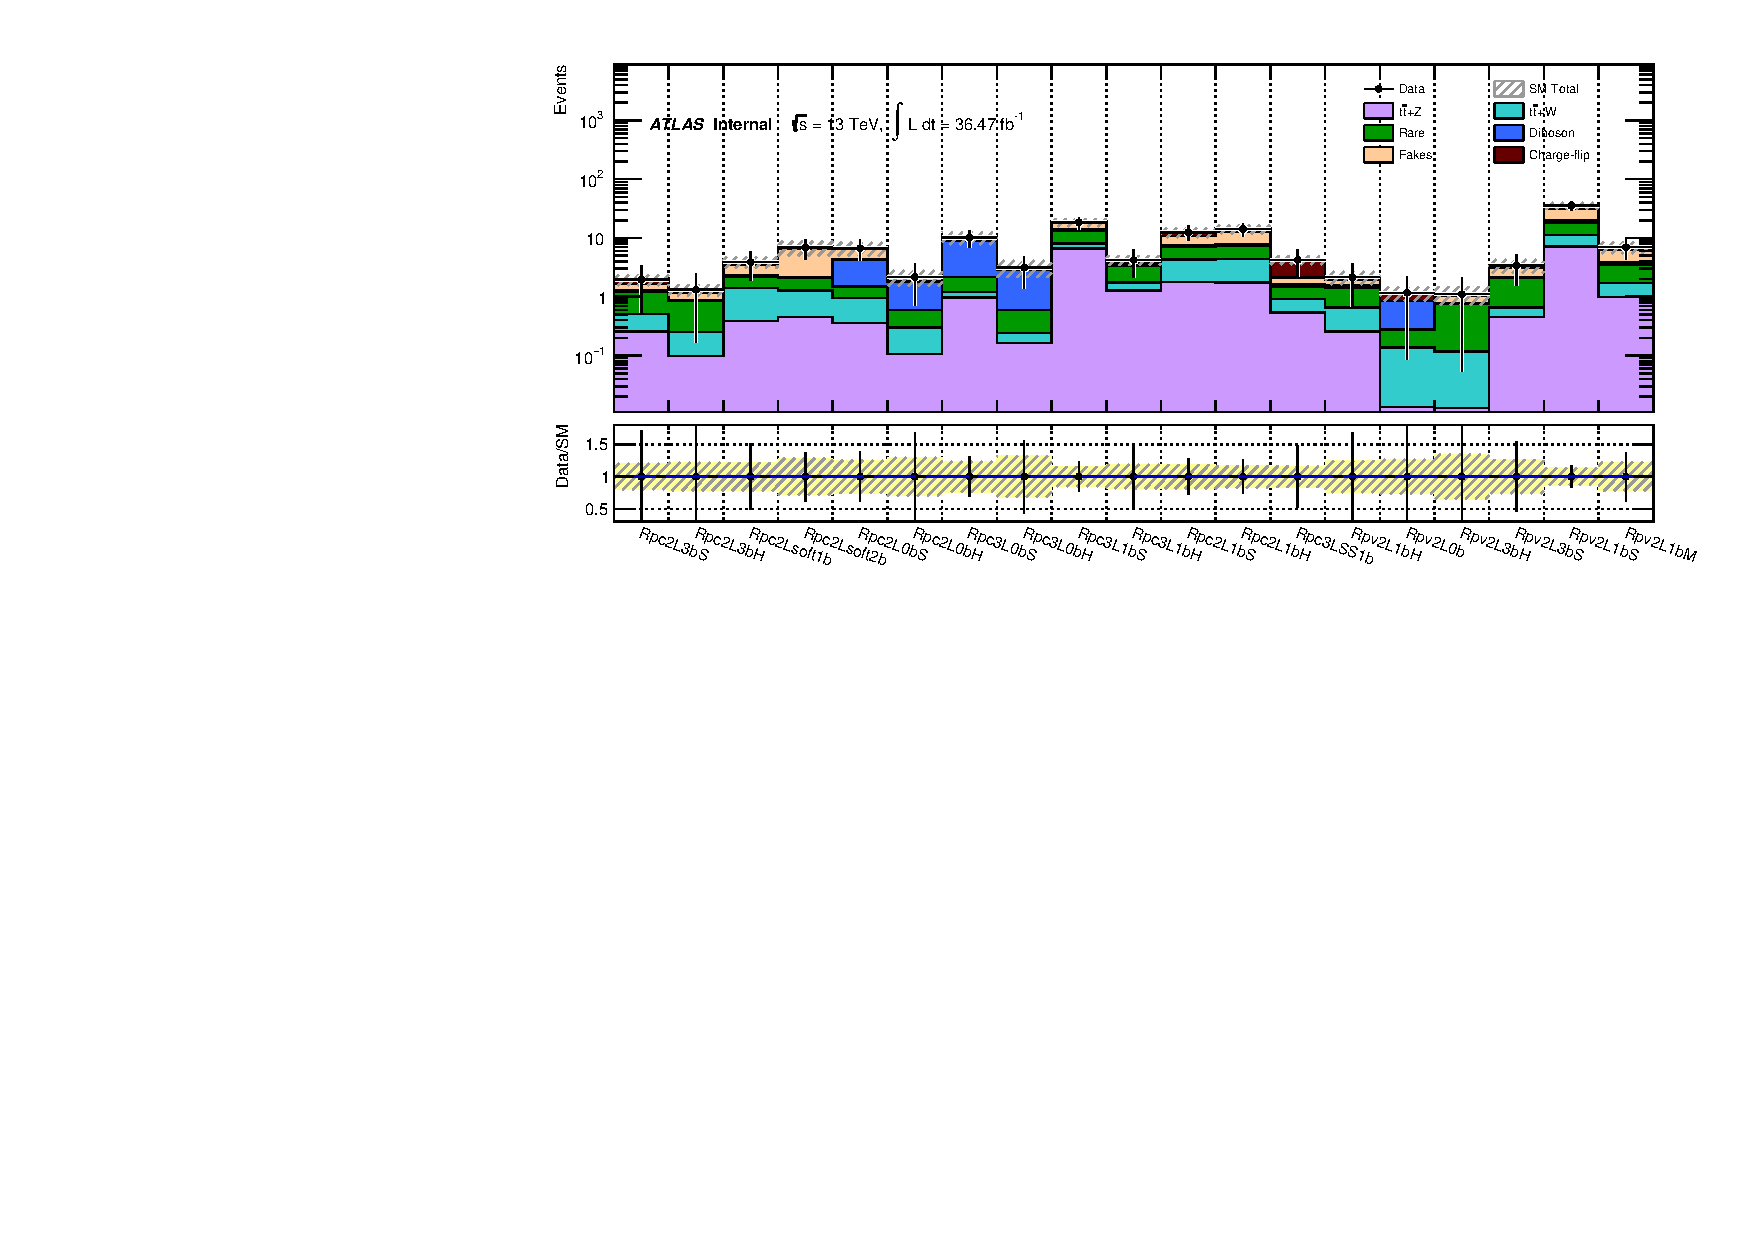
\includegraphics[width=\textwidth]{SRsummary}\caption{}\end{subfigure}
\end{center}
\caption{Relative systematic uncertainties and comparison of the observed and expected event yields in each signal region. 
The background expectations are those obtained from the background-only fits, presented in Table~\ref{tab:SR_yields}. 
\textcolor{red}{[UPDATE: Put all signal regions with final notations. Add ratio plot below SR Event Yields]}} 
\label{fig:PlotSR}
\end{figure}

%\begin{table}[h!]
%\begin{center}
%\caption{The main sources of systematic uncertainty on the SM background estimates for the four signal regions are shown 
%and their values given as relative uncertainties in the expected signal region background event yields. 
%The individual components can be correlated and therefore do not necessarily add up in quadrature to the total systematic uncertainty.
%For reference, the total number of expected background events is also shown.
%}
%\label{tab:SR_syst}
%{\small
%\begin{tabular}{lrrrr}
%\noalign{\smallskip}\hline\hline\noalign{\smallskip}
%         & SR0b3j         & SR0b5j     & SR1b & SR3b     \\[-0.05cm]
%\noalign{\smallskip}\hline\hline\noalign{\smallskip}
%Diboson theoretical uncertainties    & 23\%  &  16\%   &  1\%  &$<$1\%   \\
%$\ttbar V$ theoretical uncertainties & 3\%   &  4\%    & 13\%  &  9\%   \\
%Other theoretical uncertainties      & 5\%   &  3\%    &  9\%  & 15\%   \\
%\noalign{\smallskip}\hline\noalign{\smallskip}
%MC statistical uncertainties         & 11\%  &  14\%   &  3\%  &  6\%   \\
%\noalign{\smallskip}\hline\noalign{\smallskip}
%Jet energy scale        & 12\%   &  11\%  & 6\%    & 5\%   \\
%Jet energy resolution   & 3\%    &  9\%   & 2\%    & 3\%   \\
%$b$-tagging             & 4\%    &  6\%   & 3\%    & 10\%   \\
%PDF                     & 6\%    &  6\%   & 6\%    & 8\%   \\
%Fake/non-prompt leptons & 18\%    &  20\%   & 18\%   & 21\%   \\
%Charge flip             & --     & 1\% & 3\%    & 8\%   \\
%\noalign{\smallskip}\hline\noalign{\smallskip}
%Total background uncertainties & 30\%   & 34\%   & 22\%   & 31\%   \\
%\noalign{\smallskip}\hline\hline\noalign{\smallskip}
%Total background events & $1.5$ & $0.88$ & $4.5$ & $0.80$\\
%\noalign{\smallskip}\hline\hline\noalign{\smallskip}
%\end{tabular}
%}
%\end{center}
%\end{table}
	



%-------------------------------------------------------------------------------
\section{Results}
\label{sec:result}
%-------------------------------------------------------------------------------

\begin{table}[htb!]
\begin{center}
\setlength{\tabcolsep}{0.0pc}
\caption{The number of observed data events and expected background contributions in the signal regions. 
The $p$-value of the observed events for the background-only hypothesis is denoted by $p(s = 0)$. 
The ``Rare'' category contains the contributions from associated production of $\ttbar$ with $h/WW/t/\ttbar$, 
as well as $tZ$, $Wh$, $Zh$, and triboson production. 
Background categories shown as ``$-$'' denote that they cannot contribute to a given region (charge flips or $W^\pm W^\pm jj$ in 3-lepton regions). 
The individual uncertainties can be correlated and therefore do not necessarily add up in quadrature to the total systematic uncertainty. 
}
\label{tab:SR_yields}
{\small
\begin{tabular*}{\textwidth}{@{\extracolsep{\fill}}lcccc}
\noalign{\smallskip}\hline\hline\noalign{\smallskip}
         & SR0b3j         & SR0b5j     & SR1b & SR3b     \\[-0.05cm]
\noalign{\smallskip}\hline\hline\noalign{\smallskip}
Observed events         & $3$     &  $3$  & $7$  & $1$            \\
\noalign{\smallskip}\hline\noalign{\smallskip}
Total background events & $1.5 \pm 0.4$ & $0.88 \pm 0.29$ & $4.5 \pm 1.0$ & $0.80 \pm 0.25$\\
$p(s = 0)$                &  0.13  &  0.04  &  0.15  &   0.36   \\
\noalign{\smallskip}\hline\noalign{\smallskip}
Fake/non-prompt leptons & $<0.2$ & $0.05\pm 0.18$ & $0.8 \pm 0.8$ & $0.13 \pm 0.17$\\
Charge-flip & $-$ & $0.02 \pm 0.01$ & $0.60 \pm 0.12$ & $0.19 \pm 0.06$\\
$t\bar{t}W$ & $0.02 \pm 0.01$ & $0.08 \pm 0.04$ & $1.1 \pm 0.4$ & $0.10 \pm 0.05$\\
$t\bar{t}Z$ & $0.10 \pm 0.04$ & $0.05 \pm 0.03$ & $0.92 \pm 0.31$ & $0.14 \pm 0.06$\\
$WZ$ & $1.2 \pm 0.4$ & $0.48 \pm 0.20$ & $0.18 \pm 0.11$ & $<0.02$\\
$W^\pm W^\pm jj$ & $-$ & $0.12 \pm 0.07$ & $0.03 \pm 0.02$ & $<0.01$\\
$ZZ$ & $<0.03$ & $<0.04$ & $<0.03$ & $<0.03$\\
Rare & $0.14 \pm 0.08$ & $0.07 \pm 0.05$ & $0.8 \pm 0.4$ & $0.24 \pm 0.14$\\  
\noalign{\smallskip}\hline\hline\noalign{\smallskip}
\end{tabular*}
}
\end{center}
\end{table}

\begin{figure}[t!]
\centering
\begin{subfigure}[t]{0.49\textwidth}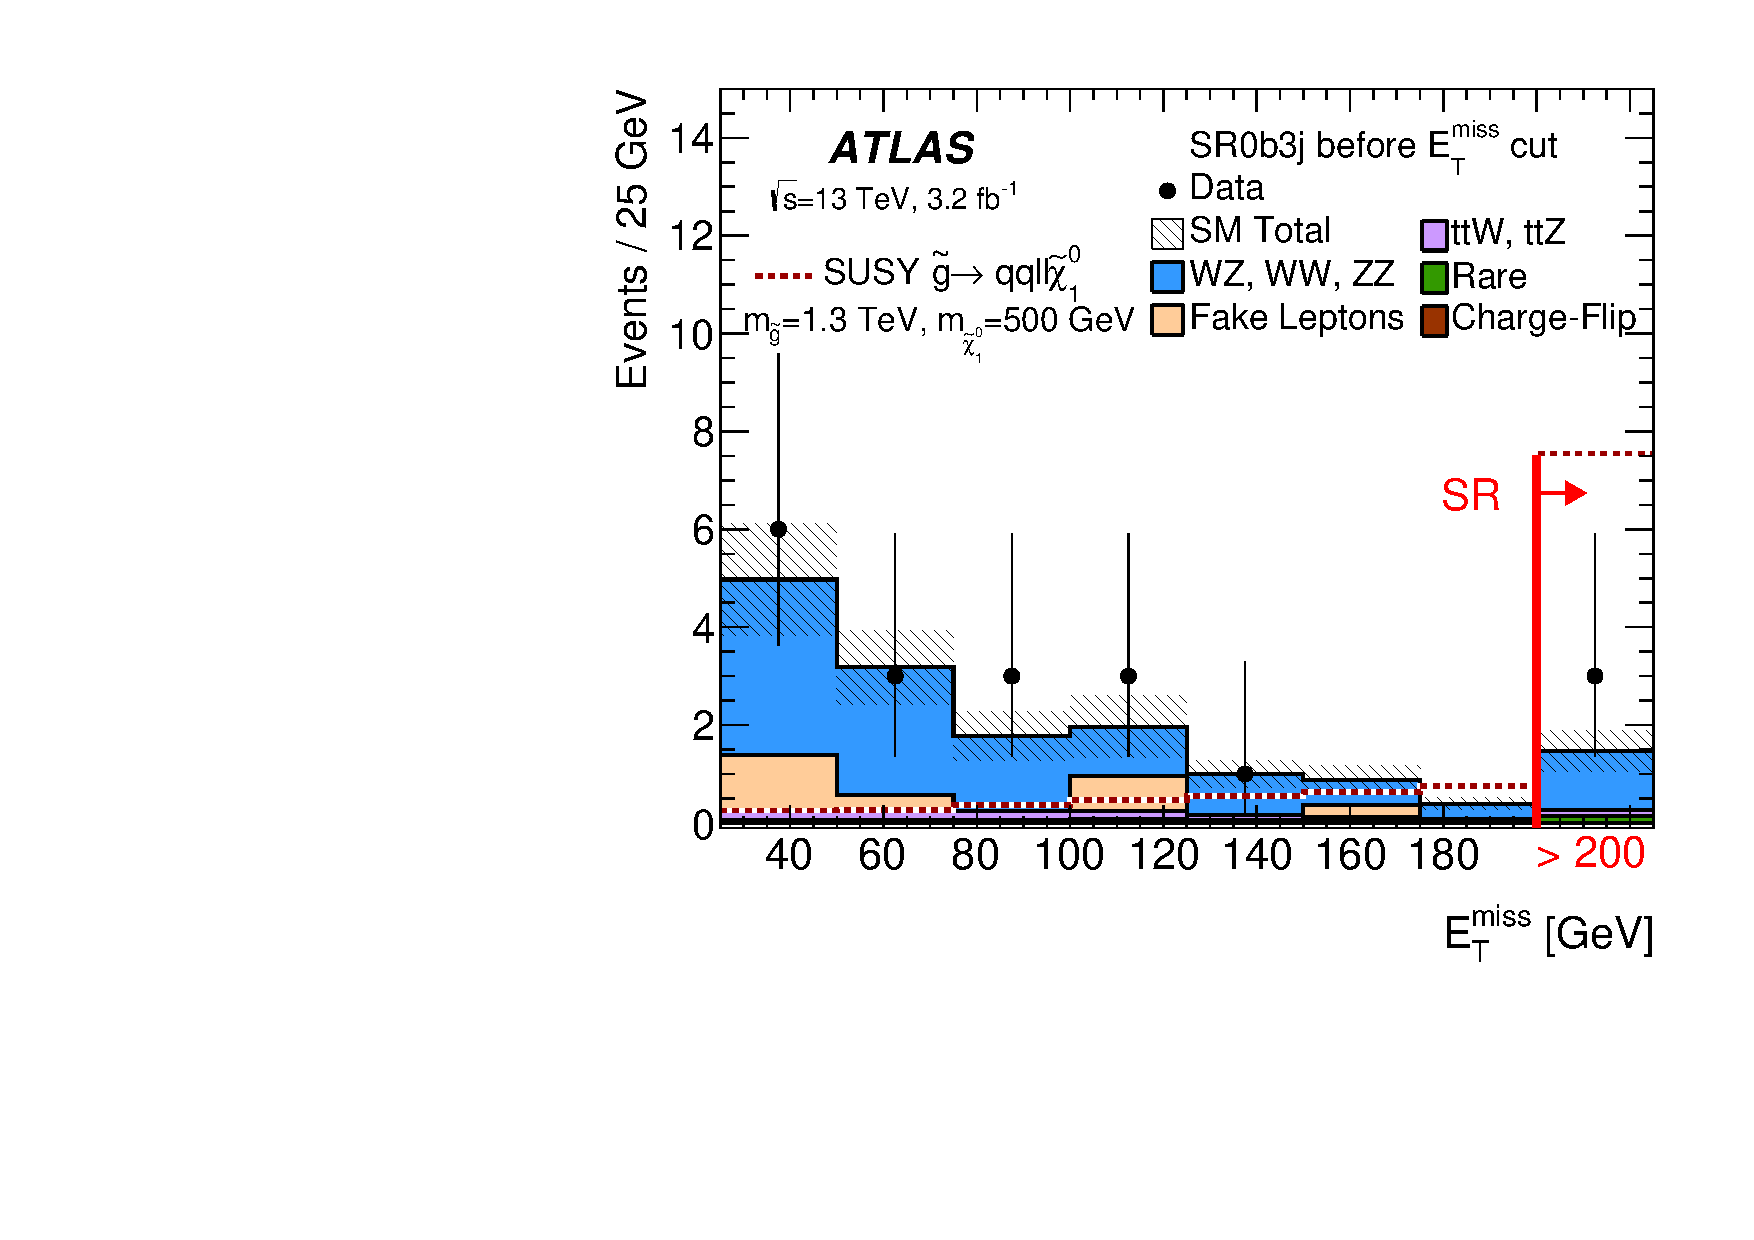
\includegraphics[width=\textwidth]{FIGURES/CONF_SR0b3j.pdf}
\caption{}\label{fig:Results_SR0b3j}\end{subfigure}
\begin{subfigure}[t]{0.49\textwidth}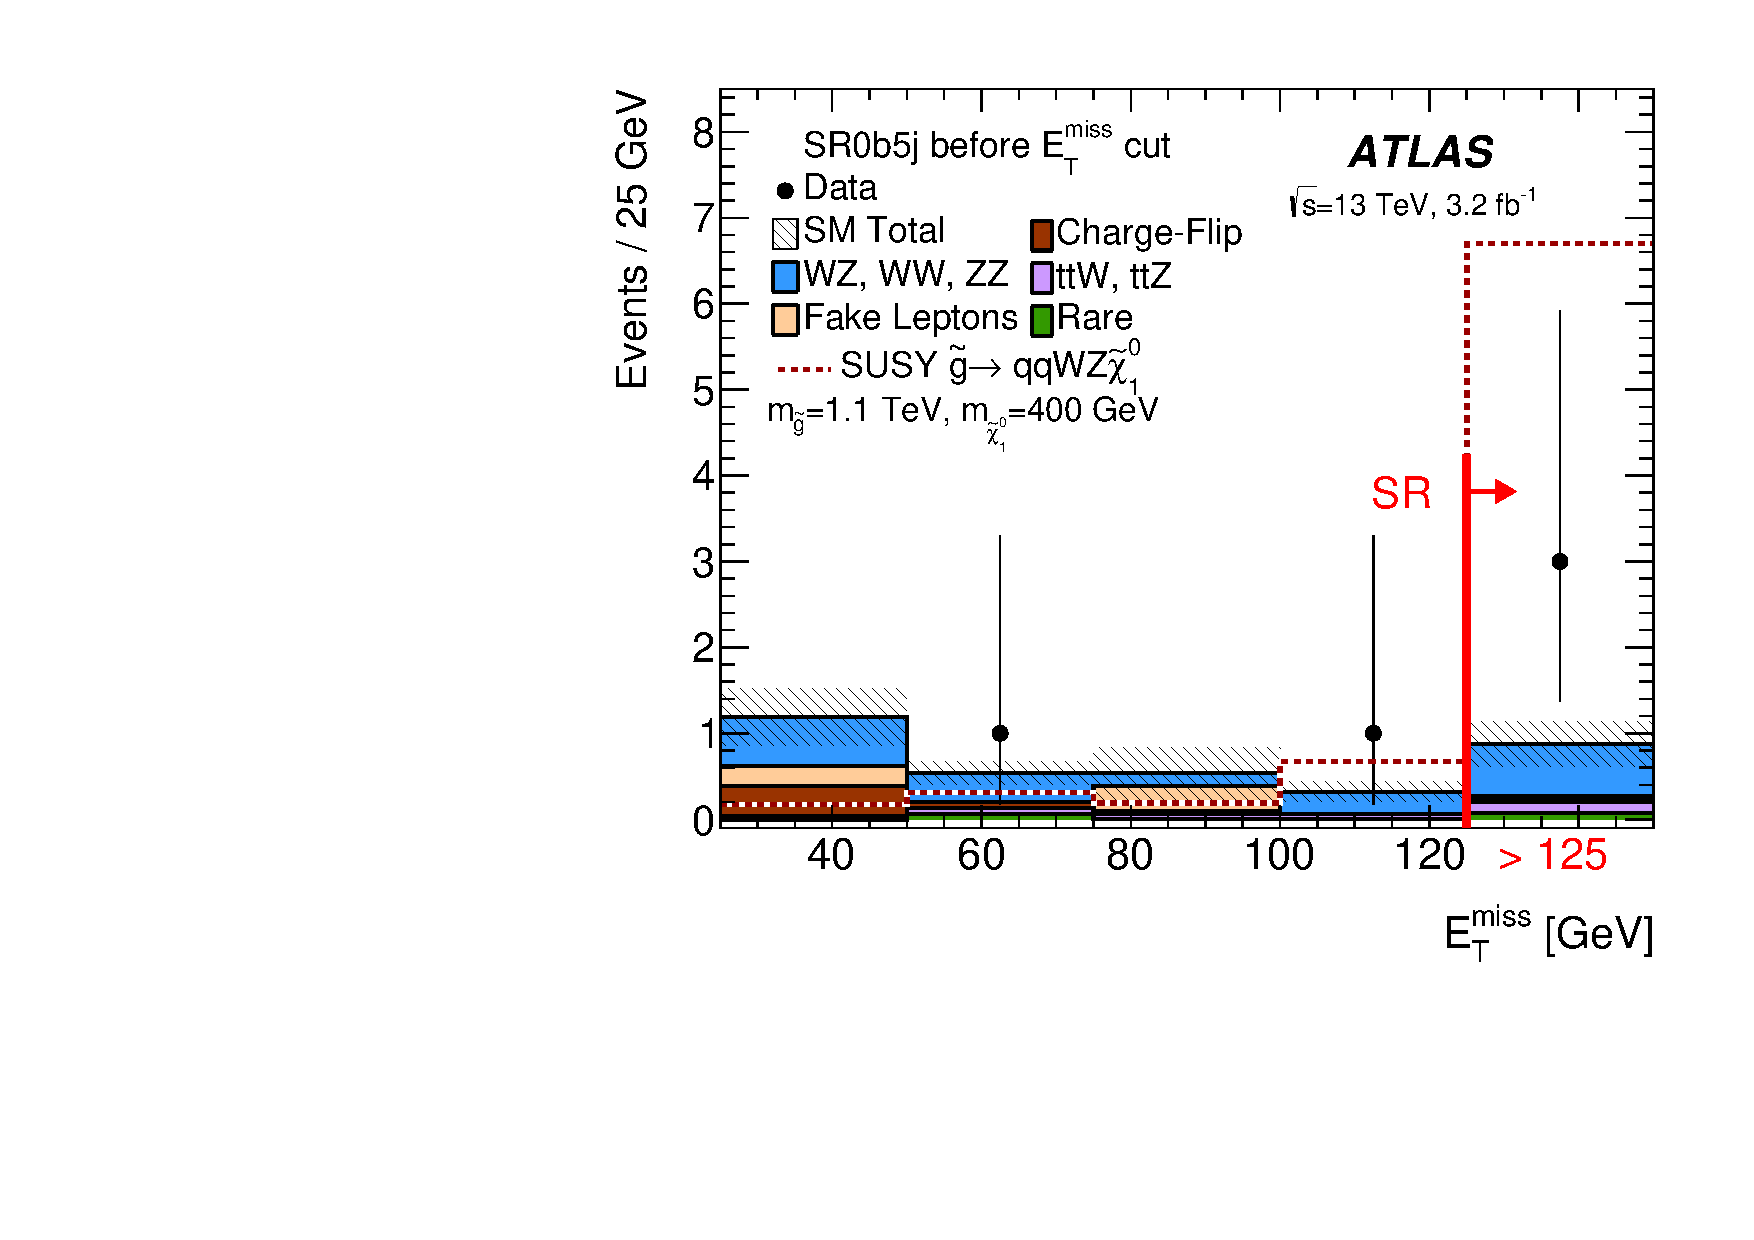
\includegraphics[width=\textwidth]{FIGURES/CONF_SR0b5j.pdf}
\caption{}\label{fig:Results_SR0b5j}\end{subfigure}
\begin{subfigure}[t]{0.49\textwidth}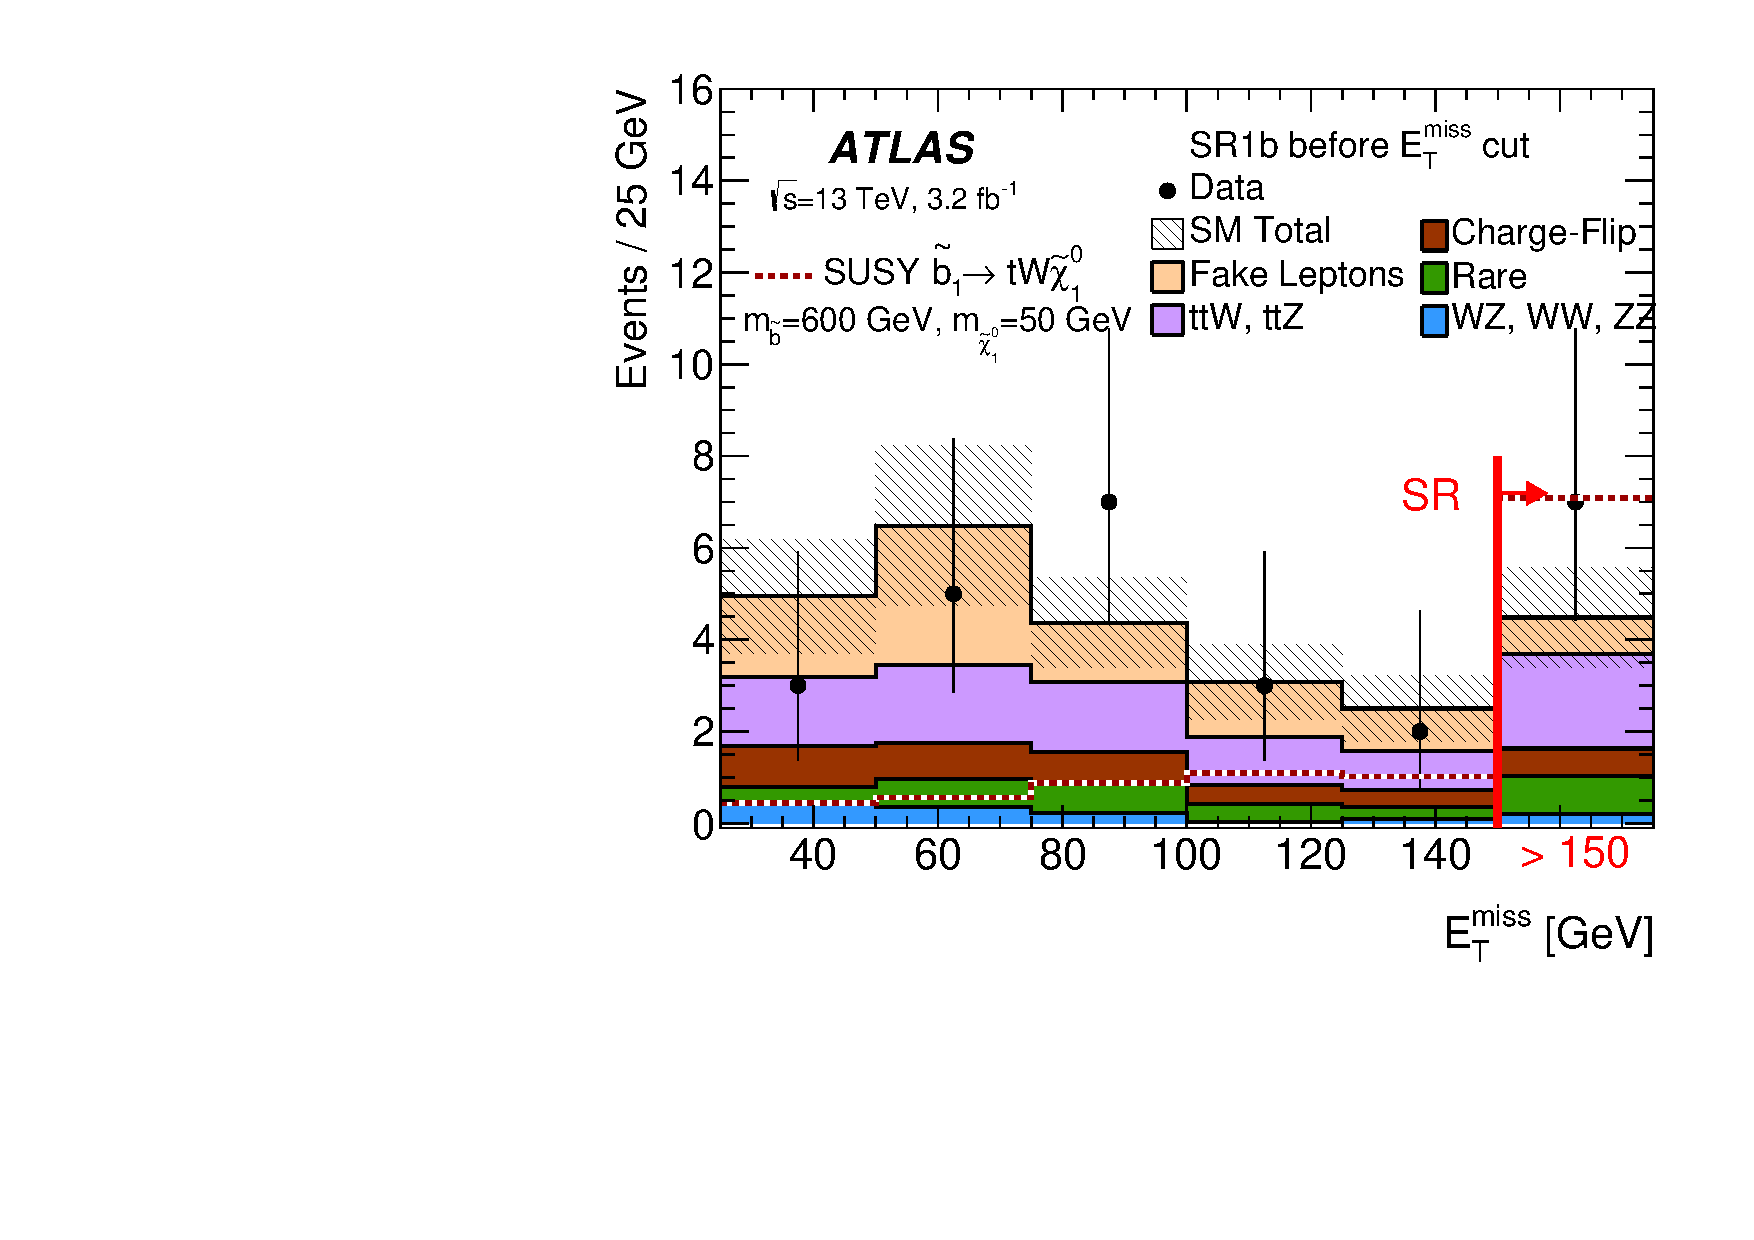
\includegraphics[width=\textwidth]{FIGURES/CONF_SR1b.pdf}
\caption{}\label{fig:Results_SR1b}\end{subfigure}
\begin{subfigure}[t]{0.49\textwidth}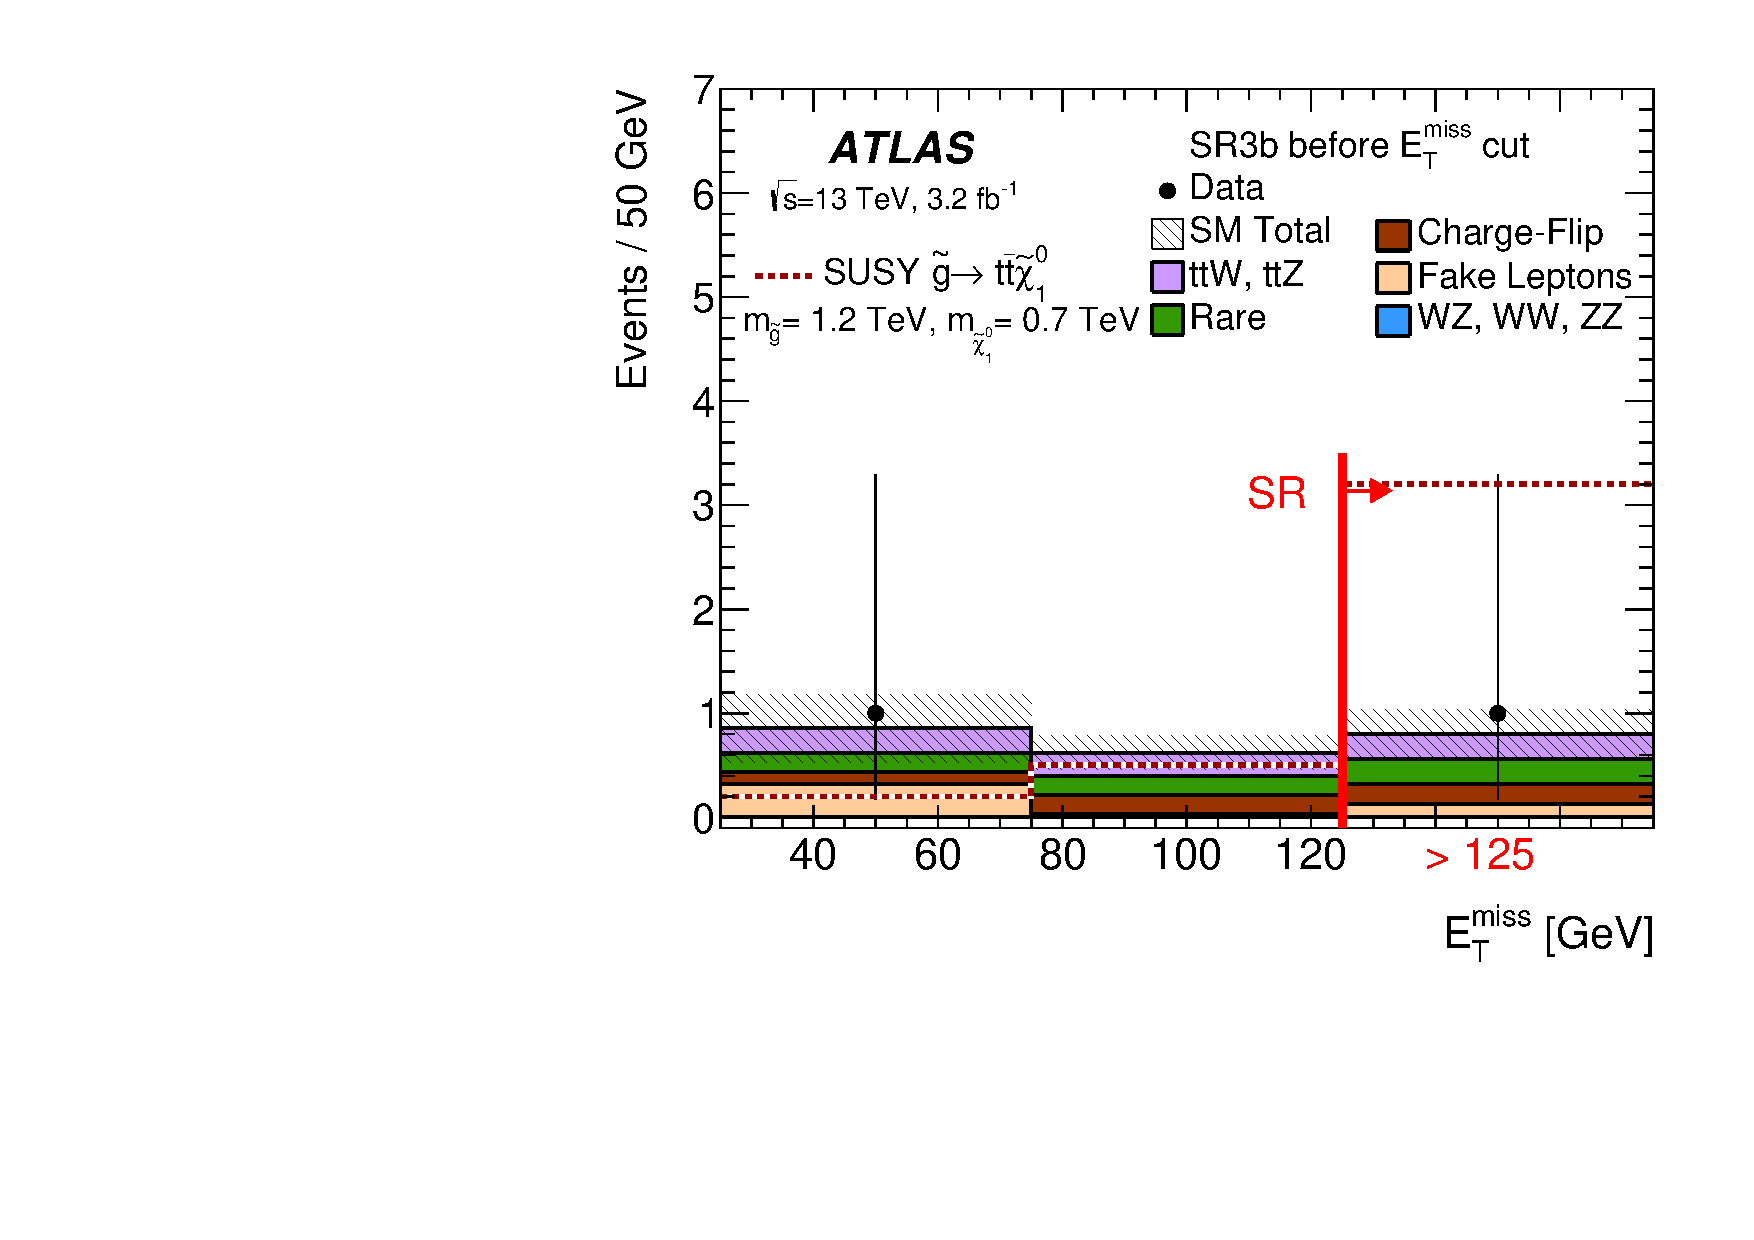
\includegraphics[width=\textwidth]{FIGURES/CONF_SR3b.pdf}
\caption{}\label{fig:Results_SR3b}\end{subfigure}
\caption{Missing transverse momentum distributions after (a) SR0b3j, (b) SR0b5j, (c) SR1b and (d) SR3b selection, beside the \met requirement. 
The results in the signal regions are shown in the last (inclusive) bin of each plot. 
The statistical uncertainties in the background prediction are included in the uncertainty band, 
as well as the theory uncertainties for the backgrounds with prompt SS/3L, 
and the full systematic uncertainties for data-driven backgrounds. 
The ``Fake leptons'' category corresponds to FNP leptons (see text), 
and the ``Rare'' category contains the contributions from associated production of $\ttbar$ with $h/WW/t/\ttbar$, 
as well as $tZ$, $Wh$, $Zh$, and triboson production. 
}
\label{fig:Results_SR_metD} 
\end{figure} 


Figure~\ref{fig:Results_SR_metD} shows the data \met distributions after the signal region selections (beside that on \met) in data 
together with the expected contributions from all the SM backgrounds with their total statistical and systematic uncertainties. 
For illustration, a typical SUSY signal distribution corresponding to the most relevant benchmark scenario 
in each SR is displayed.
The detailed yields for data and the different sources of SM background in the signal regions 
are presented in Table~\ref{tab:SR_yields}. 
The uncertainties amount to 22--34\% of the total background depending on the signal region. 
In all four SRs the number of data events exceeds the expectation but is consistent within the uncertainties, 
the smallest $p$-value for the SM-only hypothesis being 0.04 for SR0b5j. 
Out of the 14 events in the SRs, 2 of the events in SR1b and the 3 events in SR0b3j contain three leptons. 
None of those events contain three leptons of equal charge. 

In the absence of any significant deviations from the SM predictions, upper limits on possible BSM contributions to the signal regions are computed, 
in particular in the context of the SUSY benchmark scenarios described in Section~\ref{sec:intro}. 
The HistFitter framework~\cite{Baak:2014wma}, which utilises a profile-likelihood-ratio test~\cite{Cowan:2010js}, 
is used to establish 95\% confidence intervals using the CL$_\mathrm{s}$ prescription~\cite{Read_CLs}. 
The likelihood is built as the product of a Poisson probability density function describing the observed number of events in the signal region 
and Gaussian distributions constraining the nuisance parameters 
associated with the systematic uncertainties whose widths correspond to the sizes of these uncertainties; 
Poisson distributions are used instead for MC statistical uncertainties. 
Correlations of a given nuisance parameter across the different sources of backgrounds and the signal are taken into account when relevant. 
The statistical tests are performed independently for each of the signal regions. 

Table~\ref{tab:upperlimits} presents 95\% confidence level (CL) model-independent upper limits 
on the number of BSM events, $N_\mathrm{BSM}$, that may contribute to the signal regions. 
Normalising these by the integrated luminosity $L$ of the data sample, they can be interpreted as upper limits on the visible BSM cross-section $\sigma_{\rm{vis}}$, 
defined as the product $\sigma_{\rm{prod}}\times A \times\epsilon=N_\mathrm{BSM}/L$ of production cross-section, acceptance and reconstruction efficiency. 

\begin{table}[htb!]
\centering
\caption{Signal model-independent upper limits on the number of BSM events ($N_{\rm{BSM}}$) 
  and the visible signal cross-section ($\sigma_{\rm{vis}}$) in the four SRs. 
  The numbers (in parentheses) give the observed (expected under the SM hypothesis) 95\% CL upper
  limits. Calculations are performed with pseudo-experiments.
  The $\pm$1$\sigma$ variations on the expected limit due to the statistical and systematic uncertainties in the background prediction are also shown. 
}
\label{tab:upperlimits}
{\small
\renewcommand{\arraystretch}{1.4}
\begin{tabular*}{\textwidth}{@{\extracolsep{\fill}}lrrrr}
\noalign{\smallskip}\hline\hline\noalign{\smallskip}
         & SR0b3j         & SR0b5j     & SR1b & SR3b     \\[-0.05cm]
\noalign{\smallskip}\hline\hline\noalign{\smallskip}
$N_{\rm{BSM}}^{\rm{obs}}$ ($N_{\rm{BSM}}^{\rm{exp}}$) 
 & $5.9$  $({4.1}^{+1.6}_{-0.8})$
 & $6.4$ $({3.6}^{+1.2}_{-1.1})$
 & $8.8$ $({6.0}^{+2.6}_{-1.6})$ 
 & $3.8$ $({3.7}^{+1.1}_{-0.5})$ \\
$\sigma_{\rm{vis}}^{\rm{obs}}$ [fb] & 1.8 & 2.0 & 2.8 & 1.2\\
\noalign{\smallskip}\hline\hline\noalign{\smallskip}
  \end{tabular*}
}
\end{table} 

\begin{figure}[htb!]
\centering
\begin{subfigure}[t]{0.49\textwidth}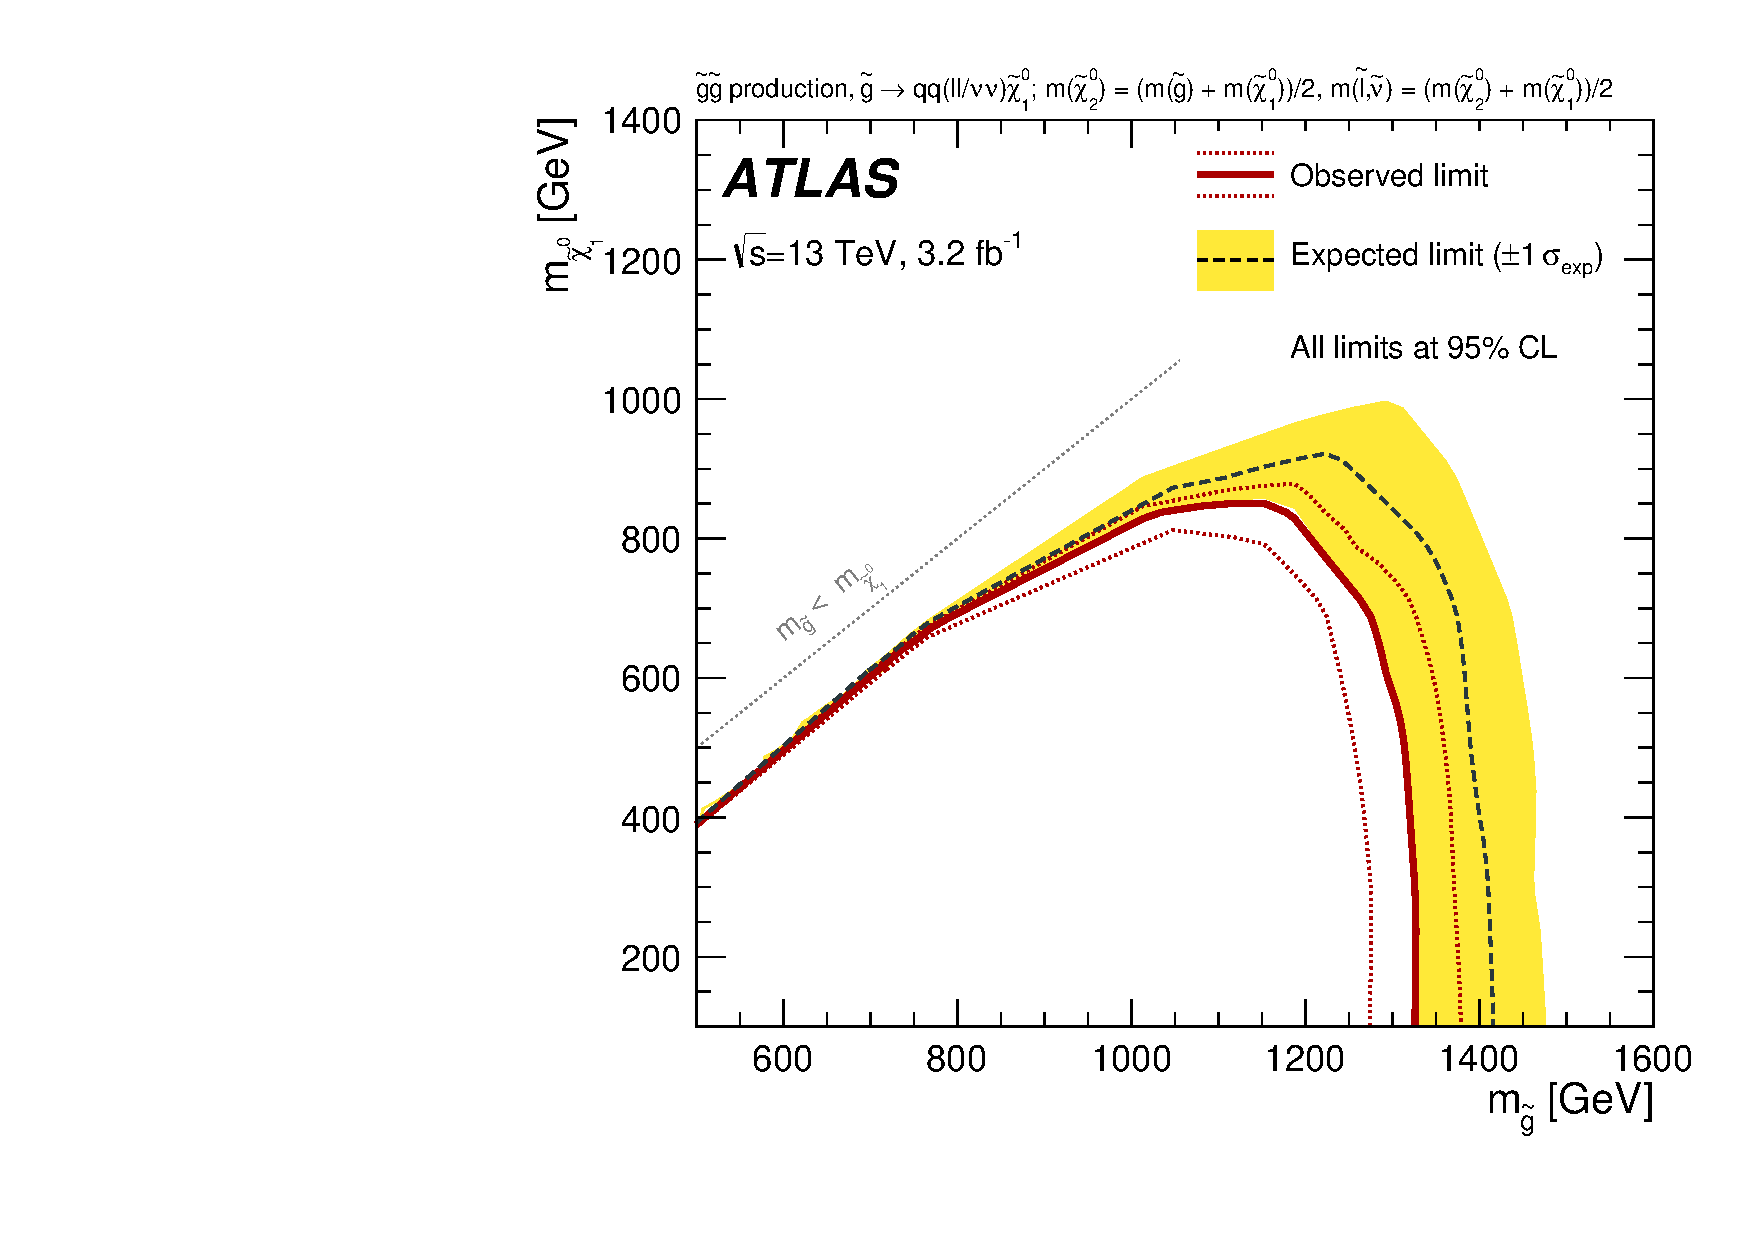
\includegraphics[width=\textwidth]{exclusion2015SameSign_SR0b3j.pdf}
\caption{$\gluino\to q\bar q \ell\ell\ninoone$ scenario, SR0b3j}\label{fig:limits_SR0b3j}\end{subfigure}
\begin{subfigure}[t]{0.49\textwidth}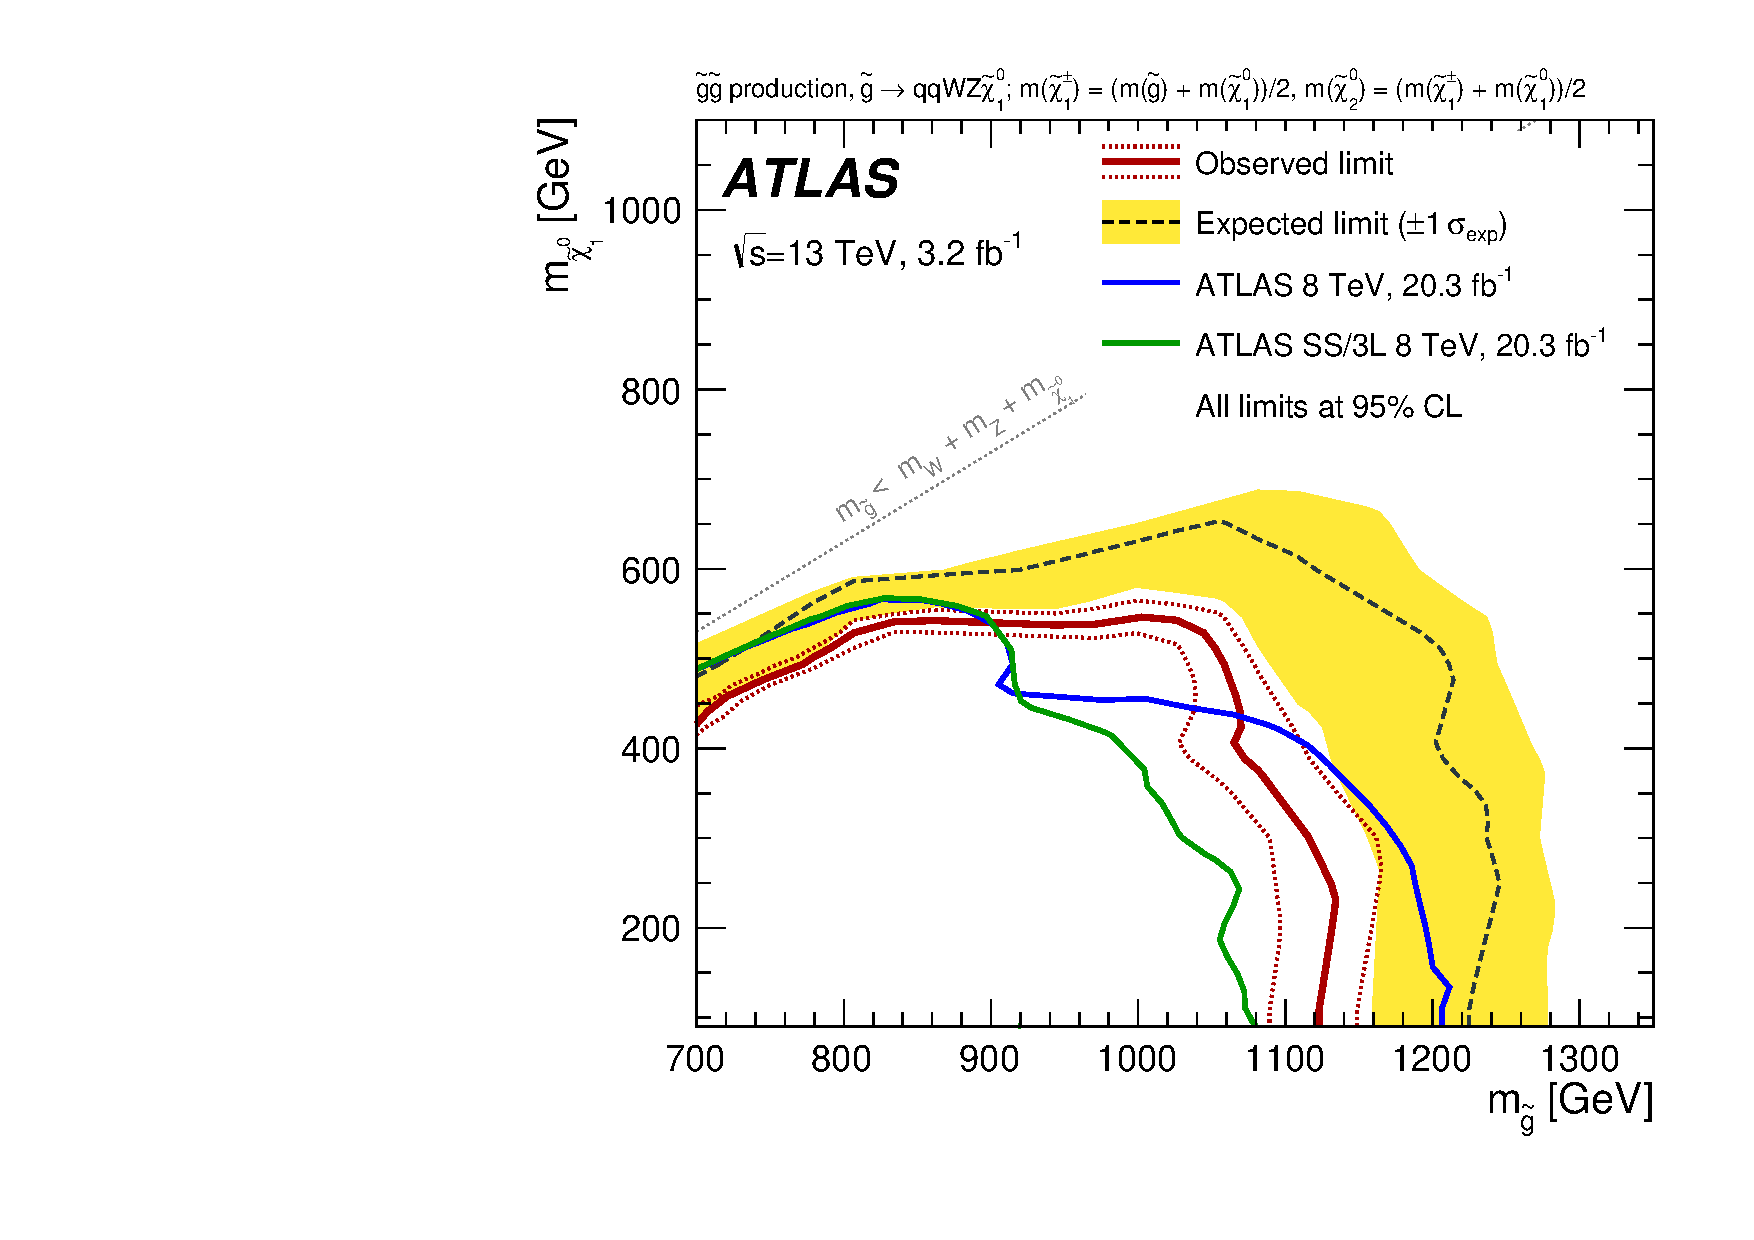
\includegraphics[width=\textwidth]{exclusion2015SameSign_SR0b5j.pdf}
\caption{$\gluino\to q\bar q' WZ\ninoone$ scenario, SR0b5j}\label{fig:limits_SR0b5j}\end{subfigure}
\par\bigskip
\begin{subfigure}[t]{0.49\textwidth}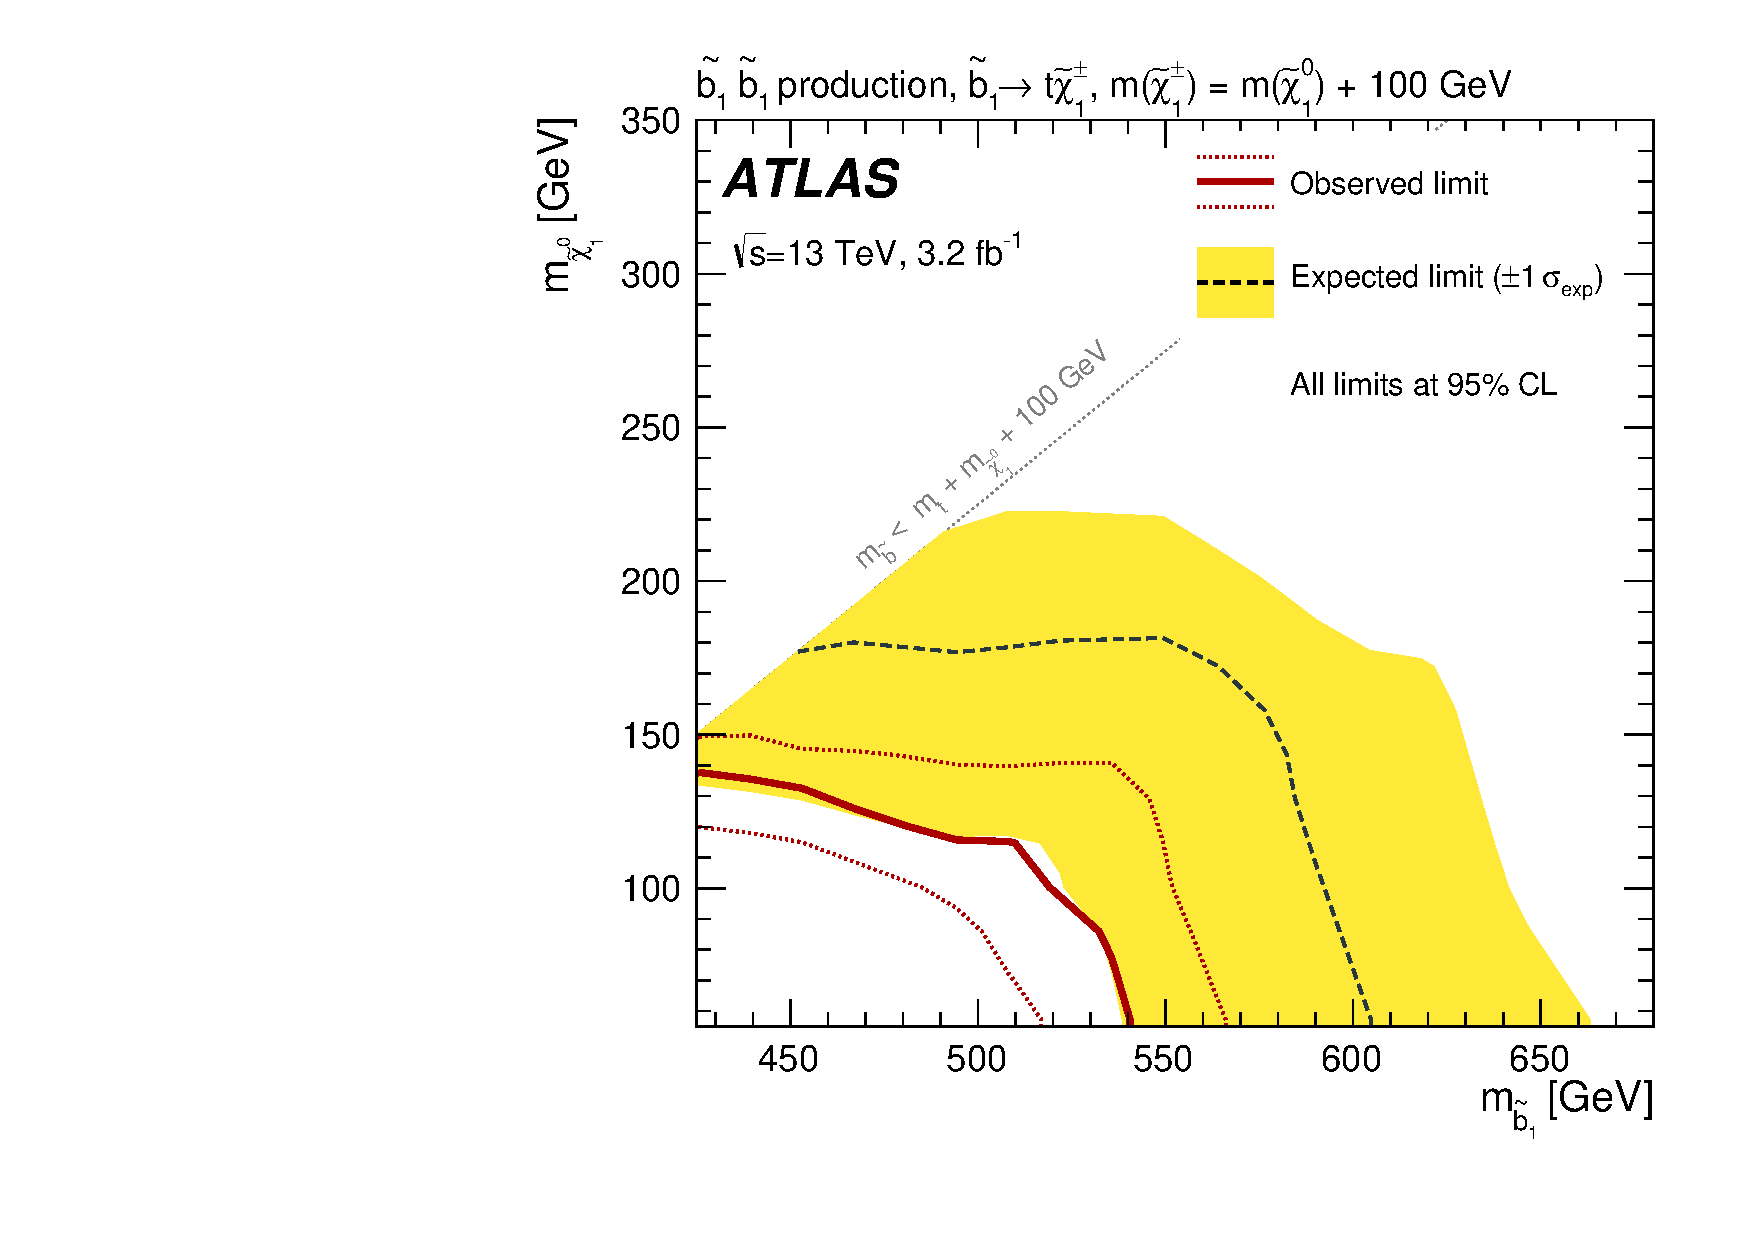
\includegraphics[width=\textwidth]{exclusion2015SameSign_SR1b.pdf}
\caption{$\sbottomone\to tW^-\ninoone$ scenario, SR1b}\label{fig:limits_SR1b}\end{subfigure}
\begin{subfigure}[t]{0.49\textwidth}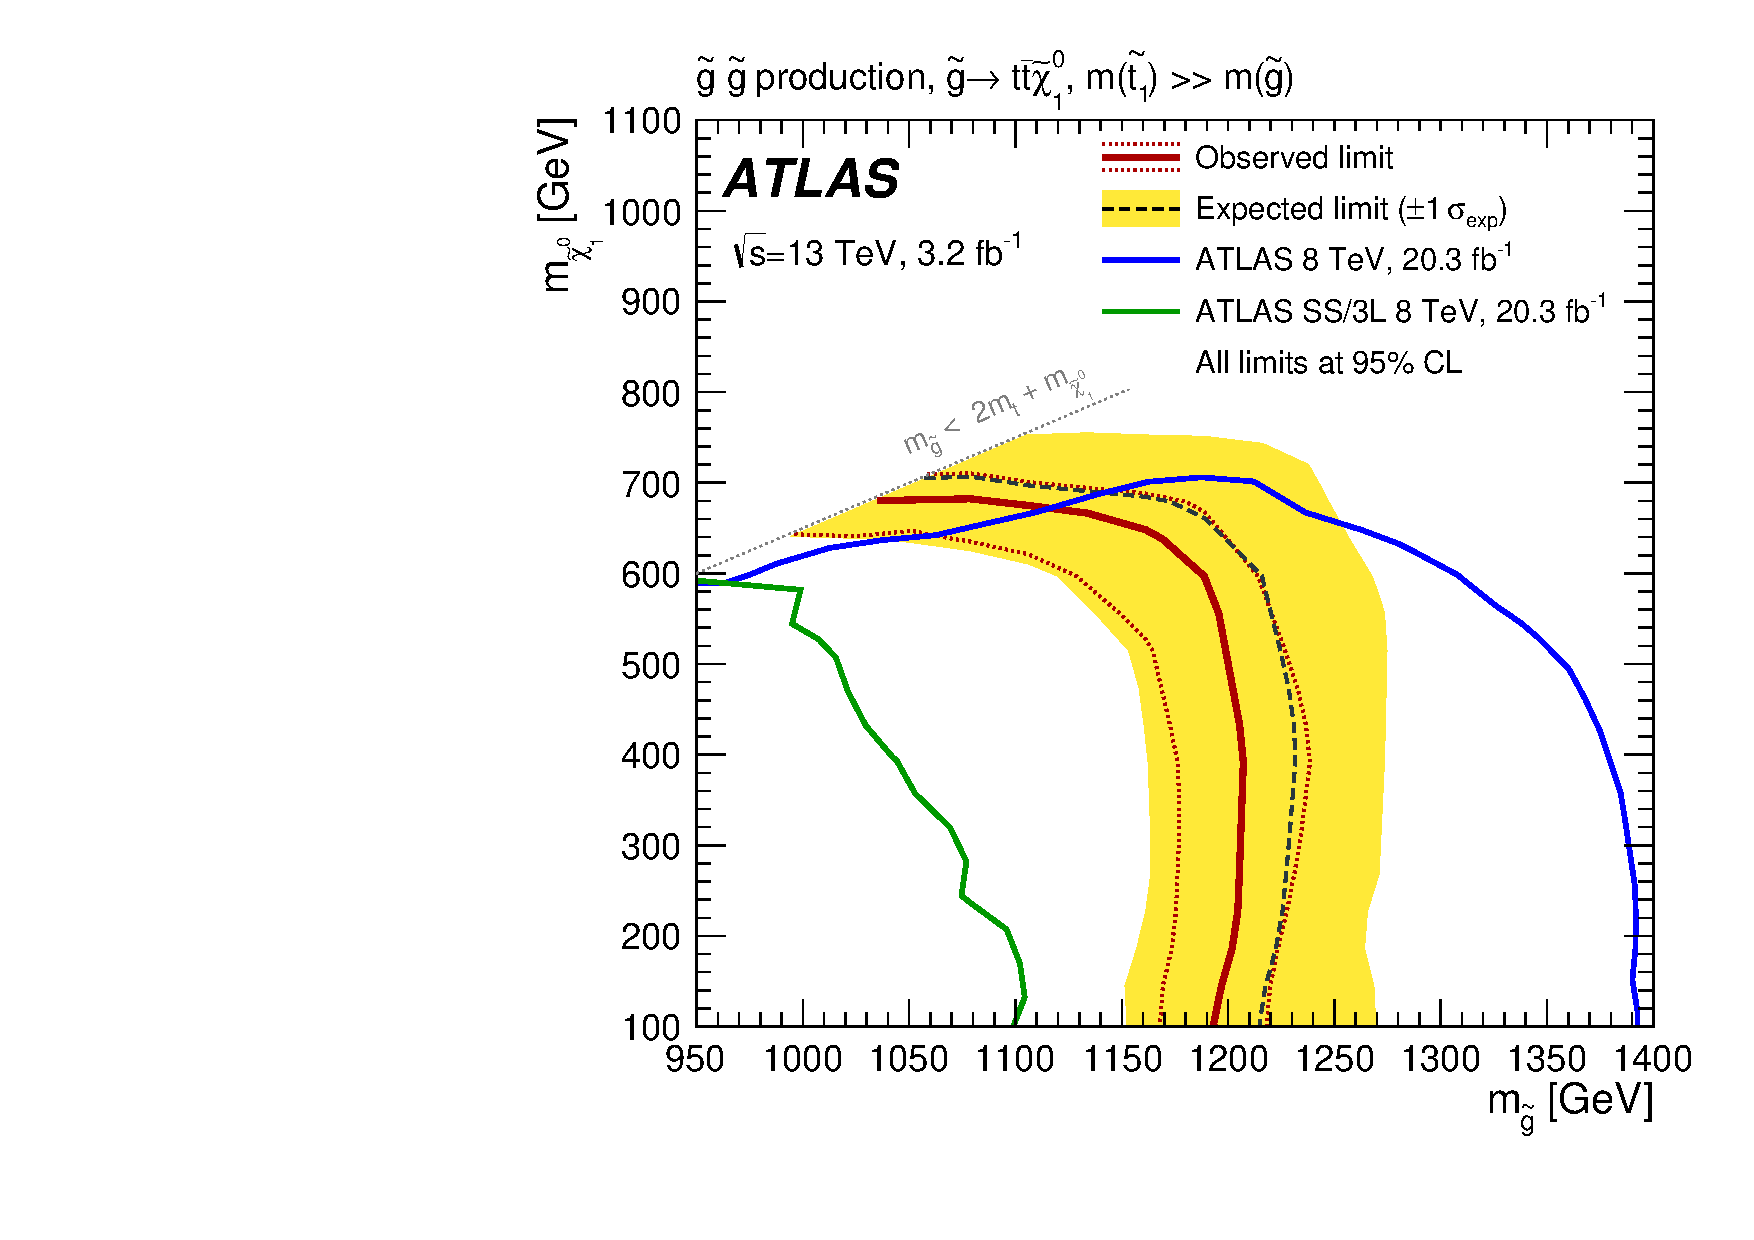
\includegraphics[width=\textwidth]{exclusion2015SameSign_SR3b.pdf}
\caption{$\gluino\to t\bar t\ninoone$ scenario, SR3b}\label{fig:limits_SR3b}\end{subfigure}
\caption{
Observed and expected exclusion limits on the \gluino, \sbottomone and \ninoone masses 
in the context of SUSY scenarios with simplified mass spectra 
featuring $\gluino\gluino$ or $\sbottomone\sbottomonebar$ pair production with exclusive decay modes. 
The signal region used to obtain the limits is specified for each scenario. 
The contours of the band around the expected limit are the $\pm$1$\sigma$ results, 
  including all uncertainties except theoretical uncertainties on the signal cross-section. The dotted lines around the observed
    limit illustrate the change in the observed limit as the nominal signal cross-section is scaled up and down
    by the theoretical uncertainty. All limits are computed at 95\% CL. 
    The diagonal lines indicate the kinematic limit for the decays in each specified scenario.  
For figures (b) and (d), results are compared with the observed limits obtained by previous ATLAS searches~\cite{paperSS3L,Aad:2015iea,Aad:2015pfx}. 
For figures (a) and (c), a direct comparison with earlier searches is not possible, due to differing model assumptions. 
}
\label{fig:Results_Limits} 
\end{figure} 

Exclusion limits are also set on the masses of the superpartners involved in the four SUSY benchmark scenarios considered in this analysis. 
Simplified models corresponding to a single production mode and with 100\% branching ratio to a specific decay chain are used, 
with the masses of the SUSY particles not involved in the process set to very high values. 
Figure~\ref{fig:Results_Limits} shows the limits 
on the mass of the $\ninoone$ as a function of the $\gluino$ or $\sbottomone$ mass. 
%For these results, asymptotic formulas~\cite{Cowan:2010js} are used to model the probability distribution of the test statistic. 
In some cases, the new limits set by this analysis can be compared 
with the existing limits set by the combination of ATLAS SUSY searches with 8 TeV data~\cite{Aad:2015iea,Aad:2015pfx}. 
For parts of the parameter space, the sensitivity reached with the 13 TeV dataset exceeds that of the 8 TeV dataset,
and additional parameter space regions can be excluded, especially for large neutralino masses. 

Signal models featuring gluino pair production with a subsequent gluino decay via $\ninotwo$ and light sleptons\\ 
($\gluino\to q\bar q\ninotwo\to q\bar q (\ell\slepton^*/\nu\tilde{\nu}^*)\to q\bar q(\ell^+\ell^-/\nu\nu)\ninoone$) 
are probed using SR0b3j (Fig.~\ref{fig:limits_SR0b3j}).
In this simplified model, the gluinos decay into $u\bar u$, $d\bar d$, $s\bar s$ or $c\bar c$ with equal probabilities, 
and the six types of leptons are also produced in the $\tilde\chi_2^0$ decays with equal probabilities. 
The $\ninotwo$ mass is set to $m_{\ninotwo}=(m_{\gluino} + m_{\ninoone})/2$, 
with the $\slepton$ and $\tilde{\nu}$ masses set to $m_{\slepton,\tilde{\nu}}=(m_{\ninotwo} + m_{\ninoone})/2$.
Gluino masses up to $m_{\gluino}\approx\SI{1.3}{TeV}$ for a light \ninoone and \ninoone masses up to $m_{\ninoone}\approx\SI{850}{GeV}$ for gluinos with $m_{\gluino}\approx\SI{1.1}{TeV}$ are excluded in this scenario. 

Similarly, models with gluino production  with a subsequent two-step gluino decay via $\chinoonepm$ and $\ninotwo$\\ 
($\gluino\to q\bar q \chinoonepm \to q\bar q W\ninotwo \to  q\bar q W Z \ninoone$) 
are probed with SR0b5j (Fig.~\ref{fig:limits_SR0b5j}).
In this simplified model, the gluinos decay into $u\bar u$, $d\bar d$, $s\bar s$ or $c\bar c$ with equal probabilities. 
The $\chinoonepm$ mass is set to $m_{\chinoonepm}=(m_{\gluino} + m_{\ninoone})/2$ and
the $\ninotwo$ mass is set to $m_{\ninotwo}=(m_{\chinoonepm} + m_{\ninoone})/2$; 
$W$ and $Z$ bosons produced in the decay chain are not necessarily on-shell. 
The exclusion limits in this scenario reach $m_{\gluino}\approx\SI{1.1}{TeV}$ (for light $\ninoone$) and $m_{\ninoone}\approx\SI{550}{GeV}$ (for $m_{\gluino}\approx\SI{1.0}{TeV}$).

Exclusion limits in a simplified model of bottom squark production with chargino-mediated $\sbottomone\to tW^-\ninoone$ decays are 
obtained with SR1b (Fig.~\ref{fig:limits_SR1b}).
In this model the $\chinoonepm$ mass is set to $m_{\chinoonepm}=m_{\ninoone} + \SI{100}{GeV}$.
The limits can reach mass values of $m_{\sbottomone}\approx\SI{540}{GeV}$ for a light $\ninoone$, 
while $m_{\ninoone}\lesssim\SI{140}{GeV}$ are also excluded for $m_{\sbottomone}\approx\SI{425}{GeV}$, 
significantly extending the previous limits obtained at $\sqrt{s}=8$~TeV~\cite{Aad:2015pfx} 
which excluded $m_{\sbottomone}\lesssim\SI{470}{GeV}$ for $m_{\ninoone}\approx\SI{60}{GeV}$ for a similar model.

Finally, SR3b is used to set limits on masses in a simplified model with 
gluino pair production and $\gluino\to t\bar t\ninoone$ decays 
via an off-shell top squark (Fig.~\ref{fig:limits_SR3b}). 
In that case, gluino masses of $m_{\gluino}\lesssim\SI{1.2}{TeV}$ are excluded for $m_{\ninoone}\lesssim\SI{600}{GeV}$, 
and $\ninoone$ masses up to $m_{\ninoone}\approx\SI{680}{GeV}$ are also excluded for $m_{\gluino}\approx\SI{1.05}{TeV}$. 


\FloatBarrier

%-------------------------------------------------------------------------------
\section{Conclusion}
\label{sec:conclusion}
%-------------------------------------------------------------------------------

A search for supersymmetry in events with exactly two same-sign leptons or at least three leptons, multiple jets, 
$b$-jets and $\met$ is presented. 
The analysis is performed with proton--proton collision data at $\sqrt{s}=13\TeV$ collected with the ATLAS detector at the Large Hadron Collider corresponding to an integrated luminosity of 3.2~fb$^{-1}$. 
With no significant excess over the Standard Model expectation observed,
results are interpreted in the framework of simplified models featuring gluino and bottom squark production.
In the $\gluino\gluino$ simplified models considered, $m_{\gluino}\lesssim 1.1$--$1.3~\TeV$ and $m_{\ninoone}\lesssim 550$--$850~\GeV$ 
are excluded at 95\% confidence level depending on the model parameters. Bottom squark masses of $m_{\sbottomone}\lesssim 540~\GeV$ 
are also excluded for a light $\ninoone$ in a $\sbottomone\sbottomonebar$ simplified model with $\sbottomone\to tW^-\ninoone$.
These results are complementary to those of previous searches and extend the exclusion limits they set.


%-------------------------------------------------------------------------------
\section*{Acknowledgements}
%-------------------------------------------------------------------------------

% Acknowledgements for papers with collision data
% Version 7-Feb-2016

% Standard acknowledgements start here
%----------------------------------------------
We thank CERN for the very successful operation of the LHC, as well as the
support staff from our institutions without whom ATLAS could not be
operated efficiently.

We acknowledge the support of ANPCyT, Argentina; YerPhI, Armenia; ARC, Australia; BMWFW and FWF, Austria; ANAS, Azerbaijan; SSTC, Belarus; CNPq and FAPESP, Brazil; NSERC, NRC and CFI, Canada; CERN; CONICYT, Chile; CAS, MOST and NSFC, China; COLCIENCIAS, Colombia; MSMT CR, MPO CR and VSC CR, Czech Republic; DNRF and DNSRC, Denmark; IN2P3-CNRS, CEA-DSM/IRFU, France; GNSF, Georgia; BMBF, HGF, and MPG, Germany; GSRT, Greece; RGC, Hong Kong SAR, China; ISF, I-CORE and Benoziyo Center, Israel; INFN, Italy; MEXT and JSPS, Japan; CNRST, Morocco; FOM and NWO, Netherlands; RCN, Norway; MNiSW and NCN, Poland; FCT, Portugal; MNE/IFA, Romania; MES of Russia and NRC KI, Russian Federation; JINR; MESTD, Serbia; MSSR, Slovakia; ARRS and MIZ\v{S}, Slovenia; DST/NRF, South Africa; MINECO, Spain; SRC and Wallenberg Foundation, Sweden; SERI, SNSF and Cantons of Bern and Geneva, Switzerland; MOST, Taiwan; TAEK, Turkey; STFC, United Kingdom; DOE and NSF, United States of America. In addition, individual groups and members have received support from BCKDF, the Canada Council, CANARIE, CRC, Compute Canada, FQRNT, and the Ontario Innovation Trust, Canada; EPLANET, ERC, FP7, Horizon 2020 and Marie Sk{\l}odowska-Curie Actions, European Union; Investissements d'Avenir Labex and Idex, ANR, R{\'e}gion Auvergne and Fondation Partager le Savoir, France; DFG and AvH Foundation, Germany; Herakleitos, Thales and Aristeia programmes co-financed by EU-ESF and the Greek NSRF; BSF, GIF and Minerva, Israel; BRF, Norway; the Royal Society and Leverhulme Trust, United Kingdom.

The crucial computing support from all WLCG partners is acknowledged
gratefully, in particular from CERN and the ATLAS Tier-1 facilities at
TRIUMF (Canada), NDGF (Denmark, Norway, Sweden), CC-IN2P3 (France),
KIT/GridKA (Germany), INFN-CNAF (Italy), NL-T1 (Netherlands), PIC (Spain),
ASGC (Taiwan), RAL (UK) and BNL (USA) and in the Tier-2 facilities
worldwide.
%----------------------------------------------



\printbibliography

\clearpage

\newpage % ATLAS Collaboration author list
% Data extracted on 13-Feb-2016 for paper reference SUSY-2015-09
%\documentclass[11pt]{article}
%\usepackage{a4wide}\begin{document}
\begin{flushleft}
{\Large The ATLAS Collaboration}

\bigskip

G.~Aad$^\textrm{\scriptsize 86}$,
B.~Abbott$^\textrm{\scriptsize 113}$,
J.~Abdallah$^\textrm{\scriptsize 151}$,
O.~Abdinov$^\textrm{\scriptsize 11}$,
B.~Abeloos$^\textrm{\scriptsize 117}$,
R.~Aben$^\textrm{\scriptsize 107}$,
M.~Abolins$^\textrm{\scriptsize 91}$,
O.S.~AbouZeid$^\textrm{\scriptsize 137}$,
H.~Abramowicz$^\textrm{\scriptsize 153}$,
H.~Abreu$^\textrm{\scriptsize 152}$,
R.~Abreu$^\textrm{\scriptsize 116}$,
Y.~Abulaiti$^\textrm{\scriptsize 146a,146b}$,
B.S.~Acharya$^\textrm{\scriptsize 163a,163b}$$^{,a}$,
L.~Adamczyk$^\textrm{\scriptsize 39a}$,
D.L.~Adams$^\textrm{\scriptsize 26}$,
J.~Adelman$^\textrm{\scriptsize 108}$,
S.~Adomeit$^\textrm{\scriptsize 100}$,
T.~Adye$^\textrm{\scriptsize 131}$,
A.A.~Affolder$^\textrm{\scriptsize 75}$,
T.~Agatonovic-Jovin$^\textrm{\scriptsize 13}$,
J.~Agricola$^\textrm{\scriptsize 55}$,
J.A.~Aguilar-Saavedra$^\textrm{\scriptsize 126a,126f}$,
S.P.~Ahlen$^\textrm{\scriptsize 23}$,
F.~Ahmadov$^\textrm{\scriptsize 66}$$^{,b}$,
G.~Aielli$^\textrm{\scriptsize 133a,133b}$,
H.~Akerstedt$^\textrm{\scriptsize 146a,146b}$,
T.P.A.~{\AA}kesson$^\textrm{\scriptsize 82}$,
A.V.~Akimov$^\textrm{\scriptsize 96}$,
G.L.~Alberghi$^\textrm{\scriptsize 21a,21b}$,
J.~Albert$^\textrm{\scriptsize 168}$,
S.~Albrand$^\textrm{\scriptsize 56}$,
M.J.~Alconada~Verzini$^\textrm{\scriptsize 72}$,
M.~Aleksa$^\textrm{\scriptsize 31}$,
I.N.~Aleksandrov$^\textrm{\scriptsize 66}$,
C.~Alexa$^\textrm{\scriptsize 27b}$,
G.~Alexander$^\textrm{\scriptsize 153}$,
T.~Alexopoulos$^\textrm{\scriptsize 10}$,
M.~Alhroob$^\textrm{\scriptsize 113}$,
G.~Alimonti$^\textrm{\scriptsize 92a}$,
J.~Alison$^\textrm{\scriptsize 32}$,
S.P.~Alkire$^\textrm{\scriptsize 36}$,
B.M.M.~Allbrooke$^\textrm{\scriptsize 149}$,
B.W.~Allen$^\textrm{\scriptsize 116}$,
P.P.~Allport$^\textrm{\scriptsize 18}$,
A.~Aloisio$^\textrm{\scriptsize 104a,104b}$,
A.~Alonso$^\textrm{\scriptsize 37}$,
F.~Alonso$^\textrm{\scriptsize 72}$,
C.~Alpigiani$^\textrm{\scriptsize 138}$,
B.~Alvarez~Gonzalez$^\textrm{\scriptsize 31}$,
D.~\'{A}lvarez~Piqueras$^\textrm{\scriptsize 166}$,
M.G.~Alviggi$^\textrm{\scriptsize 104a,104b}$,
B.T.~Amadio$^\textrm{\scriptsize 15}$,
K.~Amako$^\textrm{\scriptsize 67}$,
Y.~Amaral~Coutinho$^\textrm{\scriptsize 25a}$,
C.~Amelung$^\textrm{\scriptsize 24}$,
D.~Amidei$^\textrm{\scriptsize 90}$,
S.P.~Amor~Dos~Santos$^\textrm{\scriptsize 126a,126c}$,
A.~Amorim$^\textrm{\scriptsize 126a,126b}$,
S.~Amoroso$^\textrm{\scriptsize 31}$,
N.~Amram$^\textrm{\scriptsize 153}$,
G.~Amundsen$^\textrm{\scriptsize 24}$,
C.~Anastopoulos$^\textrm{\scriptsize 139}$,
L.S.~Ancu$^\textrm{\scriptsize 50}$,
N.~Andari$^\textrm{\scriptsize 108}$,
T.~Andeen$^\textrm{\scriptsize 32}$,
C.F.~Anders$^\textrm{\scriptsize 59b}$,
G.~Anders$^\textrm{\scriptsize 31}$,
J.K.~Anders$^\textrm{\scriptsize 75}$,
K.J.~Anderson$^\textrm{\scriptsize 32}$,
A.~Andreazza$^\textrm{\scriptsize 92a,92b}$,
V.~Andrei$^\textrm{\scriptsize 59a}$,
S.~Angelidakis$^\textrm{\scriptsize 9}$,
I.~Angelozzi$^\textrm{\scriptsize 107}$,
P.~Anger$^\textrm{\scriptsize 45}$,
A.~Angerami$^\textrm{\scriptsize 36}$,
F.~Anghinolfi$^\textrm{\scriptsize 31}$,
A.V.~Anisenkov$^\textrm{\scriptsize 109}$$^{,c}$,
N.~Anjos$^\textrm{\scriptsize 12}$,
A.~Annovi$^\textrm{\scriptsize 124a,124b}$,
M.~Antonelli$^\textrm{\scriptsize 48}$,
A.~Antonov$^\textrm{\scriptsize 98}$,
J.~Antos$^\textrm{\scriptsize 144b}$,
F.~Anulli$^\textrm{\scriptsize 132a}$,
M.~Aoki$^\textrm{\scriptsize 67}$,
L.~Aperio~Bella$^\textrm{\scriptsize 18}$,
G.~Arabidze$^\textrm{\scriptsize 91}$,
Y.~Arai$^\textrm{\scriptsize 67}$,
J.P.~Araque$^\textrm{\scriptsize 126a}$,
A.T.H.~Arce$^\textrm{\scriptsize 46}$,
F.A.~Arduh$^\textrm{\scriptsize 72}$,
J-F.~Arguin$^\textrm{\scriptsize 95}$,
S.~Argyropoulos$^\textrm{\scriptsize 64}$,
M.~Arik$^\textrm{\scriptsize 19a}$,
A.J.~Armbruster$^\textrm{\scriptsize 31}$,
L.J.~Armitage$^\textrm{\scriptsize 77}$,
O.~Arnaez$^\textrm{\scriptsize 31}$,
H.~Arnold$^\textrm{\scriptsize 49}$,
M.~Arratia$^\textrm{\scriptsize 29}$,
O.~Arslan$^\textrm{\scriptsize 22}$,
A.~Artamonov$^\textrm{\scriptsize 97}$,
G.~Artoni$^\textrm{\scriptsize 120}$,
S.~Artz$^\textrm{\scriptsize 84}$,
S.~Asai$^\textrm{\scriptsize 155}$,
N.~Asbah$^\textrm{\scriptsize 43}$,
A.~Ashkenazi$^\textrm{\scriptsize 153}$,
B.~{\AA}sman$^\textrm{\scriptsize 146a,146b}$,
L.~Asquith$^\textrm{\scriptsize 149}$,
K.~Assamagan$^\textrm{\scriptsize 26}$,
R.~Astalos$^\textrm{\scriptsize 144a}$,
M.~Atkinson$^\textrm{\scriptsize 165}$,
N.B.~Atlay$^\textrm{\scriptsize 141}$,
K.~Augsten$^\textrm{\scriptsize 128}$,
G.~Avolio$^\textrm{\scriptsize 31}$,
B.~Axen$^\textrm{\scriptsize 15}$,
M.K.~Ayoub$^\textrm{\scriptsize 117}$,
G.~Azuelos$^\textrm{\scriptsize 95}$$^{,d}$,
M.A.~Baak$^\textrm{\scriptsize 31}$,
A.E.~Baas$^\textrm{\scriptsize 59a}$,
M.J.~Baca$^\textrm{\scriptsize 18}$,
H.~Bachacou$^\textrm{\scriptsize 136}$,
K.~Bachas$^\textrm{\scriptsize 74a,74b}$,
M.~Backes$^\textrm{\scriptsize 31}$,
M.~Backhaus$^\textrm{\scriptsize 31}$,
P.~Bagiacchi$^\textrm{\scriptsize 132a,132b}$,
P.~Bagnaia$^\textrm{\scriptsize 132a,132b}$,
Y.~Bai$^\textrm{\scriptsize 34a}$,
J.T.~Baines$^\textrm{\scriptsize 131}$,
O.K.~Baker$^\textrm{\scriptsize 175}$,
E.M.~Baldin$^\textrm{\scriptsize 109}$$^{,c}$,
P.~Balek$^\textrm{\scriptsize 129}$,
T.~Balestri$^\textrm{\scriptsize 148}$,
F.~Balli$^\textrm{\scriptsize 136}$,
W.K.~Balunas$^\textrm{\scriptsize 122}$,
E.~Banas$^\textrm{\scriptsize 40}$,
Sw.~Banerjee$^\textrm{\scriptsize 172}$$^{,e}$,
A.A.E.~Bannoura$^\textrm{\scriptsize 174}$,
L.~Barak$^\textrm{\scriptsize 31}$,
E.L.~Barberio$^\textrm{\scriptsize 89}$,
D.~Barberis$^\textrm{\scriptsize 51a,51b}$,
M.~Barbero$^\textrm{\scriptsize 86}$,
T.~Barillari$^\textrm{\scriptsize 101}$,
M.~Barisonzi$^\textrm{\scriptsize 163a,163b}$,
T.~Barklow$^\textrm{\scriptsize 143}$,
N.~Barlow$^\textrm{\scriptsize 29}$,
S.L.~Barnes$^\textrm{\scriptsize 85}$,
B.M.~Barnett$^\textrm{\scriptsize 131}$,
R.M.~Barnett$^\textrm{\scriptsize 15}$,
Z.~Barnovska$^\textrm{\scriptsize 5}$,
A.~Baroncelli$^\textrm{\scriptsize 134a}$,
G.~Barone$^\textrm{\scriptsize 24}$,
A.J.~Barr$^\textrm{\scriptsize 120}$,
L.~Barranco~Navarro$^\textrm{\scriptsize 166}$,
F.~Barreiro$^\textrm{\scriptsize 83}$,
J.~Barreiro~Guimar\~{a}es~da~Costa$^\textrm{\scriptsize 34a}$,
R.~Bartoldus$^\textrm{\scriptsize 143}$,
A.E.~Barton$^\textrm{\scriptsize 73}$,
P.~Bartos$^\textrm{\scriptsize 144a}$,
A.~Basalaev$^\textrm{\scriptsize 123}$,
A.~Bassalat$^\textrm{\scriptsize 117}$,
A.~Basye$^\textrm{\scriptsize 165}$,
R.L.~Bates$^\textrm{\scriptsize 54}$,
S.J.~Batista$^\textrm{\scriptsize 158}$,
J.R.~Batley$^\textrm{\scriptsize 29}$,
M.~Battaglia$^\textrm{\scriptsize 137}$,
M.~Bauce$^\textrm{\scriptsize 132a,132b}$,
F.~Bauer$^\textrm{\scriptsize 136}$,
H.S.~Bawa$^\textrm{\scriptsize 143}$$^{,f}$,
J.B.~Beacham$^\textrm{\scriptsize 111}$,
M.D.~Beattie$^\textrm{\scriptsize 73}$,
T.~Beau$^\textrm{\scriptsize 81}$,
P.H.~Beauchemin$^\textrm{\scriptsize 161}$,
P.~Bechtle$^\textrm{\scriptsize 22}$,
H.P.~Beck$^\textrm{\scriptsize 17}$$^{,g}$,
K.~Becker$^\textrm{\scriptsize 120}$,
M.~Becker$^\textrm{\scriptsize 84}$,
M.~Beckingham$^\textrm{\scriptsize 169}$,
C.~Becot$^\textrm{\scriptsize 110}$,
A.J.~Beddall$^\textrm{\scriptsize 19e}$,
A.~Beddall$^\textrm{\scriptsize 19b}$,
V.A.~Bednyakov$^\textrm{\scriptsize 66}$,
M.~Bedognetti$^\textrm{\scriptsize 107}$,
C.P.~Bee$^\textrm{\scriptsize 148}$,
L.J.~Beemster$^\textrm{\scriptsize 107}$,
T.A.~Beermann$^\textrm{\scriptsize 31}$,
M.~Begel$^\textrm{\scriptsize 26}$,
J.K.~Behr$^\textrm{\scriptsize 120}$,
C.~Belanger-Champagne$^\textrm{\scriptsize 88}$,
A.S.~Bell$^\textrm{\scriptsize 79}$,
G.~Bella$^\textrm{\scriptsize 153}$,
L.~Bellagamba$^\textrm{\scriptsize 21a}$,
A.~Bellerive$^\textrm{\scriptsize 30}$,
M.~Bellomo$^\textrm{\scriptsize 87}$,
K.~Belotskiy$^\textrm{\scriptsize 98}$,
O.~Beltramello$^\textrm{\scriptsize 31}$,
N.L.~Belyaev$^\textrm{\scriptsize 98}$,
O.~Benary$^\textrm{\scriptsize 153}$,
D.~Benchekroun$^\textrm{\scriptsize 135a}$,
M.~Bender$^\textrm{\scriptsize 100}$,
K.~Bendtz$^\textrm{\scriptsize 146a,146b}$,
N.~Benekos$^\textrm{\scriptsize 10}$,
Y.~Benhammou$^\textrm{\scriptsize 153}$,
E.~Benhar~Noccioli$^\textrm{\scriptsize 175}$,
J.~Benitez$^\textrm{\scriptsize 64}$,
J.A.~Benitez~Garcia$^\textrm{\scriptsize 159b}$,
D.P.~Benjamin$^\textrm{\scriptsize 46}$,
J.R.~Bensinger$^\textrm{\scriptsize 24}$,
S.~Bentvelsen$^\textrm{\scriptsize 107}$,
L.~Beresford$^\textrm{\scriptsize 120}$,
M.~Beretta$^\textrm{\scriptsize 48}$,
D.~Berge$^\textrm{\scriptsize 107}$,
E.~Bergeaas~Kuutmann$^\textrm{\scriptsize 164}$,
N.~Berger$^\textrm{\scriptsize 5}$,
F.~Berghaus$^\textrm{\scriptsize 168}$,
J.~Beringer$^\textrm{\scriptsize 15}$,
S.~Berlendis$^\textrm{\scriptsize 56}$,
N.R.~Bernard$^\textrm{\scriptsize 87}$,
C.~Bernius$^\textrm{\scriptsize 110}$,
F.U.~Bernlochner$^\textrm{\scriptsize 22}$,
T.~Berry$^\textrm{\scriptsize 78}$,
P.~Berta$^\textrm{\scriptsize 129}$,
C.~Bertella$^\textrm{\scriptsize 84}$,
G.~Bertoli$^\textrm{\scriptsize 146a,146b}$,
F.~Bertolucci$^\textrm{\scriptsize 124a,124b}$,
I.A.~Bertram$^\textrm{\scriptsize 73}$,
C.~Bertsche$^\textrm{\scriptsize 113}$,
D.~Bertsche$^\textrm{\scriptsize 113}$,
G.J.~Besjes$^\textrm{\scriptsize 37}$,
O.~Bessidskaia~Bylund$^\textrm{\scriptsize 146a,146b}$,
M.~Bessner$^\textrm{\scriptsize 43}$,
N.~Besson$^\textrm{\scriptsize 136}$,
C.~Betancourt$^\textrm{\scriptsize 49}$,
S.~Bethke$^\textrm{\scriptsize 101}$,
A.J.~Bevan$^\textrm{\scriptsize 77}$,
W.~Bhimji$^\textrm{\scriptsize 15}$,
R.M.~Bianchi$^\textrm{\scriptsize 125}$,
L.~Bianchini$^\textrm{\scriptsize 24}$,
M.~Bianco$^\textrm{\scriptsize 31}$,
O.~Biebel$^\textrm{\scriptsize 100}$,
D.~Biedermann$^\textrm{\scriptsize 16}$,
R.~Bielski$^\textrm{\scriptsize 85}$,
N.V.~Biesuz$^\textrm{\scriptsize 124a,124b}$,
M.~Biglietti$^\textrm{\scriptsize 134a}$,
J.~Bilbao~De~Mendizabal$^\textrm{\scriptsize 50}$,
H.~Bilokon$^\textrm{\scriptsize 48}$,
M.~Bindi$^\textrm{\scriptsize 55}$,
S.~Binet$^\textrm{\scriptsize 117}$,
A.~Bingul$^\textrm{\scriptsize 19b}$,
C.~Bini$^\textrm{\scriptsize 132a,132b}$,
S.~Biondi$^\textrm{\scriptsize 21a,21b}$,
D.M.~Bjergaard$^\textrm{\scriptsize 46}$,
C.W.~Black$^\textrm{\scriptsize 150}$,
J.E.~Black$^\textrm{\scriptsize 143}$,
K.M.~Black$^\textrm{\scriptsize 23}$,
D.~Blackburn$^\textrm{\scriptsize 138}$,
R.E.~Blair$^\textrm{\scriptsize 6}$,
J.-B.~Blanchard$^\textrm{\scriptsize 136}$,
J.E.~Blanco$^\textrm{\scriptsize 78}$,
T.~Blazek$^\textrm{\scriptsize 144a}$,
I.~Bloch$^\textrm{\scriptsize 43}$,
C.~Blocker$^\textrm{\scriptsize 24}$,
W.~Blum$^\textrm{\scriptsize 84}$$^{,*}$,
U.~Blumenschein$^\textrm{\scriptsize 55}$,
S.~Blunier$^\textrm{\scriptsize 33a}$,
G.J.~Bobbink$^\textrm{\scriptsize 107}$,
V.S.~Bobrovnikov$^\textrm{\scriptsize 109}$$^{,c}$,
S.S.~Bocchetta$^\textrm{\scriptsize 82}$,
A.~Bocci$^\textrm{\scriptsize 46}$,
C.~Bock$^\textrm{\scriptsize 100}$,
M.~Boehler$^\textrm{\scriptsize 49}$,
D.~Boerner$^\textrm{\scriptsize 174}$,
J.A.~Bogaerts$^\textrm{\scriptsize 31}$,
D.~Bogavac$^\textrm{\scriptsize 13}$,
A.G.~Bogdanchikov$^\textrm{\scriptsize 109}$,
C.~Bohm$^\textrm{\scriptsize 146a}$,
V.~Boisvert$^\textrm{\scriptsize 78}$,
T.~Bold$^\textrm{\scriptsize 39a}$,
V.~Boldea$^\textrm{\scriptsize 27b}$,
A.S.~Boldyrev$^\textrm{\scriptsize 163a,163c}$,
M.~Bomben$^\textrm{\scriptsize 81}$,
M.~Bona$^\textrm{\scriptsize 77}$,
M.~Boonekamp$^\textrm{\scriptsize 136}$,
A.~Borisov$^\textrm{\scriptsize 130}$,
G.~Borissov$^\textrm{\scriptsize 73}$,
J.~Bortfeldt$^\textrm{\scriptsize 100}$,
D.~Bortoletto$^\textrm{\scriptsize 120}$,
V.~Bortolotto$^\textrm{\scriptsize 61a,61b,61c}$,
K.~Bos$^\textrm{\scriptsize 107}$,
D.~Boscherini$^\textrm{\scriptsize 21a}$,
M.~Bosman$^\textrm{\scriptsize 12}$,
J.D.~Bossio~Sola$^\textrm{\scriptsize 28}$,
J.~Boudreau$^\textrm{\scriptsize 125}$,
J.~Bouffard$^\textrm{\scriptsize 2}$,
E.V.~Bouhova-Thacker$^\textrm{\scriptsize 73}$,
D.~Boumediene$^\textrm{\scriptsize 35}$,
C.~Bourdarios$^\textrm{\scriptsize 117}$,
N.~Bousson$^\textrm{\scriptsize 114}$,
S.K.~Boutle$^\textrm{\scriptsize 54}$,
A.~Boveia$^\textrm{\scriptsize 31}$,
J.~Boyd$^\textrm{\scriptsize 31}$,
I.R.~Boyko$^\textrm{\scriptsize 66}$,
J.~Bracinik$^\textrm{\scriptsize 18}$,
A.~Brandt$^\textrm{\scriptsize 8}$,
G.~Brandt$^\textrm{\scriptsize 55}$,
O.~Brandt$^\textrm{\scriptsize 59a}$,
U.~Bratzler$^\textrm{\scriptsize 156}$,
B.~Brau$^\textrm{\scriptsize 87}$,
J.E.~Brau$^\textrm{\scriptsize 116}$,
H.M.~Braun$^\textrm{\scriptsize 174}$$^{,*}$,
W.D.~Breaden~Madden$^\textrm{\scriptsize 54}$,
K.~Brendlinger$^\textrm{\scriptsize 122}$,
A.J.~Brennan$^\textrm{\scriptsize 89}$,
L.~Brenner$^\textrm{\scriptsize 107}$,
R.~Brenner$^\textrm{\scriptsize 164}$,
S.~Bressler$^\textrm{\scriptsize 171}$,
T.M.~Bristow$^\textrm{\scriptsize 47}$,
D.~Britton$^\textrm{\scriptsize 54}$,
D.~Britzger$^\textrm{\scriptsize 43}$,
F.M.~Brochu$^\textrm{\scriptsize 29}$,
I.~Brock$^\textrm{\scriptsize 22}$,
R.~Brock$^\textrm{\scriptsize 91}$,
G.~Brooijmans$^\textrm{\scriptsize 36}$,
T.~Brooks$^\textrm{\scriptsize 78}$,
W.K.~Brooks$^\textrm{\scriptsize 33b}$,
J.~Brosamer$^\textrm{\scriptsize 15}$,
E.~Brost$^\textrm{\scriptsize 116}$,
J.H~Broughton$^\textrm{\scriptsize 18}$,
P.A.~Bruckman~de~Renstrom$^\textrm{\scriptsize 40}$,
D.~Bruncko$^\textrm{\scriptsize 144b}$,
R.~Bruneliere$^\textrm{\scriptsize 49}$,
A.~Bruni$^\textrm{\scriptsize 21a}$,
G.~Bruni$^\textrm{\scriptsize 21a}$,
BH~Brunt$^\textrm{\scriptsize 29}$,
M.~Bruschi$^\textrm{\scriptsize 21a}$,
N.~Bruscino$^\textrm{\scriptsize 22}$,
P.~Bryant$^\textrm{\scriptsize 32}$,
L.~Bryngemark$^\textrm{\scriptsize 82}$,
T.~Buanes$^\textrm{\scriptsize 14}$,
Q.~Buat$^\textrm{\scriptsize 142}$,
P.~Buchholz$^\textrm{\scriptsize 141}$,
A.G.~Buckley$^\textrm{\scriptsize 54}$,
I.A.~Budagov$^\textrm{\scriptsize 66}$,
F.~Buehrer$^\textrm{\scriptsize 49}$,
M.K.~Bugge$^\textrm{\scriptsize 119}$,
O.~Bulekov$^\textrm{\scriptsize 98}$,
D.~Bullock$^\textrm{\scriptsize 8}$,
H.~Burckhart$^\textrm{\scriptsize 31}$,
S.~Burdin$^\textrm{\scriptsize 75}$,
C.D.~Burgard$^\textrm{\scriptsize 49}$,
B.~Burghgrave$^\textrm{\scriptsize 108}$,
K.~Burka$^\textrm{\scriptsize 40}$,
S.~Burke$^\textrm{\scriptsize 131}$,
I.~Burmeister$^\textrm{\scriptsize 44}$,
E.~Busato$^\textrm{\scriptsize 35}$,
D.~B\"uscher$^\textrm{\scriptsize 49}$,
V.~B\"uscher$^\textrm{\scriptsize 84}$,
P.~Bussey$^\textrm{\scriptsize 54}$,
J.M.~Butler$^\textrm{\scriptsize 23}$,
A.I.~Butt$^\textrm{\scriptsize 3}$,
C.M.~Buttar$^\textrm{\scriptsize 54}$,
J.M.~Butterworth$^\textrm{\scriptsize 79}$,
P.~Butti$^\textrm{\scriptsize 107}$,
W.~Buttinger$^\textrm{\scriptsize 26}$,
A.~Buzatu$^\textrm{\scriptsize 54}$,
A.R.~Buzykaev$^\textrm{\scriptsize 109}$$^{,c}$,
S.~Cabrera~Urb\'an$^\textrm{\scriptsize 166}$,
D.~Caforio$^\textrm{\scriptsize 128}$,
V.M.~Cairo$^\textrm{\scriptsize 38a,38b}$,
O.~Cakir$^\textrm{\scriptsize 4a}$,
N.~Calace$^\textrm{\scriptsize 50}$,
P.~Calafiura$^\textrm{\scriptsize 15}$,
A.~Calandri$^\textrm{\scriptsize 86}$,
G.~Calderini$^\textrm{\scriptsize 81}$,
P.~Calfayan$^\textrm{\scriptsize 100}$,
L.P.~Caloba$^\textrm{\scriptsize 25a}$,
D.~Calvet$^\textrm{\scriptsize 35}$,
S.~Calvet$^\textrm{\scriptsize 35}$,
T.P.~Calvet$^\textrm{\scriptsize 86}$,
R.~Camacho~Toro$^\textrm{\scriptsize 32}$,
S.~Camarda$^\textrm{\scriptsize 31}$,
P.~Camarri$^\textrm{\scriptsize 133a,133b}$,
D.~Cameron$^\textrm{\scriptsize 119}$,
R.~Caminal~Armadans$^\textrm{\scriptsize 165}$,
C.~Camincher$^\textrm{\scriptsize 56}$,
S.~Campana$^\textrm{\scriptsize 31}$,
M.~Campanelli$^\textrm{\scriptsize 79}$,
A.~Campoverde$^\textrm{\scriptsize 148}$,
V.~Canale$^\textrm{\scriptsize 104a,104b}$,
A.~Canepa$^\textrm{\scriptsize 159a}$,
M.~Cano~Bret$^\textrm{\scriptsize 34e}$,
J.~Cantero$^\textrm{\scriptsize 83}$,
R.~Cantrill$^\textrm{\scriptsize 126a}$,
T.~Cao$^\textrm{\scriptsize 41}$,
M.D.M.~Capeans~Garrido$^\textrm{\scriptsize 31}$,
I.~Caprini$^\textrm{\scriptsize 27b}$,
M.~Caprini$^\textrm{\scriptsize 27b}$,
M.~Capua$^\textrm{\scriptsize 38a,38b}$,
R.~Caputo$^\textrm{\scriptsize 84}$,
R.M.~Carbone$^\textrm{\scriptsize 36}$,
R.~Cardarelli$^\textrm{\scriptsize 133a}$,
F.~Cardillo$^\textrm{\scriptsize 49}$,
T.~Carli$^\textrm{\scriptsize 31}$,
G.~Carlino$^\textrm{\scriptsize 104a}$,
L.~Carminati$^\textrm{\scriptsize 92a,92b}$,
S.~Caron$^\textrm{\scriptsize 106}$,
E.~Carquin$^\textrm{\scriptsize 33a}$,
G.D.~Carrillo-Montoya$^\textrm{\scriptsize 31}$,
J.R.~Carter$^\textrm{\scriptsize 29}$,
J.~Carvalho$^\textrm{\scriptsize 126a,126c}$,
D.~Casadei$^\textrm{\scriptsize 79}$,
M.P.~Casado$^\textrm{\scriptsize 12}$$^{,h}$,
M.~Casolino$^\textrm{\scriptsize 12}$,
D.W.~Casper$^\textrm{\scriptsize 162}$,
E.~Castaneda-Miranda$^\textrm{\scriptsize 145a}$,
A.~Castelli$^\textrm{\scriptsize 107}$,
V.~Castillo~Gimenez$^\textrm{\scriptsize 166}$,
N.F.~Castro$^\textrm{\scriptsize 126a}$$^{,i}$,
A.~Catinaccio$^\textrm{\scriptsize 31}$,
J.R.~Catmore$^\textrm{\scriptsize 119}$,
A.~Cattai$^\textrm{\scriptsize 31}$,
J.~Caudron$^\textrm{\scriptsize 84}$,
V.~Cavaliere$^\textrm{\scriptsize 165}$,
D.~Cavalli$^\textrm{\scriptsize 92a}$,
M.~Cavalli-Sforza$^\textrm{\scriptsize 12}$,
V.~Cavasinni$^\textrm{\scriptsize 124a,124b}$,
F.~Ceradini$^\textrm{\scriptsize 134a,134b}$,
L.~Cerda~Alberich$^\textrm{\scriptsize 166}$,
B.C.~Cerio$^\textrm{\scriptsize 46}$,
A.S.~Cerqueira$^\textrm{\scriptsize 25b}$,
A.~Cerri$^\textrm{\scriptsize 149}$,
L.~Cerrito$^\textrm{\scriptsize 77}$,
F.~Cerutti$^\textrm{\scriptsize 15}$,
M.~Cerv$^\textrm{\scriptsize 31}$,
A.~Cervelli$^\textrm{\scriptsize 17}$,
S.A.~Cetin$^\textrm{\scriptsize 19d}$,
A.~Chafaq$^\textrm{\scriptsize 135a}$,
D.~Chakraborty$^\textrm{\scriptsize 108}$,
I.~Chalupkova$^\textrm{\scriptsize 129}$,
S.K.~Chan$^\textrm{\scriptsize 58}$,
Y.L.~Chan$^\textrm{\scriptsize 61a}$,
P.~Chang$^\textrm{\scriptsize 165}$,
J.D.~Chapman$^\textrm{\scriptsize 29}$,
D.G.~Charlton$^\textrm{\scriptsize 18}$,
A.~Chatterjee$^\textrm{\scriptsize 50}$,
C.C.~Chau$^\textrm{\scriptsize 158}$,
C.A.~Chavez~Barajas$^\textrm{\scriptsize 149}$,
S.~Che$^\textrm{\scriptsize 111}$,
S.~Cheatham$^\textrm{\scriptsize 73}$,
A.~Chegwidden$^\textrm{\scriptsize 91}$,
S.~Chekanov$^\textrm{\scriptsize 6}$,
S.V.~Chekulaev$^\textrm{\scriptsize 159a}$,
G.A.~Chelkov$^\textrm{\scriptsize 66}$$^{,j}$,
M.A.~Chelstowska$^\textrm{\scriptsize 90}$,
C.~Chen$^\textrm{\scriptsize 65}$,
H.~Chen$^\textrm{\scriptsize 26}$,
K.~Chen$^\textrm{\scriptsize 148}$,
S.~Chen$^\textrm{\scriptsize 34c}$,
S.~Chen$^\textrm{\scriptsize 155}$,
X.~Chen$^\textrm{\scriptsize 34f}$,
Y.~Chen$^\textrm{\scriptsize 68}$,
H.C.~Cheng$^\textrm{\scriptsize 90}$,
H.J~Cheng$^\textrm{\scriptsize 34a}$,
Y.~Cheng$^\textrm{\scriptsize 32}$,
A.~Cheplakov$^\textrm{\scriptsize 66}$,
E.~Cheremushkina$^\textrm{\scriptsize 130}$,
R.~Cherkaoui~El~Moursli$^\textrm{\scriptsize 135e}$,
V.~Chernyatin$^\textrm{\scriptsize 26}$$^{,*}$,
E.~Cheu$^\textrm{\scriptsize 7}$,
L.~Chevalier$^\textrm{\scriptsize 136}$,
V.~Chiarella$^\textrm{\scriptsize 48}$,
G.~Chiarelli$^\textrm{\scriptsize 124a,124b}$,
G.~Chiodini$^\textrm{\scriptsize 74a}$,
A.S.~Chisholm$^\textrm{\scriptsize 18}$,
A.~Chitan$^\textrm{\scriptsize 27b}$,
M.V.~Chizhov$^\textrm{\scriptsize 66}$,
K.~Choi$^\textrm{\scriptsize 62}$,
A.R.~Chomont$^\textrm{\scriptsize 35}$,
S.~Chouridou$^\textrm{\scriptsize 9}$,
B.K.B.~Chow$^\textrm{\scriptsize 100}$,
V.~Christodoulou$^\textrm{\scriptsize 79}$,
D.~Chromek-Burckhart$^\textrm{\scriptsize 31}$,
J.~Chudoba$^\textrm{\scriptsize 127}$,
A.J.~Chuinard$^\textrm{\scriptsize 88}$,
J.J.~Chwastowski$^\textrm{\scriptsize 40}$,
L.~Chytka$^\textrm{\scriptsize 115}$,
G.~Ciapetti$^\textrm{\scriptsize 132a,132b}$,
A.K.~Ciftci$^\textrm{\scriptsize 4a}$,
D.~Cinca$^\textrm{\scriptsize 54}$,
V.~Cindro$^\textrm{\scriptsize 76}$,
I.A.~Cioara$^\textrm{\scriptsize 22}$,
A.~Ciocio$^\textrm{\scriptsize 15}$,
F.~Cirotto$^\textrm{\scriptsize 104a,104b}$,
Z.H.~Citron$^\textrm{\scriptsize 171}$,
M.~Ciubancan$^\textrm{\scriptsize 27b}$,
A.~Clark$^\textrm{\scriptsize 50}$,
B.L.~Clark$^\textrm{\scriptsize 58}$,
P.J.~Clark$^\textrm{\scriptsize 47}$,
R.N.~Clarke$^\textrm{\scriptsize 15}$,
C.~Clement$^\textrm{\scriptsize 146a,146b}$,
Y.~Coadou$^\textrm{\scriptsize 86}$,
M.~Cobal$^\textrm{\scriptsize 163a,163c}$,
A.~Coccaro$^\textrm{\scriptsize 50}$,
J.~Cochran$^\textrm{\scriptsize 65}$,
L.~Coffey$^\textrm{\scriptsize 24}$,
L.~Colasurdo$^\textrm{\scriptsize 106}$,
B.~Cole$^\textrm{\scriptsize 36}$,
S.~Cole$^\textrm{\scriptsize 108}$,
A.P.~Colijn$^\textrm{\scriptsize 107}$,
J.~Collot$^\textrm{\scriptsize 56}$,
T.~Colombo$^\textrm{\scriptsize 31}$,
G.~Compostella$^\textrm{\scriptsize 101}$,
P.~Conde~Mui\~no$^\textrm{\scriptsize 126a,126b}$,
E.~Coniavitis$^\textrm{\scriptsize 49}$,
S.H.~Connell$^\textrm{\scriptsize 145b}$,
I.A.~Connelly$^\textrm{\scriptsize 78}$,
V.~Consorti$^\textrm{\scriptsize 49}$,
S.~Constantinescu$^\textrm{\scriptsize 27b}$,
C.~Conta$^\textrm{\scriptsize 121a,121b}$,
G.~Conti$^\textrm{\scriptsize 31}$,
F.~Conventi$^\textrm{\scriptsize 104a}$$^{,k}$,
M.~Cooke$^\textrm{\scriptsize 15}$,
B.D.~Cooper$^\textrm{\scriptsize 79}$,
A.M.~Cooper-Sarkar$^\textrm{\scriptsize 120}$,
T.~Cornelissen$^\textrm{\scriptsize 174}$,
M.~Corradi$^\textrm{\scriptsize 132a,132b}$,
F.~Corriveau$^\textrm{\scriptsize 88}$$^{,l}$,
A.~Corso-Radu$^\textrm{\scriptsize 162}$,
A.~Cortes-Gonzalez$^\textrm{\scriptsize 12}$,
G.~Cortiana$^\textrm{\scriptsize 101}$,
G.~Costa$^\textrm{\scriptsize 92a}$,
M.J.~Costa$^\textrm{\scriptsize 166}$,
D.~Costanzo$^\textrm{\scriptsize 139}$,
G.~Cottin$^\textrm{\scriptsize 29}$,
G.~Cowan$^\textrm{\scriptsize 78}$,
B.E.~Cox$^\textrm{\scriptsize 85}$,
K.~Cranmer$^\textrm{\scriptsize 110}$,
S.J.~Crawley$^\textrm{\scriptsize 54}$,
G.~Cree$^\textrm{\scriptsize 30}$,
S.~Cr\'ep\'e-Renaudin$^\textrm{\scriptsize 56}$,
F.~Crescioli$^\textrm{\scriptsize 81}$,
W.A.~Cribbs$^\textrm{\scriptsize 146a,146b}$,
M.~Crispin~Ortuzar$^\textrm{\scriptsize 120}$,
M.~Cristinziani$^\textrm{\scriptsize 22}$,
V.~Croft$^\textrm{\scriptsize 106}$,
G.~Crosetti$^\textrm{\scriptsize 38a,38b}$,
T.~Cuhadar~Donszelmann$^\textrm{\scriptsize 139}$,
J.~Cummings$^\textrm{\scriptsize 175}$,
M.~Curatolo$^\textrm{\scriptsize 48}$,
J.~C\'uth$^\textrm{\scriptsize 84}$,
C.~Cuthbert$^\textrm{\scriptsize 150}$,
H.~Czirr$^\textrm{\scriptsize 141}$,
P.~Czodrowski$^\textrm{\scriptsize 3}$,
S.~D'Auria$^\textrm{\scriptsize 54}$,
M.~D'Onofrio$^\textrm{\scriptsize 75}$,
M.J.~Da~Cunha~Sargedas~De~Sousa$^\textrm{\scriptsize 126a,126b}$,
C.~Da~Via$^\textrm{\scriptsize 85}$,
W.~Dabrowski$^\textrm{\scriptsize 39a}$,
T.~Dai$^\textrm{\scriptsize 90}$,
O.~Dale$^\textrm{\scriptsize 14}$,
F.~Dallaire$^\textrm{\scriptsize 95}$,
C.~Dallapiccola$^\textrm{\scriptsize 87}$,
M.~Dam$^\textrm{\scriptsize 37}$,
J.R.~Dandoy$^\textrm{\scriptsize 32}$,
N.P.~Dang$^\textrm{\scriptsize 49}$,
A.C.~Daniells$^\textrm{\scriptsize 18}$,
N.S.~Dann$^\textrm{\scriptsize 85}$,
M.~Danninger$^\textrm{\scriptsize 167}$,
M.~Dano~Hoffmann$^\textrm{\scriptsize 136}$,
V.~Dao$^\textrm{\scriptsize 49}$,
G.~Darbo$^\textrm{\scriptsize 51a}$,
S.~Darmora$^\textrm{\scriptsize 8}$,
J.~Dassoulas$^\textrm{\scriptsize 3}$,
A.~Dattagupta$^\textrm{\scriptsize 62}$,
W.~Davey$^\textrm{\scriptsize 22}$,
C.~David$^\textrm{\scriptsize 168}$,
T.~Davidek$^\textrm{\scriptsize 129}$,
M.~Davies$^\textrm{\scriptsize 153}$,
P.~Davison$^\textrm{\scriptsize 79}$,
Y.~Davygora$^\textrm{\scriptsize 59a}$,
E.~Dawe$^\textrm{\scriptsize 89}$,
I.~Dawson$^\textrm{\scriptsize 139}$,
R.K.~Daya-Ishmukhametova$^\textrm{\scriptsize 87}$,
K.~De$^\textrm{\scriptsize 8}$,
R.~de~Asmundis$^\textrm{\scriptsize 104a}$,
A.~De~Benedetti$^\textrm{\scriptsize 113}$,
S.~De~Castro$^\textrm{\scriptsize 21a,21b}$,
S.~De~Cecco$^\textrm{\scriptsize 81}$,
N.~De~Groot$^\textrm{\scriptsize 106}$,
P.~de~Jong$^\textrm{\scriptsize 107}$,
H.~De~la~Torre$^\textrm{\scriptsize 83}$,
F.~De~Lorenzi$^\textrm{\scriptsize 65}$,
D.~De~Pedis$^\textrm{\scriptsize 132a}$,
A.~De~Salvo$^\textrm{\scriptsize 132a}$,
U.~De~Sanctis$^\textrm{\scriptsize 149}$,
A.~De~Santo$^\textrm{\scriptsize 149}$,
J.B.~De~Vivie~De~Regie$^\textrm{\scriptsize 117}$,
W.J.~Dearnaley$^\textrm{\scriptsize 73}$,
R.~Debbe$^\textrm{\scriptsize 26}$,
C.~Debenedetti$^\textrm{\scriptsize 137}$,
D.V.~Dedovich$^\textrm{\scriptsize 66}$,
I.~Deigaard$^\textrm{\scriptsize 107}$,
J.~Del~Peso$^\textrm{\scriptsize 83}$,
T.~Del~Prete$^\textrm{\scriptsize 124a,124b}$,
D.~Delgove$^\textrm{\scriptsize 117}$,
F.~Deliot$^\textrm{\scriptsize 136}$,
C.M.~Delitzsch$^\textrm{\scriptsize 50}$,
M.~Deliyergiyev$^\textrm{\scriptsize 76}$,
A.~Dell'Acqua$^\textrm{\scriptsize 31}$,
L.~Dell'Asta$^\textrm{\scriptsize 23}$,
M.~Dell'Orso$^\textrm{\scriptsize 124a,124b}$,
M.~Della~Pietra$^\textrm{\scriptsize 104a}$$^{,k}$,
D.~della~Volpe$^\textrm{\scriptsize 50}$,
M.~Delmastro$^\textrm{\scriptsize 5}$,
P.A.~Delsart$^\textrm{\scriptsize 56}$,
C.~Deluca$^\textrm{\scriptsize 107}$,
D.A.~DeMarco$^\textrm{\scriptsize 158}$,
S.~Demers$^\textrm{\scriptsize 175}$,
M.~Demichev$^\textrm{\scriptsize 66}$,
A.~Demilly$^\textrm{\scriptsize 81}$,
S.P.~Denisov$^\textrm{\scriptsize 130}$,
D.~Denysiuk$^\textrm{\scriptsize 136}$,
D.~Derendarz$^\textrm{\scriptsize 40}$,
J.E.~Derkaoui$^\textrm{\scriptsize 135d}$,
F.~Derue$^\textrm{\scriptsize 81}$,
P.~Dervan$^\textrm{\scriptsize 75}$,
K.~Desch$^\textrm{\scriptsize 22}$,
C.~Deterre$^\textrm{\scriptsize 43}$,
K.~Dette$^\textrm{\scriptsize 44}$,
P.O.~Deviveiros$^\textrm{\scriptsize 31}$,
A.~Dewhurst$^\textrm{\scriptsize 131}$,
S.~Dhaliwal$^\textrm{\scriptsize 24}$,
A.~Di~Ciaccio$^\textrm{\scriptsize 133a,133b}$,
L.~Di~Ciaccio$^\textrm{\scriptsize 5}$,
W.K.~Di~Clemente$^\textrm{\scriptsize 122}$,
C.~Di~Donato$^\textrm{\scriptsize 132a,132b}$,
A.~Di~Girolamo$^\textrm{\scriptsize 31}$,
B.~Di~Girolamo$^\textrm{\scriptsize 31}$,
B.~Di~Micco$^\textrm{\scriptsize 134a,134b}$,
R.~Di~Nardo$^\textrm{\scriptsize 48}$,
A.~Di~Simone$^\textrm{\scriptsize 49}$,
R.~Di~Sipio$^\textrm{\scriptsize 158}$,
D.~Di~Valentino$^\textrm{\scriptsize 30}$,
C.~Diaconu$^\textrm{\scriptsize 86}$,
M.~Diamond$^\textrm{\scriptsize 158}$,
F.A.~Dias$^\textrm{\scriptsize 47}$,
M.A.~Diaz$^\textrm{\scriptsize 33a}$,
E.B.~Diehl$^\textrm{\scriptsize 90}$,
J.~Dietrich$^\textrm{\scriptsize 16}$,
S.~Diglio$^\textrm{\scriptsize 86}$,
A.~Dimitrievska$^\textrm{\scriptsize 13}$,
J.~Dingfelder$^\textrm{\scriptsize 22}$,
P.~Dita$^\textrm{\scriptsize 27b}$,
S.~Dita$^\textrm{\scriptsize 27b}$,
F.~Dittus$^\textrm{\scriptsize 31}$,
F.~Djama$^\textrm{\scriptsize 86}$,
T.~Djobava$^\textrm{\scriptsize 52b}$,
J.I.~Djuvsland$^\textrm{\scriptsize 59a}$,
M.A.B.~do~Vale$^\textrm{\scriptsize 25c}$,
D.~Dobos$^\textrm{\scriptsize 31}$,
M.~Dobre$^\textrm{\scriptsize 27b}$,
C.~Doglioni$^\textrm{\scriptsize 82}$,
T.~Dohmae$^\textrm{\scriptsize 155}$,
J.~Dolejsi$^\textrm{\scriptsize 129}$,
Z.~Dolezal$^\textrm{\scriptsize 129}$,
B.A.~Dolgoshein$^\textrm{\scriptsize 98}$$^{,*}$,
M.~Donadelli$^\textrm{\scriptsize 25d}$,
S.~Donati$^\textrm{\scriptsize 124a,124b}$,
P.~Dondero$^\textrm{\scriptsize 121a,121b}$,
J.~Donini$^\textrm{\scriptsize 35}$,
J.~Dopke$^\textrm{\scriptsize 131}$,
A.~Doria$^\textrm{\scriptsize 104a}$,
M.T.~Dova$^\textrm{\scriptsize 72}$,
A.T.~Doyle$^\textrm{\scriptsize 54}$,
E.~Drechsler$^\textrm{\scriptsize 55}$,
M.~Dris$^\textrm{\scriptsize 10}$,
Y.~Du$^\textrm{\scriptsize 34d}$,
J.~Duarte-Campderros$^\textrm{\scriptsize 153}$,
E.~Duchovni$^\textrm{\scriptsize 171}$,
G.~Duckeck$^\textrm{\scriptsize 100}$,
O.A.~Ducu$^\textrm{\scriptsize 27b}$,
D.~Duda$^\textrm{\scriptsize 107}$,
A.~Dudarev$^\textrm{\scriptsize 31}$,
L.~Duflot$^\textrm{\scriptsize 117}$,
L.~Duguid$^\textrm{\scriptsize 78}$,
M.~D\"uhrssen$^\textrm{\scriptsize 31}$,
M.~Dunford$^\textrm{\scriptsize 59a}$,
H.~Duran~Yildiz$^\textrm{\scriptsize 4a}$,
M.~D\"uren$^\textrm{\scriptsize 53}$,
A.~Durglishvili$^\textrm{\scriptsize 52b}$,
D.~Duschinger$^\textrm{\scriptsize 45}$,
B.~Dutta$^\textrm{\scriptsize 43}$,
M.~Dyndal$^\textrm{\scriptsize 39a}$,
C.~Eckardt$^\textrm{\scriptsize 43}$,
K.M.~Ecker$^\textrm{\scriptsize 101}$,
R.C.~Edgar$^\textrm{\scriptsize 90}$,
W.~Edson$^\textrm{\scriptsize 2}$,
N.C.~Edwards$^\textrm{\scriptsize 47}$,
T.~Eifert$^\textrm{\scriptsize 31}$,
G.~Eigen$^\textrm{\scriptsize 14}$,
K.~Einsweiler$^\textrm{\scriptsize 15}$,
T.~Ekelof$^\textrm{\scriptsize 164}$,
M.~El~Kacimi$^\textrm{\scriptsize 135c}$,
V.~Ellajosyula$^\textrm{\scriptsize 86}$,
M.~Ellert$^\textrm{\scriptsize 164}$,
S.~Elles$^\textrm{\scriptsize 5}$,
F.~Ellinghaus$^\textrm{\scriptsize 174}$,
A.A.~Elliot$^\textrm{\scriptsize 168}$,
N.~Ellis$^\textrm{\scriptsize 31}$,
J.~Elmsheuser$^\textrm{\scriptsize 100}$,
M.~Elsing$^\textrm{\scriptsize 31}$,
D.~Emeliyanov$^\textrm{\scriptsize 131}$,
Y.~Enari$^\textrm{\scriptsize 155}$,
O.C.~Endner$^\textrm{\scriptsize 84}$,
M.~Endo$^\textrm{\scriptsize 118}$,
J.S.~Ennis$^\textrm{\scriptsize 169}$,
J.~Erdmann$^\textrm{\scriptsize 44}$,
A.~Ereditato$^\textrm{\scriptsize 17}$,
G.~Ernis$^\textrm{\scriptsize 174}$,
J.~Ernst$^\textrm{\scriptsize 2}$,
M.~Ernst$^\textrm{\scriptsize 26}$,
S.~Errede$^\textrm{\scriptsize 165}$,
E.~Ertel$^\textrm{\scriptsize 84}$,
M.~Escalier$^\textrm{\scriptsize 117}$,
H.~Esch$^\textrm{\scriptsize 44}$,
C.~Escobar$^\textrm{\scriptsize 125}$,
B.~Esposito$^\textrm{\scriptsize 48}$,
A.I.~Etienvre$^\textrm{\scriptsize 136}$,
E.~Etzion$^\textrm{\scriptsize 153}$,
H.~Evans$^\textrm{\scriptsize 62}$,
A.~Ezhilov$^\textrm{\scriptsize 123}$,
F.~Fabbri$^\textrm{\scriptsize 21a,21b}$,
L.~Fabbri$^\textrm{\scriptsize 21a,21b}$,
G.~Facini$^\textrm{\scriptsize 32}$,
R.M.~Fakhrutdinov$^\textrm{\scriptsize 130}$,
S.~Falciano$^\textrm{\scriptsize 132a}$,
R.J.~Falla$^\textrm{\scriptsize 79}$,
J.~Faltova$^\textrm{\scriptsize 129}$,
Y.~Fang$^\textrm{\scriptsize 34a}$,
M.~Fanti$^\textrm{\scriptsize 92a,92b}$,
A.~Farbin$^\textrm{\scriptsize 8}$,
A.~Farilla$^\textrm{\scriptsize 134a}$,
C.~Farina$^\textrm{\scriptsize 125}$,
T.~Farooque$^\textrm{\scriptsize 12}$,
S.~Farrell$^\textrm{\scriptsize 15}$,
S.M.~Farrington$^\textrm{\scriptsize 169}$,
P.~Farthouat$^\textrm{\scriptsize 31}$,
F.~Fassi$^\textrm{\scriptsize 135e}$,
P.~Fassnacht$^\textrm{\scriptsize 31}$,
D.~Fassouliotis$^\textrm{\scriptsize 9}$,
M.~Faucci~Giannelli$^\textrm{\scriptsize 78}$,
A.~Favareto$^\textrm{\scriptsize 51a,51b}$,
W.J.~Fawcett$^\textrm{\scriptsize 120}$,
L.~Fayard$^\textrm{\scriptsize 117}$,
O.L.~Fedin$^\textrm{\scriptsize 123}$$^{,m}$,
W.~Fedorko$^\textrm{\scriptsize 167}$,
S.~Feigl$^\textrm{\scriptsize 119}$,
L.~Feligioni$^\textrm{\scriptsize 86}$,
C.~Feng$^\textrm{\scriptsize 34d}$,
E.J.~Feng$^\textrm{\scriptsize 31}$,
H.~Feng$^\textrm{\scriptsize 90}$,
A.B.~Fenyuk$^\textrm{\scriptsize 130}$,
L.~Feremenga$^\textrm{\scriptsize 8}$,
P.~Fernandez~Martinez$^\textrm{\scriptsize 166}$,
S.~Fernandez~Perez$^\textrm{\scriptsize 12}$,
J.~Ferrando$^\textrm{\scriptsize 54}$,
A.~Ferrari$^\textrm{\scriptsize 164}$,
P.~Ferrari$^\textrm{\scriptsize 107}$,
R.~Ferrari$^\textrm{\scriptsize 121a}$,
D.E.~Ferreira~de~Lima$^\textrm{\scriptsize 54}$,
A.~Ferrer$^\textrm{\scriptsize 166}$,
D.~Ferrere$^\textrm{\scriptsize 50}$,
C.~Ferretti$^\textrm{\scriptsize 90}$,
A.~Ferretto~Parodi$^\textrm{\scriptsize 51a,51b}$,
F.~Fiedler$^\textrm{\scriptsize 84}$,
A.~Filip\v{c}i\v{c}$^\textrm{\scriptsize 76}$,
M.~Filipuzzi$^\textrm{\scriptsize 43}$,
F.~Filthaut$^\textrm{\scriptsize 106}$,
M.~Fincke-Keeler$^\textrm{\scriptsize 168}$,
K.D.~Finelli$^\textrm{\scriptsize 150}$,
M.C.N.~Fiolhais$^\textrm{\scriptsize 126a,126c}$,
L.~Fiorini$^\textrm{\scriptsize 166}$,
A.~Firan$^\textrm{\scriptsize 41}$,
A.~Fischer$^\textrm{\scriptsize 2}$,
C.~Fischer$^\textrm{\scriptsize 12}$,
J.~Fischer$^\textrm{\scriptsize 174}$,
W.C.~Fisher$^\textrm{\scriptsize 91}$,
N.~Flaschel$^\textrm{\scriptsize 43}$,
I.~Fleck$^\textrm{\scriptsize 141}$,
P.~Fleischmann$^\textrm{\scriptsize 90}$,
G.T.~Fletcher$^\textrm{\scriptsize 139}$,
G.~Fletcher$^\textrm{\scriptsize 77}$,
R.R.M.~Fletcher$^\textrm{\scriptsize 122}$,
T.~Flick$^\textrm{\scriptsize 174}$,
A.~Floderus$^\textrm{\scriptsize 82}$,
L.R.~Flores~Castillo$^\textrm{\scriptsize 61a}$,
M.J.~Flowerdew$^\textrm{\scriptsize 101}$,
G.T.~Forcolin$^\textrm{\scriptsize 85}$,
A.~Formica$^\textrm{\scriptsize 136}$,
A.~Forti$^\textrm{\scriptsize 85}$,
A.G.~Foster$^\textrm{\scriptsize 18}$,
D.~Fournier$^\textrm{\scriptsize 117}$,
H.~Fox$^\textrm{\scriptsize 73}$,
S.~Fracchia$^\textrm{\scriptsize 12}$,
P.~Francavilla$^\textrm{\scriptsize 81}$,
M.~Franchini$^\textrm{\scriptsize 21a,21b}$,
D.~Francis$^\textrm{\scriptsize 31}$,
L.~Franconi$^\textrm{\scriptsize 119}$,
M.~Franklin$^\textrm{\scriptsize 58}$,
M.~Frate$^\textrm{\scriptsize 162}$,
M.~Fraternali$^\textrm{\scriptsize 121a,121b}$,
D.~Freeborn$^\textrm{\scriptsize 79}$,
S.M.~Fressard-Batraneanu$^\textrm{\scriptsize 31}$,
F.~Friedrich$^\textrm{\scriptsize 45}$,
D.~Froidevaux$^\textrm{\scriptsize 31}$,
J.A.~Frost$^\textrm{\scriptsize 120}$,
C.~Fukunaga$^\textrm{\scriptsize 156}$,
E.~Fullana~Torregrosa$^\textrm{\scriptsize 84}$,
T.~Fusayasu$^\textrm{\scriptsize 102}$,
J.~Fuster$^\textrm{\scriptsize 166}$,
C.~Gabaldon$^\textrm{\scriptsize 56}$,
O.~Gabizon$^\textrm{\scriptsize 174}$,
A.~Gabrielli$^\textrm{\scriptsize 21a,21b}$,
A.~Gabrielli$^\textrm{\scriptsize 15}$,
G.P.~Gach$^\textrm{\scriptsize 39a}$,
S.~Gadatsch$^\textrm{\scriptsize 31}$,
S.~Gadomski$^\textrm{\scriptsize 50}$,
G.~Gagliardi$^\textrm{\scriptsize 51a,51b}$,
L.G.~Gagnon$^\textrm{\scriptsize 95}$,
P.~Gagnon$^\textrm{\scriptsize 62}$,
C.~Galea$^\textrm{\scriptsize 106}$,
B.~Galhardo$^\textrm{\scriptsize 126a,126c}$,
E.J.~Gallas$^\textrm{\scriptsize 120}$,
B.J.~Gallop$^\textrm{\scriptsize 131}$,
P.~Gallus$^\textrm{\scriptsize 128}$,
G.~Galster$^\textrm{\scriptsize 37}$,
K.K.~Gan$^\textrm{\scriptsize 111}$,
J.~Gao$^\textrm{\scriptsize 34b,86}$,
Y.~Gao$^\textrm{\scriptsize 47}$,
Y.S.~Gao$^\textrm{\scriptsize 143}$$^{,f}$,
F.M.~Garay~Walls$^\textrm{\scriptsize 47}$,
C.~Garc\'ia$^\textrm{\scriptsize 166}$,
J.E.~Garc\'ia~Navarro$^\textrm{\scriptsize 166}$,
M.~Garcia-Sciveres$^\textrm{\scriptsize 15}$,
R.W.~Gardner$^\textrm{\scriptsize 32}$,
N.~Garelli$^\textrm{\scriptsize 143}$,
V.~Garonne$^\textrm{\scriptsize 119}$,
A.~Gascon~Bravo$^\textrm{\scriptsize 43}$,
C.~Gatti$^\textrm{\scriptsize 48}$,
A.~Gaudiello$^\textrm{\scriptsize 51a,51b}$,
G.~Gaudio$^\textrm{\scriptsize 121a}$,
B.~Gaur$^\textrm{\scriptsize 141}$,
L.~Gauthier$^\textrm{\scriptsize 95}$,
I.L.~Gavrilenko$^\textrm{\scriptsize 96}$,
C.~Gay$^\textrm{\scriptsize 167}$,
G.~Gaycken$^\textrm{\scriptsize 22}$,
E.N.~Gazis$^\textrm{\scriptsize 10}$,
Z.~Gecse$^\textrm{\scriptsize 167}$,
C.N.P.~Gee$^\textrm{\scriptsize 131}$,
Ch.~Geich-Gimbel$^\textrm{\scriptsize 22}$,
M.P.~Geisler$^\textrm{\scriptsize 59a}$,
C.~Gemme$^\textrm{\scriptsize 51a}$,
M.H.~Genest$^\textrm{\scriptsize 56}$,
C.~Geng$^\textrm{\scriptsize 34b}$$^{,n}$,
S.~Gentile$^\textrm{\scriptsize 132a,132b}$,
S.~George$^\textrm{\scriptsize 78}$,
D.~Gerbaudo$^\textrm{\scriptsize 162}$,
A.~Gershon$^\textrm{\scriptsize 153}$,
S.~Ghasemi$^\textrm{\scriptsize 141}$,
H.~Ghazlane$^\textrm{\scriptsize 135b}$,
B.~Giacobbe$^\textrm{\scriptsize 21a}$,
S.~Giagu$^\textrm{\scriptsize 132a,132b}$,
P.~Giannetti$^\textrm{\scriptsize 124a,124b}$,
B.~Gibbard$^\textrm{\scriptsize 26}$,
S.M.~Gibson$^\textrm{\scriptsize 78}$,
M.~Gignac$^\textrm{\scriptsize 167}$,
M.~Gilchriese$^\textrm{\scriptsize 15}$,
T.P.S.~Gillam$^\textrm{\scriptsize 29}$,
D.~Gillberg$^\textrm{\scriptsize 30}$,
G.~Gilles$^\textrm{\scriptsize 174}$,
D.M.~Gingrich$^\textrm{\scriptsize 3}$$^{,d}$,
N.~Giokaris$^\textrm{\scriptsize 9}$,
M.P.~Giordani$^\textrm{\scriptsize 163a,163c}$,
F.M.~Giorgi$^\textrm{\scriptsize 21a}$,
F.M.~Giorgi$^\textrm{\scriptsize 16}$,
P.F.~Giraud$^\textrm{\scriptsize 136}$,
P.~Giromini$^\textrm{\scriptsize 58}$,
D.~Giugni$^\textrm{\scriptsize 92a}$,
C.~Giuliani$^\textrm{\scriptsize 101}$,
M.~Giulini$^\textrm{\scriptsize 59b}$,
B.K.~Gjelsten$^\textrm{\scriptsize 119}$,
S.~Gkaitatzis$^\textrm{\scriptsize 154}$,
I.~Gkialas$^\textrm{\scriptsize 154}$,
E.L.~Gkougkousis$^\textrm{\scriptsize 117}$,
L.K.~Gladilin$^\textrm{\scriptsize 99}$,
C.~Glasman$^\textrm{\scriptsize 83}$,
J.~Glatzer$^\textrm{\scriptsize 31}$,
P.C.F.~Glaysher$^\textrm{\scriptsize 47}$,
A.~Glazov$^\textrm{\scriptsize 43}$,
M.~Goblirsch-Kolb$^\textrm{\scriptsize 101}$,
J.~Godlewski$^\textrm{\scriptsize 40}$,
S.~Goldfarb$^\textrm{\scriptsize 90}$,
T.~Golling$^\textrm{\scriptsize 50}$,
D.~Golubkov$^\textrm{\scriptsize 130}$,
A.~Gomes$^\textrm{\scriptsize 126a,126b,126d}$,
R.~Gon\c{c}alo$^\textrm{\scriptsize 126a}$,
J.~Goncalves~Pinto~Firmino~Da~Costa$^\textrm{\scriptsize 136}$,
L.~Gonella$^\textrm{\scriptsize 18}$,
A.~Gongadze$^\textrm{\scriptsize 66}$,
S.~Gonz\'alez~de~la~Hoz$^\textrm{\scriptsize 166}$,
G.~Gonzalez~Parra$^\textrm{\scriptsize 12}$,
S.~Gonzalez-Sevilla$^\textrm{\scriptsize 50}$,
L.~Goossens$^\textrm{\scriptsize 31}$,
P.A.~Gorbounov$^\textrm{\scriptsize 97}$,
H.A.~Gordon$^\textrm{\scriptsize 26}$,
I.~Gorelov$^\textrm{\scriptsize 105}$,
B.~Gorini$^\textrm{\scriptsize 31}$,
E.~Gorini$^\textrm{\scriptsize 74a,74b}$,
A.~Gori\v{s}ek$^\textrm{\scriptsize 76}$,
E.~Gornicki$^\textrm{\scriptsize 40}$,
A.T.~Goshaw$^\textrm{\scriptsize 46}$,
C.~G\"ossling$^\textrm{\scriptsize 44}$,
M.I.~Gostkin$^\textrm{\scriptsize 66}$,
C.R.~Goudet$^\textrm{\scriptsize 117}$,
D.~Goujdami$^\textrm{\scriptsize 135c}$,
A.G.~Goussiou$^\textrm{\scriptsize 138}$,
N.~Govender$^\textrm{\scriptsize 145b}$,
E.~Gozani$^\textrm{\scriptsize 152}$,
L.~Graber$^\textrm{\scriptsize 55}$,
I.~Grabowska-Bold$^\textrm{\scriptsize 39a}$,
P.O.J.~Gradin$^\textrm{\scriptsize 164}$,
P.~Grafstr\"om$^\textrm{\scriptsize 21a,21b}$,
J.~Gramling$^\textrm{\scriptsize 50}$,
E.~Gramstad$^\textrm{\scriptsize 119}$,
S.~Grancagnolo$^\textrm{\scriptsize 16}$,
V.~Gratchev$^\textrm{\scriptsize 123}$,
H.M.~Gray$^\textrm{\scriptsize 31}$,
E.~Graziani$^\textrm{\scriptsize 134a}$,
Z.D.~Greenwood$^\textrm{\scriptsize 80}$$^{,o}$,
C.~Grefe$^\textrm{\scriptsize 22}$,
K.~Gregersen$^\textrm{\scriptsize 79}$,
I.M.~Gregor$^\textrm{\scriptsize 43}$,
P.~Grenier$^\textrm{\scriptsize 143}$,
K.~Grevtsov$^\textrm{\scriptsize 5}$,
J.~Griffiths$^\textrm{\scriptsize 8}$,
A.A.~Grillo$^\textrm{\scriptsize 137}$,
K.~Grimm$^\textrm{\scriptsize 73}$,
S.~Grinstein$^\textrm{\scriptsize 12}$$^{,p}$,
Ph.~Gris$^\textrm{\scriptsize 35}$,
J.-F.~Grivaz$^\textrm{\scriptsize 117}$,
S.~Groh$^\textrm{\scriptsize 84}$,
J.P.~Grohs$^\textrm{\scriptsize 45}$,
E.~Gross$^\textrm{\scriptsize 171}$,
J.~Grosse-Knetter$^\textrm{\scriptsize 55}$,
G.C.~Grossi$^\textrm{\scriptsize 80}$,
Z.J.~Grout$^\textrm{\scriptsize 149}$,
L.~Guan$^\textrm{\scriptsize 90}$,
W.~Guan$^\textrm{\scriptsize 172}$,
J.~Guenther$^\textrm{\scriptsize 128}$,
F.~Guescini$^\textrm{\scriptsize 50}$,
D.~Guest$^\textrm{\scriptsize 162}$,
O.~Gueta$^\textrm{\scriptsize 153}$,
E.~Guido$^\textrm{\scriptsize 51a,51b}$,
T.~Guillemin$^\textrm{\scriptsize 5}$,
S.~Guindon$^\textrm{\scriptsize 2}$,
U.~Gul$^\textrm{\scriptsize 54}$,
C.~Gumpert$^\textrm{\scriptsize 31}$,
J.~Guo$^\textrm{\scriptsize 34e}$,
Y.~Guo$^\textrm{\scriptsize 34b}$$^{,n}$,
S.~Gupta$^\textrm{\scriptsize 120}$,
G.~Gustavino$^\textrm{\scriptsize 132a,132b}$,
P.~Gutierrez$^\textrm{\scriptsize 113}$,
N.G.~Gutierrez~Ortiz$^\textrm{\scriptsize 79}$,
C.~Gutschow$^\textrm{\scriptsize 45}$,
C.~Guyot$^\textrm{\scriptsize 136}$,
C.~Gwenlan$^\textrm{\scriptsize 120}$,
C.B.~Gwilliam$^\textrm{\scriptsize 75}$,
A.~Haas$^\textrm{\scriptsize 110}$,
C.~Haber$^\textrm{\scriptsize 15}$,
H.K.~Hadavand$^\textrm{\scriptsize 8}$,
N.~Haddad$^\textrm{\scriptsize 135e}$,
A.~Hadef$^\textrm{\scriptsize 86}$,
P.~Haefner$^\textrm{\scriptsize 22}$,
S.~Hageb\"ock$^\textrm{\scriptsize 22}$,
Z.~Hajduk$^\textrm{\scriptsize 40}$,
H.~Hakobyan$^\textrm{\scriptsize 176}$$^{,*}$,
M.~Haleem$^\textrm{\scriptsize 43}$,
J.~Haley$^\textrm{\scriptsize 114}$,
D.~Hall$^\textrm{\scriptsize 120}$,
G.~Halladjian$^\textrm{\scriptsize 91}$,
G.D.~Hallewell$^\textrm{\scriptsize 86}$,
K.~Hamacher$^\textrm{\scriptsize 174}$,
P.~Hamal$^\textrm{\scriptsize 115}$,
K.~Hamano$^\textrm{\scriptsize 168}$,
A.~Hamilton$^\textrm{\scriptsize 145a}$,
G.N.~Hamity$^\textrm{\scriptsize 139}$,
P.G.~Hamnett$^\textrm{\scriptsize 43}$,
L.~Han$^\textrm{\scriptsize 34b}$,
K.~Hanagaki$^\textrm{\scriptsize 67}$$^{,q}$,
K.~Hanawa$^\textrm{\scriptsize 155}$,
M.~Hance$^\textrm{\scriptsize 137}$,
B.~Haney$^\textrm{\scriptsize 122}$,
P.~Hanke$^\textrm{\scriptsize 59a}$,
R.~Hanna$^\textrm{\scriptsize 136}$,
J.B.~Hansen$^\textrm{\scriptsize 37}$,
J.D.~Hansen$^\textrm{\scriptsize 37}$,
M.C.~Hansen$^\textrm{\scriptsize 22}$,
P.H.~Hansen$^\textrm{\scriptsize 37}$,
K.~Hara$^\textrm{\scriptsize 160}$,
A.S.~Hard$^\textrm{\scriptsize 172}$,
T.~Harenberg$^\textrm{\scriptsize 174}$,
F.~Hariri$^\textrm{\scriptsize 117}$,
S.~Harkusha$^\textrm{\scriptsize 93}$,
R.D.~Harrington$^\textrm{\scriptsize 47}$,
P.F.~Harrison$^\textrm{\scriptsize 169}$,
F.~Hartjes$^\textrm{\scriptsize 107}$,
M.~Hasegawa$^\textrm{\scriptsize 68}$,
Y.~Hasegawa$^\textrm{\scriptsize 140}$,
A.~Hasib$^\textrm{\scriptsize 113}$,
S.~Hassani$^\textrm{\scriptsize 136}$,
S.~Haug$^\textrm{\scriptsize 17}$,
R.~Hauser$^\textrm{\scriptsize 91}$,
L.~Hauswald$^\textrm{\scriptsize 45}$,
M.~Havranek$^\textrm{\scriptsize 127}$,
C.M.~Hawkes$^\textrm{\scriptsize 18}$,
R.J.~Hawkings$^\textrm{\scriptsize 31}$,
A.D.~Hawkins$^\textrm{\scriptsize 82}$,
D.~Hayden$^\textrm{\scriptsize 91}$,
C.P.~Hays$^\textrm{\scriptsize 120}$,
J.M.~Hays$^\textrm{\scriptsize 77}$,
H.S.~Hayward$^\textrm{\scriptsize 75}$,
S.J.~Haywood$^\textrm{\scriptsize 131}$,
S.J.~Head$^\textrm{\scriptsize 18}$,
T.~Heck$^\textrm{\scriptsize 84}$,
V.~Hedberg$^\textrm{\scriptsize 82}$,
L.~Heelan$^\textrm{\scriptsize 8}$,
S.~Heim$^\textrm{\scriptsize 122}$,
T.~Heim$^\textrm{\scriptsize 15}$,
B.~Heinemann$^\textrm{\scriptsize 15}$,
J.J.~Heinrich$^\textrm{\scriptsize 100}$,
L.~Heinrich$^\textrm{\scriptsize 110}$,
C.~Heinz$^\textrm{\scriptsize 53}$,
J.~Hejbal$^\textrm{\scriptsize 127}$,
L.~Helary$^\textrm{\scriptsize 23}$,
S.~Hellman$^\textrm{\scriptsize 146a,146b}$,
C.~Helsens$^\textrm{\scriptsize 31}$,
J.~Henderson$^\textrm{\scriptsize 120}$,
R.C.W.~Henderson$^\textrm{\scriptsize 73}$,
Y.~Heng$^\textrm{\scriptsize 172}$,
S.~Henkelmann$^\textrm{\scriptsize 167}$,
A.M.~Henriques~Correia$^\textrm{\scriptsize 31}$,
S.~Henrot-Versille$^\textrm{\scriptsize 117}$,
G.H.~Herbert$^\textrm{\scriptsize 16}$,
Y.~Hern\'andez~Jim\'enez$^\textrm{\scriptsize 166}$,
G.~Herten$^\textrm{\scriptsize 49}$,
R.~Hertenberger$^\textrm{\scriptsize 100}$,
L.~Hervas$^\textrm{\scriptsize 31}$,
G.G.~Hesketh$^\textrm{\scriptsize 79}$,
N.P.~Hessey$^\textrm{\scriptsize 107}$,
J.W.~Hetherly$^\textrm{\scriptsize 41}$,
R.~Hickling$^\textrm{\scriptsize 77}$,
E.~Hig\'on-Rodriguez$^\textrm{\scriptsize 166}$,
E.~Hill$^\textrm{\scriptsize 168}$,
J.C.~Hill$^\textrm{\scriptsize 29}$,
K.H.~Hiller$^\textrm{\scriptsize 43}$,
S.J.~Hillier$^\textrm{\scriptsize 18}$,
I.~Hinchliffe$^\textrm{\scriptsize 15}$,
E.~Hines$^\textrm{\scriptsize 122}$,
R.R.~Hinman$^\textrm{\scriptsize 15}$,
M.~Hirose$^\textrm{\scriptsize 157}$,
D.~Hirschbuehl$^\textrm{\scriptsize 174}$,
J.~Hobbs$^\textrm{\scriptsize 148}$,
N.~Hod$^\textrm{\scriptsize 107}$,
M.C.~Hodgkinson$^\textrm{\scriptsize 139}$,
P.~Hodgson$^\textrm{\scriptsize 139}$,
A.~Hoecker$^\textrm{\scriptsize 31}$,
M.R.~Hoeferkamp$^\textrm{\scriptsize 105}$,
F.~Hoenig$^\textrm{\scriptsize 100}$,
M.~Hohlfeld$^\textrm{\scriptsize 84}$,
D.~Hohn$^\textrm{\scriptsize 22}$,
T.R.~Holmes$^\textrm{\scriptsize 15}$,
M.~Homann$^\textrm{\scriptsize 44}$,
T.M.~Hong$^\textrm{\scriptsize 125}$,
B.H.~Hooberman$^\textrm{\scriptsize 165}$,
W.H.~Hopkins$^\textrm{\scriptsize 116}$,
Y.~Horii$^\textrm{\scriptsize 103}$,
A.J.~Horton$^\textrm{\scriptsize 142}$,
J-Y.~Hostachy$^\textrm{\scriptsize 56}$,
S.~Hou$^\textrm{\scriptsize 151}$,
A.~Hoummada$^\textrm{\scriptsize 135a}$,
J.~Howard$^\textrm{\scriptsize 120}$,
J.~Howarth$^\textrm{\scriptsize 43}$,
M.~Hrabovsky$^\textrm{\scriptsize 115}$,
I.~Hristova$^\textrm{\scriptsize 16}$,
J.~Hrivnac$^\textrm{\scriptsize 117}$,
T.~Hryn'ova$^\textrm{\scriptsize 5}$,
A.~Hrynevich$^\textrm{\scriptsize 94}$,
C.~Hsu$^\textrm{\scriptsize 145c}$,
P.J.~Hsu$^\textrm{\scriptsize 151}$$^{,r}$,
S.-C.~Hsu$^\textrm{\scriptsize 138}$,
D.~Hu$^\textrm{\scriptsize 36}$,
Q.~Hu$^\textrm{\scriptsize 34b}$,
Y.~Huang$^\textrm{\scriptsize 43}$,
Z.~Hubacek$^\textrm{\scriptsize 128}$,
F.~Hubaut$^\textrm{\scriptsize 86}$,
F.~Huegging$^\textrm{\scriptsize 22}$,
T.B.~Huffman$^\textrm{\scriptsize 120}$,
E.W.~Hughes$^\textrm{\scriptsize 36}$,
G.~Hughes$^\textrm{\scriptsize 73}$,
M.~Huhtinen$^\textrm{\scriptsize 31}$,
T.A.~H\"ulsing$^\textrm{\scriptsize 84}$,
N.~Huseynov$^\textrm{\scriptsize 66}$$^{,b}$,
J.~Huston$^\textrm{\scriptsize 91}$,
J.~Huth$^\textrm{\scriptsize 58}$,
G.~Iacobucci$^\textrm{\scriptsize 50}$,
G.~Iakovidis$^\textrm{\scriptsize 26}$,
I.~Ibragimov$^\textrm{\scriptsize 141}$,
L.~Iconomidou-Fayard$^\textrm{\scriptsize 117}$,
E.~Ideal$^\textrm{\scriptsize 175}$,
Z.~Idrissi$^\textrm{\scriptsize 135e}$,
P.~Iengo$^\textrm{\scriptsize 31}$,
O.~Igonkina$^\textrm{\scriptsize 107}$,
T.~Iizawa$^\textrm{\scriptsize 170}$,
Y.~Ikegami$^\textrm{\scriptsize 67}$,
M.~Ikeno$^\textrm{\scriptsize 67}$,
Y.~Ilchenko$^\textrm{\scriptsize 32}$$^{,s}$,
D.~Iliadis$^\textrm{\scriptsize 154}$,
N.~Ilic$^\textrm{\scriptsize 143}$,
T.~Ince$^\textrm{\scriptsize 101}$,
G.~Introzzi$^\textrm{\scriptsize 121a,121b}$,
P.~Ioannou$^\textrm{\scriptsize 9}$$^{,*}$,
M.~Iodice$^\textrm{\scriptsize 134a}$,
K.~Iordanidou$^\textrm{\scriptsize 36}$,
V.~Ippolito$^\textrm{\scriptsize 58}$,
A.~Irles~Quiles$^\textrm{\scriptsize 166}$,
C.~Isaksson$^\textrm{\scriptsize 164}$,
M.~Ishino$^\textrm{\scriptsize 69}$,
M.~Ishitsuka$^\textrm{\scriptsize 157}$,
R.~Ishmukhametov$^\textrm{\scriptsize 111}$,
C.~Issever$^\textrm{\scriptsize 120}$,
S.~Istin$^\textrm{\scriptsize 19a}$,
F.~Ito$^\textrm{\scriptsize 160}$,
J.M.~Iturbe~Ponce$^\textrm{\scriptsize 85}$,
R.~Iuppa$^\textrm{\scriptsize 133a,133b}$,
J.~Ivarsson$^\textrm{\scriptsize 82}$,
W.~Iwanski$^\textrm{\scriptsize 40}$,
H.~Iwasaki$^\textrm{\scriptsize 67}$,
J.M.~Izen$^\textrm{\scriptsize 42}$,
V.~Izzo$^\textrm{\scriptsize 104a}$,
S.~Jabbar$^\textrm{\scriptsize 3}$,
B.~Jackson$^\textrm{\scriptsize 122}$,
M.~Jackson$^\textrm{\scriptsize 75}$,
P.~Jackson$^\textrm{\scriptsize 1}$,
V.~Jain$^\textrm{\scriptsize 2}$,
K.B.~Jakobi$^\textrm{\scriptsize 84}$,
K.~Jakobs$^\textrm{\scriptsize 49}$,
S.~Jakobsen$^\textrm{\scriptsize 31}$,
T.~Jakoubek$^\textrm{\scriptsize 127}$,
D.O.~Jamin$^\textrm{\scriptsize 114}$,
D.K.~Jana$^\textrm{\scriptsize 80}$,
E.~Jansen$^\textrm{\scriptsize 79}$,
R.~Jansky$^\textrm{\scriptsize 63}$,
J.~Janssen$^\textrm{\scriptsize 22}$,
M.~Janus$^\textrm{\scriptsize 55}$,
G.~Jarlskog$^\textrm{\scriptsize 82}$,
N.~Javadov$^\textrm{\scriptsize 66}$$^{,b}$,
T.~Jav\r{u}rek$^\textrm{\scriptsize 49}$,
F.~Jeanneau$^\textrm{\scriptsize 136}$,
L.~Jeanty$^\textrm{\scriptsize 15}$,
J.~Jejelava$^\textrm{\scriptsize 52a}$$^{,t}$,
G.-Y.~Jeng$^\textrm{\scriptsize 150}$,
D.~Jennens$^\textrm{\scriptsize 89}$,
P.~Jenni$^\textrm{\scriptsize 49}$$^{,u}$,
J.~Jentzsch$^\textrm{\scriptsize 44}$,
C.~Jeske$^\textrm{\scriptsize 169}$,
S.~J\'ez\'equel$^\textrm{\scriptsize 5}$,
H.~Ji$^\textrm{\scriptsize 172}$,
J.~Jia$^\textrm{\scriptsize 148}$,
H.~Jiang$^\textrm{\scriptsize 65}$,
Y.~Jiang$^\textrm{\scriptsize 34b}$,
S.~Jiggins$^\textrm{\scriptsize 79}$,
J.~Jimenez~Pena$^\textrm{\scriptsize 166}$,
S.~Jin$^\textrm{\scriptsize 34a}$,
A.~Jinaru$^\textrm{\scriptsize 27b}$,
O.~Jinnouchi$^\textrm{\scriptsize 157}$,
P.~Johansson$^\textrm{\scriptsize 139}$,
K.A.~Johns$^\textrm{\scriptsize 7}$,
W.J.~Johnson$^\textrm{\scriptsize 138}$,
K.~Jon-And$^\textrm{\scriptsize 146a,146b}$,
G.~Jones$^\textrm{\scriptsize 169}$,
R.W.L.~Jones$^\textrm{\scriptsize 73}$,
S.~Jones$^\textrm{\scriptsize 7}$,
T.J.~Jones$^\textrm{\scriptsize 75}$,
J.~Jongmanns$^\textrm{\scriptsize 59a}$,
P.M.~Jorge$^\textrm{\scriptsize 126a,126b}$,
J.~Jovicevic$^\textrm{\scriptsize 159a}$,
X.~Ju$^\textrm{\scriptsize 172}$,
A.~Juste~Rozas$^\textrm{\scriptsize 12}$$^{,p}$,
M.K.~K\"{o}hler$^\textrm{\scriptsize 171}$,
A.~Kaczmarska$^\textrm{\scriptsize 40}$,
M.~Kado$^\textrm{\scriptsize 117}$,
H.~Kagan$^\textrm{\scriptsize 111}$,
M.~Kagan$^\textrm{\scriptsize 143}$,
S.J.~Kahn$^\textrm{\scriptsize 86}$,
E.~Kajomovitz$^\textrm{\scriptsize 46}$,
C.W.~Kalderon$^\textrm{\scriptsize 120}$,
A.~Kaluza$^\textrm{\scriptsize 84}$,
S.~Kama$^\textrm{\scriptsize 41}$,
A.~Kamenshchikov$^\textrm{\scriptsize 130}$,
N.~Kanaya$^\textrm{\scriptsize 155}$,
S.~Kaneti$^\textrm{\scriptsize 29}$,
V.A.~Kantserov$^\textrm{\scriptsize 98}$,
J.~Kanzaki$^\textrm{\scriptsize 67}$,
B.~Kaplan$^\textrm{\scriptsize 110}$,
L.S.~Kaplan$^\textrm{\scriptsize 172}$,
A.~Kapliy$^\textrm{\scriptsize 32}$,
D.~Kar$^\textrm{\scriptsize 145c}$,
K.~Karakostas$^\textrm{\scriptsize 10}$,
A.~Karamaoun$^\textrm{\scriptsize 3}$,
N.~Karastathis$^\textrm{\scriptsize 10}$,
M.J.~Kareem$^\textrm{\scriptsize 55}$,
E.~Karentzos$^\textrm{\scriptsize 10}$,
M.~Karnevskiy$^\textrm{\scriptsize 84}$,
S.N.~Karpov$^\textrm{\scriptsize 66}$,
Z.M.~Karpova$^\textrm{\scriptsize 66}$,
K.~Karthik$^\textrm{\scriptsize 110}$,
V.~Kartvelishvili$^\textrm{\scriptsize 73}$,
A.N.~Karyukhin$^\textrm{\scriptsize 130}$,
K.~Kasahara$^\textrm{\scriptsize 160}$,
L.~Kashif$^\textrm{\scriptsize 172}$,
R.D.~Kass$^\textrm{\scriptsize 111}$,
A.~Kastanas$^\textrm{\scriptsize 14}$,
Y.~Kataoka$^\textrm{\scriptsize 155}$,
C.~Kato$^\textrm{\scriptsize 155}$,
A.~Katre$^\textrm{\scriptsize 50}$,
J.~Katzy$^\textrm{\scriptsize 43}$,
K.~Kawagoe$^\textrm{\scriptsize 71}$,
T.~Kawamoto$^\textrm{\scriptsize 155}$,
G.~Kawamura$^\textrm{\scriptsize 55}$,
S.~Kazama$^\textrm{\scriptsize 155}$,
V.F.~Kazanin$^\textrm{\scriptsize 109}$$^{,c}$,
R.~Keeler$^\textrm{\scriptsize 168}$,
R.~Kehoe$^\textrm{\scriptsize 41}$,
J.S.~Keller$^\textrm{\scriptsize 43}$,
J.J.~Kempster$^\textrm{\scriptsize 78}$,
K~Kentaro$^\textrm{\scriptsize 103}$,
H.~Keoshkerian$^\textrm{\scriptsize 85}$,
O.~Kepka$^\textrm{\scriptsize 127}$,
B.P.~Ker\v{s}evan$^\textrm{\scriptsize 76}$,
S.~Kersten$^\textrm{\scriptsize 174}$,
R.A.~Keyes$^\textrm{\scriptsize 88}$,
F.~Khalil-zada$^\textrm{\scriptsize 11}$,
H.~Khandanyan$^\textrm{\scriptsize 146a,146b}$,
A.~Khanov$^\textrm{\scriptsize 114}$,
A.G.~Kharlamov$^\textrm{\scriptsize 109}$$^{,c}$,
T.J.~Khoo$^\textrm{\scriptsize 29}$,
V.~Khovanskiy$^\textrm{\scriptsize 97}$,
E.~Khramov$^\textrm{\scriptsize 66}$,
J.~Khubua$^\textrm{\scriptsize 52b}$$^{,v}$,
S.~Kido$^\textrm{\scriptsize 68}$,
H.Y.~Kim$^\textrm{\scriptsize 8}$,
S.H.~Kim$^\textrm{\scriptsize 160}$,
Y.K.~Kim$^\textrm{\scriptsize 32}$,
N.~Kimura$^\textrm{\scriptsize 154}$,
O.M.~Kind$^\textrm{\scriptsize 16}$,
B.T.~King$^\textrm{\scriptsize 75}$,
M.~King$^\textrm{\scriptsize 166}$,
S.B.~King$^\textrm{\scriptsize 167}$,
J.~Kirk$^\textrm{\scriptsize 131}$,
A.E.~Kiryunin$^\textrm{\scriptsize 101}$,
T.~Kishimoto$^\textrm{\scriptsize 68}$,
D.~Kisielewska$^\textrm{\scriptsize 39a}$,
F.~Kiss$^\textrm{\scriptsize 49}$,
K.~Kiuchi$^\textrm{\scriptsize 160}$,
O.~Kivernyk$^\textrm{\scriptsize 136}$,
E.~Kladiva$^\textrm{\scriptsize 144b}$,
M.H.~Klein$^\textrm{\scriptsize 36}$,
M.~Klein$^\textrm{\scriptsize 75}$,
U.~Klein$^\textrm{\scriptsize 75}$,
K.~Kleinknecht$^\textrm{\scriptsize 84}$,
P.~Klimek$^\textrm{\scriptsize 146a,146b}$,
A.~Klimentov$^\textrm{\scriptsize 26}$,
R.~Klingenberg$^\textrm{\scriptsize 44}$,
J.A.~Klinger$^\textrm{\scriptsize 139}$,
T.~Klioutchnikova$^\textrm{\scriptsize 31}$,
E.-E.~Kluge$^\textrm{\scriptsize 59a}$,
P.~Kluit$^\textrm{\scriptsize 107}$,
S.~Kluth$^\textrm{\scriptsize 101}$,
J.~Knapik$^\textrm{\scriptsize 40}$,
E.~Kneringer$^\textrm{\scriptsize 63}$,
E.B.F.G.~Knoops$^\textrm{\scriptsize 86}$,
A.~Knue$^\textrm{\scriptsize 54}$,
A.~Kobayashi$^\textrm{\scriptsize 155}$,
D.~Kobayashi$^\textrm{\scriptsize 157}$,
T.~Kobayashi$^\textrm{\scriptsize 155}$,
M.~Kobel$^\textrm{\scriptsize 45}$,
M.~Kocian$^\textrm{\scriptsize 143}$,
P.~Kodys$^\textrm{\scriptsize 129}$,
T.~Koffas$^\textrm{\scriptsize 30}$,
E.~Koffeman$^\textrm{\scriptsize 107}$,
L.A.~Kogan$^\textrm{\scriptsize 120}$,
T.~Kohriki$^\textrm{\scriptsize 67}$,
T.~Koi$^\textrm{\scriptsize 143}$,
H.~Kolanoski$^\textrm{\scriptsize 16}$,
M.~Kolb$^\textrm{\scriptsize 59b}$,
I.~Koletsou$^\textrm{\scriptsize 5}$,
A.A.~Komar$^\textrm{\scriptsize 96}$$^{,*}$,
Y.~Komori$^\textrm{\scriptsize 155}$,
T.~Kondo$^\textrm{\scriptsize 67}$,
N.~Kondrashova$^\textrm{\scriptsize 43}$,
K.~K\"oneke$^\textrm{\scriptsize 49}$,
A.C.~K\"onig$^\textrm{\scriptsize 106}$,
T.~Kono$^\textrm{\scriptsize 67}$$^{,w}$,
R.~Konoplich$^\textrm{\scriptsize 110}$$^{,x}$,
N.~Konstantinidis$^\textrm{\scriptsize 79}$,
R.~Kopeliansky$^\textrm{\scriptsize 62}$,
S.~Koperny$^\textrm{\scriptsize 39a}$,
L.~K\"opke$^\textrm{\scriptsize 84}$,
A.K.~Kopp$^\textrm{\scriptsize 49}$,
K.~Korcyl$^\textrm{\scriptsize 40}$,
K.~Kordas$^\textrm{\scriptsize 154}$,
A.~Korn$^\textrm{\scriptsize 79}$,
A.A.~Korol$^\textrm{\scriptsize 109}$$^{,c}$,
I.~Korolkov$^\textrm{\scriptsize 12}$,
E.V.~Korolkova$^\textrm{\scriptsize 139}$,
O.~Kortner$^\textrm{\scriptsize 101}$,
S.~Kortner$^\textrm{\scriptsize 101}$,
T.~Kosek$^\textrm{\scriptsize 129}$,
V.V.~Kostyukhin$^\textrm{\scriptsize 22}$,
V.M.~Kotov$^\textrm{\scriptsize 66}$,
A.~Kotwal$^\textrm{\scriptsize 46}$,
A.~Kourkoumeli-Charalampidi$^\textrm{\scriptsize 154}$,
C.~Kourkoumelis$^\textrm{\scriptsize 9}$,
V.~Kouskoura$^\textrm{\scriptsize 26}$,
A.~Koutsman$^\textrm{\scriptsize 159a}$,
A.B.~Kowalewska$^\textrm{\scriptsize 40}$,
R.~Kowalewski$^\textrm{\scriptsize 168}$,
T.Z.~Kowalski$^\textrm{\scriptsize 39a}$,
W.~Kozanecki$^\textrm{\scriptsize 136}$,
A.S.~Kozhin$^\textrm{\scriptsize 130}$,
V.A.~Kramarenko$^\textrm{\scriptsize 99}$,
G.~Kramberger$^\textrm{\scriptsize 76}$,
D.~Krasnopevtsev$^\textrm{\scriptsize 98}$,
M.W.~Krasny$^\textrm{\scriptsize 81}$,
A.~Krasznahorkay$^\textrm{\scriptsize 31}$,
J.K.~Kraus$^\textrm{\scriptsize 22}$,
A.~Kravchenko$^\textrm{\scriptsize 26}$,
M.~Kretz$^\textrm{\scriptsize 59c}$,
J.~Kretzschmar$^\textrm{\scriptsize 75}$,
K.~Kreutzfeldt$^\textrm{\scriptsize 53}$,
P.~Krieger$^\textrm{\scriptsize 158}$,
K.~Krizka$^\textrm{\scriptsize 32}$,
K.~Kroeninger$^\textrm{\scriptsize 44}$,
H.~Kroha$^\textrm{\scriptsize 101}$,
J.~Kroll$^\textrm{\scriptsize 122}$,
J.~Kroseberg$^\textrm{\scriptsize 22}$,
J.~Krstic$^\textrm{\scriptsize 13}$,
U.~Kruchonak$^\textrm{\scriptsize 66}$,
H.~Kr\"uger$^\textrm{\scriptsize 22}$,
N.~Krumnack$^\textrm{\scriptsize 65}$,
A.~Kruse$^\textrm{\scriptsize 172}$,
M.C.~Kruse$^\textrm{\scriptsize 46}$,
M.~Kruskal$^\textrm{\scriptsize 23}$,
T.~Kubota$^\textrm{\scriptsize 89}$,
H.~Kucuk$^\textrm{\scriptsize 79}$,
S.~Kuday$^\textrm{\scriptsize 4b}$,
J.T.~Kuechler$^\textrm{\scriptsize 174}$,
S.~Kuehn$^\textrm{\scriptsize 49}$,
A.~Kugel$^\textrm{\scriptsize 59c}$,
F.~Kuger$^\textrm{\scriptsize 173}$,
A.~Kuhl$^\textrm{\scriptsize 137}$,
T.~Kuhl$^\textrm{\scriptsize 43}$,
V.~Kukhtin$^\textrm{\scriptsize 66}$,
R.~Kukla$^\textrm{\scriptsize 136}$,
Y.~Kulchitsky$^\textrm{\scriptsize 93}$,
S.~Kuleshov$^\textrm{\scriptsize 33b}$,
M.~Kuna$^\textrm{\scriptsize 132a,132b}$,
T.~Kunigo$^\textrm{\scriptsize 69}$,
A.~Kupco$^\textrm{\scriptsize 127}$,
H.~Kurashige$^\textrm{\scriptsize 68}$,
Y.A.~Kurochkin$^\textrm{\scriptsize 93}$,
V.~Kus$^\textrm{\scriptsize 127}$,
E.S.~Kuwertz$^\textrm{\scriptsize 168}$,
M.~Kuze$^\textrm{\scriptsize 157}$,
J.~Kvita$^\textrm{\scriptsize 115}$,
T.~Kwan$^\textrm{\scriptsize 168}$,
D.~Kyriazopoulos$^\textrm{\scriptsize 139}$,
A.~La~Rosa$^\textrm{\scriptsize 101}$,
J.L.~La~Rosa~Navarro$^\textrm{\scriptsize 25d}$,
L.~La~Rotonda$^\textrm{\scriptsize 38a,38b}$,
C.~Lacasta$^\textrm{\scriptsize 166}$,
F.~Lacava$^\textrm{\scriptsize 132a,132b}$,
J.~Lacey$^\textrm{\scriptsize 30}$,
H.~Lacker$^\textrm{\scriptsize 16}$,
D.~Lacour$^\textrm{\scriptsize 81}$,
V.R.~Lacuesta$^\textrm{\scriptsize 166}$,
E.~Ladygin$^\textrm{\scriptsize 66}$,
R.~Lafaye$^\textrm{\scriptsize 5}$,
B.~Laforge$^\textrm{\scriptsize 81}$,
T.~Lagouri$^\textrm{\scriptsize 175}$,
S.~Lai$^\textrm{\scriptsize 55}$,
S.~Lammers$^\textrm{\scriptsize 62}$,
W.~Lampl$^\textrm{\scriptsize 7}$,
E.~Lan\c{c}on$^\textrm{\scriptsize 136}$,
U.~Landgraf$^\textrm{\scriptsize 49}$,
M.P.J.~Landon$^\textrm{\scriptsize 77}$,
V.S.~Lang$^\textrm{\scriptsize 59a}$,
J.C.~Lange$^\textrm{\scriptsize 12}$,
A.J.~Lankford$^\textrm{\scriptsize 162}$,
F.~Lanni$^\textrm{\scriptsize 26}$,
K.~Lantzsch$^\textrm{\scriptsize 22}$,
A.~Lanza$^\textrm{\scriptsize 121a}$,
S.~Laplace$^\textrm{\scriptsize 81}$,
C.~Lapoire$^\textrm{\scriptsize 31}$,
J.F.~Laporte$^\textrm{\scriptsize 136}$,
T.~Lari$^\textrm{\scriptsize 92a}$,
F.~Lasagni~Manghi$^\textrm{\scriptsize 21a,21b}$,
M.~Lassnig$^\textrm{\scriptsize 31}$,
P.~Laurelli$^\textrm{\scriptsize 48}$,
W.~Lavrijsen$^\textrm{\scriptsize 15}$,
A.T.~Law$^\textrm{\scriptsize 137}$,
P.~Laycock$^\textrm{\scriptsize 75}$,
T.~Lazovich$^\textrm{\scriptsize 58}$,
M.~Lazzaroni$^\textrm{\scriptsize 92a,92b}$,
O.~Le~Dortz$^\textrm{\scriptsize 81}$,
E.~Le~Guirriec$^\textrm{\scriptsize 86}$,
E.~Le~Menedeu$^\textrm{\scriptsize 12}$,
E.P.~Le~Quilleuc$^\textrm{\scriptsize 136}$,
M.~LeBlanc$^\textrm{\scriptsize 168}$,
T.~LeCompte$^\textrm{\scriptsize 6}$,
F.~Ledroit-Guillon$^\textrm{\scriptsize 56}$,
C.A.~Lee$^\textrm{\scriptsize 26}$,
S.C.~Lee$^\textrm{\scriptsize 151}$,
L.~Lee$^\textrm{\scriptsize 1}$,
G.~Lefebvre$^\textrm{\scriptsize 81}$,
M.~Lefebvre$^\textrm{\scriptsize 168}$,
F.~Legger$^\textrm{\scriptsize 100}$,
C.~Leggett$^\textrm{\scriptsize 15}$,
A.~Lehan$^\textrm{\scriptsize 75}$,
G.~Lehmann~Miotto$^\textrm{\scriptsize 31}$,
X.~Lei$^\textrm{\scriptsize 7}$,
W.A.~Leight$^\textrm{\scriptsize 30}$,
A.~Leisos$^\textrm{\scriptsize 154}$$^{,y}$,
A.G.~Leister$^\textrm{\scriptsize 175}$,
M.A.L.~Leite$^\textrm{\scriptsize 25d}$,
R.~Leitner$^\textrm{\scriptsize 129}$,
D.~Lellouch$^\textrm{\scriptsize 171}$,
B.~Lemmer$^\textrm{\scriptsize 55}$,
K.J.C.~Leney$^\textrm{\scriptsize 79}$,
T.~Lenz$^\textrm{\scriptsize 22}$,
B.~Lenzi$^\textrm{\scriptsize 31}$,
R.~Leone$^\textrm{\scriptsize 7}$,
S.~Leone$^\textrm{\scriptsize 124a,124b}$,
C.~Leonidopoulos$^\textrm{\scriptsize 47}$,
S.~Leontsinis$^\textrm{\scriptsize 10}$,
G.~Lerner$^\textrm{\scriptsize 149}$,
C.~Leroy$^\textrm{\scriptsize 95}$,
A.A.J.~Lesage$^\textrm{\scriptsize 136}$,
C.G.~Lester$^\textrm{\scriptsize 29}$,
M.~Levchenko$^\textrm{\scriptsize 123}$,
J.~Lev\^eque$^\textrm{\scriptsize 5}$,
D.~Levin$^\textrm{\scriptsize 90}$,
L.J.~Levinson$^\textrm{\scriptsize 171}$,
M.~Levy$^\textrm{\scriptsize 18}$,
A.M.~Leyko$^\textrm{\scriptsize 22}$,
M.~Leyton$^\textrm{\scriptsize 42}$,
B.~Li$^\textrm{\scriptsize 34b}$$^{,z}$,
H.~Li$^\textrm{\scriptsize 148}$,
H.L.~Li$^\textrm{\scriptsize 32}$,
L.~Li$^\textrm{\scriptsize 46}$,
L.~Li$^\textrm{\scriptsize 34e}$,
Q.~Li$^\textrm{\scriptsize 34a}$,
S.~Li$^\textrm{\scriptsize 46}$,
X.~Li$^\textrm{\scriptsize 85}$,
Y.~Li$^\textrm{\scriptsize 141}$,
Z.~Liang$^\textrm{\scriptsize 137}$,
H.~Liao$^\textrm{\scriptsize 35}$,
B.~Liberti$^\textrm{\scriptsize 133a}$,
A.~Liblong$^\textrm{\scriptsize 158}$,
P.~Lichard$^\textrm{\scriptsize 31}$,
K.~Lie$^\textrm{\scriptsize 165}$,
J.~Liebal$^\textrm{\scriptsize 22}$,
W.~Liebig$^\textrm{\scriptsize 14}$,
C.~Limbach$^\textrm{\scriptsize 22}$,
A.~Limosani$^\textrm{\scriptsize 150}$,
S.C.~Lin$^\textrm{\scriptsize 151}$$^{,aa}$,
T.H.~Lin$^\textrm{\scriptsize 84}$,
B.E.~Lindquist$^\textrm{\scriptsize 148}$,
E.~Lipeles$^\textrm{\scriptsize 122}$,
A.~Lipniacka$^\textrm{\scriptsize 14}$,
M.~Lisovyi$^\textrm{\scriptsize 59b}$,
T.M.~Liss$^\textrm{\scriptsize 165}$,
D.~Lissauer$^\textrm{\scriptsize 26}$,
A.~Lister$^\textrm{\scriptsize 167}$,
A.M.~Litke$^\textrm{\scriptsize 137}$,
B.~Liu$^\textrm{\scriptsize 151}$$^{,ab}$,
D.~Liu$^\textrm{\scriptsize 151}$,
H.~Liu$^\textrm{\scriptsize 90}$,
H.~Liu$^\textrm{\scriptsize 26}$,
J.~Liu$^\textrm{\scriptsize 86}$,
J.B.~Liu$^\textrm{\scriptsize 34b}$,
K.~Liu$^\textrm{\scriptsize 86}$,
L.~Liu$^\textrm{\scriptsize 165}$,
M.~Liu$^\textrm{\scriptsize 46}$,
M.~Liu$^\textrm{\scriptsize 34b}$,
Y.L.~Liu$^\textrm{\scriptsize 34b}$,
Y.~Liu$^\textrm{\scriptsize 34b}$,
M.~Livan$^\textrm{\scriptsize 121a,121b}$,
A.~Lleres$^\textrm{\scriptsize 56}$,
J.~Llorente~Merino$^\textrm{\scriptsize 83}$,
S.L.~Lloyd$^\textrm{\scriptsize 77}$,
F.~Lo~Sterzo$^\textrm{\scriptsize 151}$,
E.~Lobodzinska$^\textrm{\scriptsize 43}$,
P.~Loch$^\textrm{\scriptsize 7}$,
W.S.~Lockman$^\textrm{\scriptsize 137}$,
F.K.~Loebinger$^\textrm{\scriptsize 85}$,
A.E.~Loevschall-Jensen$^\textrm{\scriptsize 37}$,
K.M.~Loew$^\textrm{\scriptsize 24}$,
A.~Loginov$^\textrm{\scriptsize 175}$,
T.~Lohse$^\textrm{\scriptsize 16}$,
K.~Lohwasser$^\textrm{\scriptsize 43}$,
M.~Lokajicek$^\textrm{\scriptsize 127}$,
B.A.~Long$^\textrm{\scriptsize 23}$,
J.D.~Long$^\textrm{\scriptsize 165}$,
R.E.~Long$^\textrm{\scriptsize 73}$,
L.~Longo$^\textrm{\scriptsize 74a,74b}$,
K.A.~Looper$^\textrm{\scriptsize 111}$,
L.~Lopes$^\textrm{\scriptsize 126a}$,
D.~Lopez~Mateos$^\textrm{\scriptsize 58}$,
B.~Lopez~Paredes$^\textrm{\scriptsize 139}$,
I.~Lopez~Paz$^\textrm{\scriptsize 12}$,
A.~Lopez~Solis$^\textrm{\scriptsize 81}$,
J.~Lorenz$^\textrm{\scriptsize 100}$,
N.~Lorenzo~Martinez$^\textrm{\scriptsize 62}$,
M.~Losada$^\textrm{\scriptsize 20}$,
P.J.~L{\"o}sel$^\textrm{\scriptsize 100}$,
X.~Lou$^\textrm{\scriptsize 34a}$,
A.~Lounis$^\textrm{\scriptsize 117}$,
J.~Love$^\textrm{\scriptsize 6}$,
P.A.~Love$^\textrm{\scriptsize 73}$,
H.~Lu$^\textrm{\scriptsize 61a}$,
N.~Lu$^\textrm{\scriptsize 90}$,
H.J.~Lubatti$^\textrm{\scriptsize 138}$,
C.~Luci$^\textrm{\scriptsize 132a,132b}$,
A.~Lucotte$^\textrm{\scriptsize 56}$,
C.~Luedtke$^\textrm{\scriptsize 49}$,
F.~Luehring$^\textrm{\scriptsize 62}$,
W.~Lukas$^\textrm{\scriptsize 63}$,
L.~Luminari$^\textrm{\scriptsize 132a}$,
O.~Lundberg$^\textrm{\scriptsize 146a,146b}$,
B.~Lund-Jensen$^\textrm{\scriptsize 147}$,
D.~Lynn$^\textrm{\scriptsize 26}$,
R.~Lysak$^\textrm{\scriptsize 127}$,
E.~Lytken$^\textrm{\scriptsize 82}$,
V.~Lyubushkin$^\textrm{\scriptsize 66}$,
H.~Ma$^\textrm{\scriptsize 26}$,
L.L.~Ma$^\textrm{\scriptsize 34d}$,
G.~Maccarrone$^\textrm{\scriptsize 48}$,
A.~Macchiolo$^\textrm{\scriptsize 101}$,
C.M.~Macdonald$^\textrm{\scriptsize 139}$,
B.~Ma\v{c}ek$^\textrm{\scriptsize 76}$,
J.~Machado~Miguens$^\textrm{\scriptsize 122,126b}$,
D.~Madaffari$^\textrm{\scriptsize 86}$,
R.~Madar$^\textrm{\scriptsize 35}$,
H.J.~Maddocks$^\textrm{\scriptsize 164}$,
W.F.~Mader$^\textrm{\scriptsize 45}$,
A.~Madsen$^\textrm{\scriptsize 43}$,
J.~Maeda$^\textrm{\scriptsize 68}$,
S.~Maeland$^\textrm{\scriptsize 14}$,
T.~Maeno$^\textrm{\scriptsize 26}$,
A.~Maevskiy$^\textrm{\scriptsize 99}$,
E.~Magradze$^\textrm{\scriptsize 55}$,
J.~Mahlstedt$^\textrm{\scriptsize 107}$,
C.~Maiani$^\textrm{\scriptsize 117}$,
C.~Maidantchik$^\textrm{\scriptsize 25a}$,
A.A.~Maier$^\textrm{\scriptsize 101}$,
T.~Maier$^\textrm{\scriptsize 100}$,
A.~Maio$^\textrm{\scriptsize 126a,126b,126d}$,
S.~Majewski$^\textrm{\scriptsize 116}$,
Y.~Makida$^\textrm{\scriptsize 67}$,
N.~Makovec$^\textrm{\scriptsize 117}$,
B.~Malaescu$^\textrm{\scriptsize 81}$,
Pa.~Malecki$^\textrm{\scriptsize 40}$,
V.P.~Maleev$^\textrm{\scriptsize 123}$,
F.~Malek$^\textrm{\scriptsize 56}$,
U.~Mallik$^\textrm{\scriptsize 64}$,
D.~Malon$^\textrm{\scriptsize 6}$,
C.~Malone$^\textrm{\scriptsize 143}$,
S.~Maltezos$^\textrm{\scriptsize 10}$,
V.M.~Malyshev$^\textrm{\scriptsize 109}$,
S.~Malyukov$^\textrm{\scriptsize 31}$,
J.~Mamuzic$^\textrm{\scriptsize 43}$,
G.~Mancini$^\textrm{\scriptsize 48}$,
B.~Mandelli$^\textrm{\scriptsize 31}$,
L.~Mandelli$^\textrm{\scriptsize 92a}$,
I.~Mandi\'{c}$^\textrm{\scriptsize 76}$,
J.~Maneira$^\textrm{\scriptsize 126a,126b}$,
L.~Manhaes~de~Andrade~Filho$^\textrm{\scriptsize 25b}$,
J.~Manjarres~Ramos$^\textrm{\scriptsize 159b}$,
A.~Mann$^\textrm{\scriptsize 100}$,
B.~Mansoulie$^\textrm{\scriptsize 136}$,
R.~Mantifel$^\textrm{\scriptsize 88}$,
M.~Mantoani$^\textrm{\scriptsize 55}$,
S.~Manzoni$^\textrm{\scriptsize 92a,92b}$,
L.~Mapelli$^\textrm{\scriptsize 31}$,
G.~Marceca$^\textrm{\scriptsize 28}$,
L.~March$^\textrm{\scriptsize 50}$,
G.~Marchiori$^\textrm{\scriptsize 81}$,
M.~Marcisovsky$^\textrm{\scriptsize 127}$,
M.~Marjanovic$^\textrm{\scriptsize 13}$,
D.E.~Marley$^\textrm{\scriptsize 90}$,
F.~Marroquim$^\textrm{\scriptsize 25a}$,
S.P.~Marsden$^\textrm{\scriptsize 85}$,
Z.~Marshall$^\textrm{\scriptsize 15}$,
L.F.~Marti$^\textrm{\scriptsize 17}$,
S.~Marti-Garcia$^\textrm{\scriptsize 166}$,
B.~Martin$^\textrm{\scriptsize 91}$,
T.A.~Martin$^\textrm{\scriptsize 169}$,
V.J.~Martin$^\textrm{\scriptsize 47}$,
B.~Martin~dit~Latour$^\textrm{\scriptsize 14}$,
M.~Martinez$^\textrm{\scriptsize 12}$$^{,p}$,
S.~Martin-Haugh$^\textrm{\scriptsize 131}$,
V.S.~Martoiu$^\textrm{\scriptsize 27b}$,
A.C.~Martyniuk$^\textrm{\scriptsize 79}$,
M.~Marx$^\textrm{\scriptsize 138}$,
F.~Marzano$^\textrm{\scriptsize 132a}$,
A.~Marzin$^\textrm{\scriptsize 31}$,
L.~Masetti$^\textrm{\scriptsize 84}$,
T.~Mashimo$^\textrm{\scriptsize 155}$,
R.~Mashinistov$^\textrm{\scriptsize 96}$,
J.~Masik$^\textrm{\scriptsize 85}$,
A.L.~Maslennikov$^\textrm{\scriptsize 109}$$^{,c}$,
I.~Massa$^\textrm{\scriptsize 21a,21b}$,
L.~Massa$^\textrm{\scriptsize 21a,21b}$,
P.~Mastrandrea$^\textrm{\scriptsize 5}$,
A.~Mastroberardino$^\textrm{\scriptsize 38a,38b}$,
T.~Masubuchi$^\textrm{\scriptsize 155}$,
P.~M\"attig$^\textrm{\scriptsize 174}$,
J.~Mattmann$^\textrm{\scriptsize 84}$,
J.~Maurer$^\textrm{\scriptsize 27b}$,
S.J.~Maxfield$^\textrm{\scriptsize 75}$,
D.A.~Maximov$^\textrm{\scriptsize 109}$$^{,c}$,
R.~Mazini$^\textrm{\scriptsize 151}$,
S.M.~Mazza$^\textrm{\scriptsize 92a,92b}$,
N.C.~Mc~Fadden$^\textrm{\scriptsize 105}$,
G.~Mc~Goldrick$^\textrm{\scriptsize 158}$,
S.P.~Mc~Kee$^\textrm{\scriptsize 90}$,
A.~McCarn$^\textrm{\scriptsize 90}$,
R.L.~McCarthy$^\textrm{\scriptsize 148}$,
T.G.~McCarthy$^\textrm{\scriptsize 30}$,
L.I.~McClymont$^\textrm{\scriptsize 79}$,
K.W.~McFarlane$^\textrm{\scriptsize 57}$$^{,*}$,
J.A.~Mcfayden$^\textrm{\scriptsize 79}$,
G.~Mchedlidze$^\textrm{\scriptsize 55}$,
S.J.~McMahon$^\textrm{\scriptsize 131}$,
R.A.~McPherson$^\textrm{\scriptsize 168}$$^{,l}$,
M.~Medinnis$^\textrm{\scriptsize 43}$,
S.~Meehan$^\textrm{\scriptsize 138}$,
S.~Mehlhase$^\textrm{\scriptsize 100}$,
A.~Mehta$^\textrm{\scriptsize 75}$,
K.~Meier$^\textrm{\scriptsize 59a}$,
C.~Meineck$^\textrm{\scriptsize 100}$,
B.~Meirose$^\textrm{\scriptsize 42}$,
B.R.~Mellado~Garcia$^\textrm{\scriptsize 145c}$,
F.~Meloni$^\textrm{\scriptsize 17}$,
A.~Mengarelli$^\textrm{\scriptsize 21a,21b}$,
S.~Menke$^\textrm{\scriptsize 101}$,
E.~Meoni$^\textrm{\scriptsize 161}$,
K.M.~Mercurio$^\textrm{\scriptsize 58}$,
S.~Mergelmeyer$^\textrm{\scriptsize 16}$,
P.~Mermod$^\textrm{\scriptsize 50}$,
L.~Merola$^\textrm{\scriptsize 104a,104b}$,
C.~Meroni$^\textrm{\scriptsize 92a}$,
F.S.~Merritt$^\textrm{\scriptsize 32}$,
A.~Messina$^\textrm{\scriptsize 132a,132b}$,
J.~Metcalfe$^\textrm{\scriptsize 6}$,
A.S.~Mete$^\textrm{\scriptsize 162}$,
C.~Meyer$^\textrm{\scriptsize 84}$,
C.~Meyer$^\textrm{\scriptsize 122}$,
J-P.~Meyer$^\textrm{\scriptsize 136}$,
J.~Meyer$^\textrm{\scriptsize 107}$,
H.~Meyer~Zu~Theenhausen$^\textrm{\scriptsize 59a}$,
R.P.~Middleton$^\textrm{\scriptsize 131}$,
S.~Miglioranzi$^\textrm{\scriptsize 163a,163c}$,
L.~Mijovi\'{c}$^\textrm{\scriptsize 22}$,
G.~Mikenberg$^\textrm{\scriptsize 171}$,
M.~Mikestikova$^\textrm{\scriptsize 127}$,
M.~Miku\v{z}$^\textrm{\scriptsize 76}$,
M.~Milesi$^\textrm{\scriptsize 89}$,
A.~Milic$^\textrm{\scriptsize 31}$,
D.W.~Miller$^\textrm{\scriptsize 32}$,
C.~Mills$^\textrm{\scriptsize 47}$,
A.~Milov$^\textrm{\scriptsize 171}$,
D.A.~Milstead$^\textrm{\scriptsize 146a,146b}$,
A.A.~Minaenko$^\textrm{\scriptsize 130}$,
Y.~Minami$^\textrm{\scriptsize 155}$,
I.A.~Minashvili$^\textrm{\scriptsize 66}$,
A.I.~Mincer$^\textrm{\scriptsize 110}$,
B.~Mindur$^\textrm{\scriptsize 39a}$,
M.~Mineev$^\textrm{\scriptsize 66}$,
Y.~Ming$^\textrm{\scriptsize 172}$,
L.M.~Mir$^\textrm{\scriptsize 12}$,
K.P.~Mistry$^\textrm{\scriptsize 122}$,
T.~Mitani$^\textrm{\scriptsize 170}$,
J.~Mitrevski$^\textrm{\scriptsize 100}$,
V.A.~Mitsou$^\textrm{\scriptsize 166}$,
A.~Miucci$^\textrm{\scriptsize 50}$,
P.S.~Miyagawa$^\textrm{\scriptsize 139}$,
J.U.~Mj\"ornmark$^\textrm{\scriptsize 82}$,
T.~Moa$^\textrm{\scriptsize 146a,146b}$,
K.~Mochizuki$^\textrm{\scriptsize 86}$,
S.~Mohapatra$^\textrm{\scriptsize 36}$,
W.~Mohr$^\textrm{\scriptsize 49}$,
S.~Molander$^\textrm{\scriptsize 146a,146b}$,
R.~Moles-Valls$^\textrm{\scriptsize 22}$,
R.~Monden$^\textrm{\scriptsize 69}$,
M.C.~Mondragon$^\textrm{\scriptsize 91}$,
K.~M\"onig$^\textrm{\scriptsize 43}$,
J.~Monk$^\textrm{\scriptsize 37}$,
E.~Monnier$^\textrm{\scriptsize 86}$,
A.~Montalbano$^\textrm{\scriptsize 148}$,
J.~Montejo~Berlingen$^\textrm{\scriptsize 31}$,
F.~Monticelli$^\textrm{\scriptsize 72}$,
S.~Monzani$^\textrm{\scriptsize 92a,92b}$,
R.W.~Moore$^\textrm{\scriptsize 3}$,
N.~Morange$^\textrm{\scriptsize 117}$,
D.~Moreno$^\textrm{\scriptsize 20}$,
M.~Moreno~Ll\'acer$^\textrm{\scriptsize 55}$,
P.~Morettini$^\textrm{\scriptsize 51a}$,
D.~Mori$^\textrm{\scriptsize 142}$,
T.~Mori$^\textrm{\scriptsize 155}$,
M.~Morii$^\textrm{\scriptsize 58}$,
M.~Morinaga$^\textrm{\scriptsize 155}$,
V.~Morisbak$^\textrm{\scriptsize 119}$,
S.~Moritz$^\textrm{\scriptsize 84}$,
A.K.~Morley$^\textrm{\scriptsize 150}$,
G.~Mornacchi$^\textrm{\scriptsize 31}$,
J.D.~Morris$^\textrm{\scriptsize 77}$,
S.S.~Mortensen$^\textrm{\scriptsize 37}$,
L.~Morvaj$^\textrm{\scriptsize 148}$,
M.~Mosidze$^\textrm{\scriptsize 52b}$,
J.~Moss$^\textrm{\scriptsize 143}$,
K.~Motohashi$^\textrm{\scriptsize 157}$,
R.~Mount$^\textrm{\scriptsize 143}$,
E.~Mountricha$^\textrm{\scriptsize 26}$,
S.V.~Mouraviev$^\textrm{\scriptsize 96}$$^{,*}$,
E.J.W.~Moyse$^\textrm{\scriptsize 87}$,
S.~Muanza$^\textrm{\scriptsize 86}$,
R.D.~Mudd$^\textrm{\scriptsize 18}$,
F.~Mueller$^\textrm{\scriptsize 101}$,
J.~Mueller$^\textrm{\scriptsize 125}$,
R.S.P.~Mueller$^\textrm{\scriptsize 100}$,
T.~Mueller$^\textrm{\scriptsize 29}$,
D.~Muenstermann$^\textrm{\scriptsize 73}$,
P.~Mullen$^\textrm{\scriptsize 54}$,
G.A.~Mullier$^\textrm{\scriptsize 17}$,
F.J.~Munoz~Sanchez$^\textrm{\scriptsize 85}$,
J.A.~Murillo~Quijada$^\textrm{\scriptsize 18}$,
W.J.~Murray$^\textrm{\scriptsize 169,131}$,
H.~Musheghyan$^\textrm{\scriptsize 55}$,
A.G.~Myagkov$^\textrm{\scriptsize 130}$$^{,ac}$,
M.~Myska$^\textrm{\scriptsize 128}$,
B.P.~Nachman$^\textrm{\scriptsize 143}$,
O.~Nackenhorst$^\textrm{\scriptsize 50}$,
J.~Nadal$^\textrm{\scriptsize 55}$,
K.~Nagai$^\textrm{\scriptsize 120}$,
R.~Nagai$^\textrm{\scriptsize 67}$$^{,w}$,
Y.~Nagai$^\textrm{\scriptsize 86}$,
K.~Nagano$^\textrm{\scriptsize 67}$,
Y.~Nagasaka$^\textrm{\scriptsize 60}$,
K.~Nagata$^\textrm{\scriptsize 160}$,
M.~Nagel$^\textrm{\scriptsize 101}$,
E.~Nagy$^\textrm{\scriptsize 86}$,
A.M.~Nairz$^\textrm{\scriptsize 31}$,
Y.~Nakahama$^\textrm{\scriptsize 31}$,
K.~Nakamura$^\textrm{\scriptsize 67}$,
T.~Nakamura$^\textrm{\scriptsize 155}$,
I.~Nakano$^\textrm{\scriptsize 112}$,
H.~Namasivayam$^\textrm{\scriptsize 42}$,
R.F.~Naranjo~Garcia$^\textrm{\scriptsize 43}$,
R.~Narayan$^\textrm{\scriptsize 32}$,
D.I.~Narrias~Villar$^\textrm{\scriptsize 59a}$,
I.~Naryshkin$^\textrm{\scriptsize 123}$,
T.~Naumann$^\textrm{\scriptsize 43}$,
G.~Navarro$^\textrm{\scriptsize 20}$,
R.~Nayyar$^\textrm{\scriptsize 7}$,
H.A.~Neal$^\textrm{\scriptsize 90}$,
P.Yu.~Nechaeva$^\textrm{\scriptsize 96}$,
T.J.~Neep$^\textrm{\scriptsize 85}$,
P.D.~Nef$^\textrm{\scriptsize 143}$,
A.~Negri$^\textrm{\scriptsize 121a,121b}$,
M.~Negrini$^\textrm{\scriptsize 21a}$,
S.~Nektarijevic$^\textrm{\scriptsize 106}$,
C.~Nellist$^\textrm{\scriptsize 117}$,
A.~Nelson$^\textrm{\scriptsize 162}$,
S.~Nemecek$^\textrm{\scriptsize 127}$,
P.~Nemethy$^\textrm{\scriptsize 110}$,
A.A.~Nepomuceno$^\textrm{\scriptsize 25a}$,
M.~Nessi$^\textrm{\scriptsize 31}$$^{,ad}$,
M.S.~Neubauer$^\textrm{\scriptsize 165}$,
M.~Neumann$^\textrm{\scriptsize 174}$,
R.M.~Neves$^\textrm{\scriptsize 110}$,
P.~Nevski$^\textrm{\scriptsize 26}$,
P.R.~Newman$^\textrm{\scriptsize 18}$,
D.H.~Nguyen$^\textrm{\scriptsize 6}$,
R.B.~Nickerson$^\textrm{\scriptsize 120}$,
R.~Nicolaidou$^\textrm{\scriptsize 136}$,
B.~Nicquevert$^\textrm{\scriptsize 31}$,
J.~Nielsen$^\textrm{\scriptsize 137}$,
A.~Nikiforov$^\textrm{\scriptsize 16}$,
V.~Nikolaenko$^\textrm{\scriptsize 130}$$^{,ac}$,
I.~Nikolic-Audit$^\textrm{\scriptsize 81}$,
K.~Nikolopoulos$^\textrm{\scriptsize 18}$,
J.K.~Nilsen$^\textrm{\scriptsize 119}$,
P.~Nilsson$^\textrm{\scriptsize 26}$,
Y.~Ninomiya$^\textrm{\scriptsize 155}$,
A.~Nisati$^\textrm{\scriptsize 132a}$,
R.~Nisius$^\textrm{\scriptsize 101}$,
T.~Nobe$^\textrm{\scriptsize 155}$,
L.~Nodulman$^\textrm{\scriptsize 6}$,
M.~Nomachi$^\textrm{\scriptsize 118}$,
I.~Nomidis$^\textrm{\scriptsize 30}$,
T.~Nooney$^\textrm{\scriptsize 77}$,
S.~Norberg$^\textrm{\scriptsize 113}$,
M.~Nordberg$^\textrm{\scriptsize 31}$,
N.~Norjoharuddeen$^\textrm{\scriptsize 120}$,
O.~Novgorodova$^\textrm{\scriptsize 45}$,
S.~Nowak$^\textrm{\scriptsize 101}$,
M.~Nozaki$^\textrm{\scriptsize 67}$,
L.~Nozka$^\textrm{\scriptsize 115}$,
K.~Ntekas$^\textrm{\scriptsize 10}$,
E.~Nurse$^\textrm{\scriptsize 79}$,
F.~Nuti$^\textrm{\scriptsize 89}$,
F.~O'grady$^\textrm{\scriptsize 7}$,
D.C.~O'Neil$^\textrm{\scriptsize 142}$,
A.A.~O'Rourke$^\textrm{\scriptsize 43}$,
V.~O'Shea$^\textrm{\scriptsize 54}$,
F.G.~Oakham$^\textrm{\scriptsize 30}$$^{,d}$,
H.~Oberlack$^\textrm{\scriptsize 101}$,
T.~Obermann$^\textrm{\scriptsize 22}$,
J.~Ocariz$^\textrm{\scriptsize 81}$,
A.~Ochi$^\textrm{\scriptsize 68}$,
I.~Ochoa$^\textrm{\scriptsize 36}$,
J.P.~Ochoa-Ricoux$^\textrm{\scriptsize 33a}$,
S.~Oda$^\textrm{\scriptsize 71}$,
S.~Odaka$^\textrm{\scriptsize 67}$,
H.~Ogren$^\textrm{\scriptsize 62}$,
A.~Oh$^\textrm{\scriptsize 85}$,
S.H.~Oh$^\textrm{\scriptsize 46}$,
C.C.~Ohm$^\textrm{\scriptsize 15}$,
H.~Ohman$^\textrm{\scriptsize 164}$,
H.~Oide$^\textrm{\scriptsize 31}$,
H.~Okawa$^\textrm{\scriptsize 160}$,
Y.~Okumura$^\textrm{\scriptsize 32}$,
T.~Okuyama$^\textrm{\scriptsize 67}$,
A.~Olariu$^\textrm{\scriptsize 27b}$,
L.F.~Oleiro~Seabra$^\textrm{\scriptsize 126a}$,
S.A.~Olivares~Pino$^\textrm{\scriptsize 47}$,
D.~Oliveira~Damazio$^\textrm{\scriptsize 26}$,
A.~Olszewski$^\textrm{\scriptsize 40}$,
J.~Olszowska$^\textrm{\scriptsize 40}$,
A.~Onofre$^\textrm{\scriptsize 126a,126e}$,
K.~Onogi$^\textrm{\scriptsize 103}$,
P.U.E.~Onyisi$^\textrm{\scriptsize 32}$$^{,s}$,
C.J.~Oram$^\textrm{\scriptsize 159a}$,
M.J.~Oreglia$^\textrm{\scriptsize 32}$,
Y.~Oren$^\textrm{\scriptsize 153}$,
D.~Orestano$^\textrm{\scriptsize 134a,134b}$,
N.~Orlando$^\textrm{\scriptsize 61b}$,
R.S.~Orr$^\textrm{\scriptsize 158}$,
B.~Osculati$^\textrm{\scriptsize 51a,51b}$,
R.~Ospanov$^\textrm{\scriptsize 85}$,
G.~Otero~y~Garzon$^\textrm{\scriptsize 28}$,
H.~Otono$^\textrm{\scriptsize 71}$,
M.~Ouchrif$^\textrm{\scriptsize 135d}$,
F.~Ould-Saada$^\textrm{\scriptsize 119}$,
A.~Ouraou$^\textrm{\scriptsize 136}$,
K.P.~Oussoren$^\textrm{\scriptsize 107}$,
Q.~Ouyang$^\textrm{\scriptsize 34a}$,
A.~Ovcharova$^\textrm{\scriptsize 15}$,
M.~Owen$^\textrm{\scriptsize 54}$,
R.E.~Owen$^\textrm{\scriptsize 18}$,
V.E.~Ozcan$^\textrm{\scriptsize 19a}$,
N.~Ozturk$^\textrm{\scriptsize 8}$,
K.~Pachal$^\textrm{\scriptsize 142}$,
A.~Pacheco~Pages$^\textrm{\scriptsize 12}$,
C.~Padilla~Aranda$^\textrm{\scriptsize 12}$,
M.~Pag\'{a}\v{c}ov\'{a}$^\textrm{\scriptsize 49}$,
S.~Pagan~Griso$^\textrm{\scriptsize 15}$,
F.~Paige$^\textrm{\scriptsize 26}$,
P.~Pais$^\textrm{\scriptsize 87}$,
K.~Pajchel$^\textrm{\scriptsize 119}$,
G.~Palacino$^\textrm{\scriptsize 159b}$,
S.~Palestini$^\textrm{\scriptsize 31}$,
M.~Palka$^\textrm{\scriptsize 39b}$,
D.~Pallin$^\textrm{\scriptsize 35}$,
A.~Palma$^\textrm{\scriptsize 126a,126b}$,
E.St.~Panagiotopoulou$^\textrm{\scriptsize 10}$,
C.E.~Pandini$^\textrm{\scriptsize 81}$,
J.G.~Panduro~Vazquez$^\textrm{\scriptsize 78}$,
P.~Pani$^\textrm{\scriptsize 146a,146b}$,
S.~Panitkin$^\textrm{\scriptsize 26}$,
D.~Pantea$^\textrm{\scriptsize 27b}$,
L.~Paolozzi$^\textrm{\scriptsize 50}$,
Th.D.~Papadopoulou$^\textrm{\scriptsize 10}$,
K.~Papageorgiou$^\textrm{\scriptsize 154}$,
A.~Paramonov$^\textrm{\scriptsize 6}$,
D.~Paredes~Hernandez$^\textrm{\scriptsize 175}$,
M.A.~Parker$^\textrm{\scriptsize 29}$,
K.A.~Parker$^\textrm{\scriptsize 139}$,
F.~Parodi$^\textrm{\scriptsize 51a,51b}$,
J.A.~Parsons$^\textrm{\scriptsize 36}$,
U.~Parzefall$^\textrm{\scriptsize 49}$,
V.R.~Pascuzzi$^\textrm{\scriptsize 158}$,
E.~Pasqualucci$^\textrm{\scriptsize 132a}$,
S.~Passaggio$^\textrm{\scriptsize 51a}$,
F.~Pastore$^\textrm{\scriptsize 134a,134b}$$^{,*}$,
Fr.~Pastore$^\textrm{\scriptsize 78}$,
G.~P\'asztor$^\textrm{\scriptsize 30}$,
S.~Pataraia$^\textrm{\scriptsize 174}$,
N.D.~Patel$^\textrm{\scriptsize 150}$,
J.R.~Pater$^\textrm{\scriptsize 85}$,
T.~Pauly$^\textrm{\scriptsize 31}$,
J.~Pearce$^\textrm{\scriptsize 168}$,
B.~Pearson$^\textrm{\scriptsize 113}$,
L.E.~Pedersen$^\textrm{\scriptsize 37}$,
M.~Pedersen$^\textrm{\scriptsize 119}$,
S.~Pedraza~Lopez$^\textrm{\scriptsize 166}$,
R.~Pedro$^\textrm{\scriptsize 126a,126b}$,
S.V.~Peleganchuk$^\textrm{\scriptsize 109}$$^{,c}$,
D.~Pelikan$^\textrm{\scriptsize 164}$,
O.~Penc$^\textrm{\scriptsize 127}$,
C.~Peng$^\textrm{\scriptsize 34a}$,
H.~Peng$^\textrm{\scriptsize 34b}$,
J.~Penwell$^\textrm{\scriptsize 62}$,
B.S.~Peralva$^\textrm{\scriptsize 25b}$,
M.M.~Perego$^\textrm{\scriptsize 136}$,
D.V.~Perepelitsa$^\textrm{\scriptsize 26}$,
E.~Perez~Codina$^\textrm{\scriptsize 159a}$,
L.~Perini$^\textrm{\scriptsize 92a,92b}$,
H.~Pernegger$^\textrm{\scriptsize 31}$,
S.~Perrella$^\textrm{\scriptsize 104a,104b}$,
R.~Peschke$^\textrm{\scriptsize 43}$,
V.D.~Peshekhonov$^\textrm{\scriptsize 66}$,
K.~Peters$^\textrm{\scriptsize 31}$,
R.F.Y.~Peters$^\textrm{\scriptsize 85}$,
B.A.~Petersen$^\textrm{\scriptsize 31}$,
T.C.~Petersen$^\textrm{\scriptsize 37}$,
E.~Petit$^\textrm{\scriptsize 56}$,
A.~Petridis$^\textrm{\scriptsize 1}$,
C.~Petridou$^\textrm{\scriptsize 154}$,
P.~Petroff$^\textrm{\scriptsize 117}$,
E.~Petrolo$^\textrm{\scriptsize 132a}$,
M.~Petrov$^\textrm{\scriptsize 120}$,
F.~Petrucci$^\textrm{\scriptsize 134a,134b}$,
N.E.~Pettersson$^\textrm{\scriptsize 157}$,
A.~Peyaud$^\textrm{\scriptsize 136}$,
R.~Pezoa$^\textrm{\scriptsize 33b}$,
P.W.~Phillips$^\textrm{\scriptsize 131}$,
G.~Piacquadio$^\textrm{\scriptsize 143}$,
E.~Pianori$^\textrm{\scriptsize 169}$,
A.~Picazio$^\textrm{\scriptsize 87}$,
E.~Piccaro$^\textrm{\scriptsize 77}$,
M.~Piccinini$^\textrm{\scriptsize 21a,21b}$,
M.A.~Pickering$^\textrm{\scriptsize 120}$,
R.~Piegaia$^\textrm{\scriptsize 28}$,
J.E.~Pilcher$^\textrm{\scriptsize 32}$,
A.D.~Pilkington$^\textrm{\scriptsize 85}$,
A.W.J.~Pin$^\textrm{\scriptsize 85}$,
J.~Pina$^\textrm{\scriptsize 126a,126b,126d}$,
M.~Pinamonti$^\textrm{\scriptsize 163a,163c}$$^{,ae}$,
J.L.~Pinfold$^\textrm{\scriptsize 3}$,
A.~Pingel$^\textrm{\scriptsize 37}$,
S.~Pires$^\textrm{\scriptsize 81}$,
H.~Pirumov$^\textrm{\scriptsize 43}$,
M.~Pitt$^\textrm{\scriptsize 171}$,
L.~Plazak$^\textrm{\scriptsize 144a}$,
M.-A.~Pleier$^\textrm{\scriptsize 26}$,
V.~Pleskot$^\textrm{\scriptsize 84}$,
E.~Plotnikova$^\textrm{\scriptsize 66}$,
P.~Plucinski$^\textrm{\scriptsize 146a,146b}$,
D.~Pluth$^\textrm{\scriptsize 65}$,
R.~Poettgen$^\textrm{\scriptsize 146a,146b}$,
L.~Poggioli$^\textrm{\scriptsize 117}$,
D.~Pohl$^\textrm{\scriptsize 22}$,
G.~Polesello$^\textrm{\scriptsize 121a}$,
A.~Poley$^\textrm{\scriptsize 43}$,
A.~Policicchio$^\textrm{\scriptsize 38a,38b}$,
R.~Polifka$^\textrm{\scriptsize 158}$,
A.~Polini$^\textrm{\scriptsize 21a}$,
C.S.~Pollard$^\textrm{\scriptsize 54}$,
V.~Polychronakos$^\textrm{\scriptsize 26}$,
K.~Pomm\`es$^\textrm{\scriptsize 31}$,
L.~Pontecorvo$^\textrm{\scriptsize 132a}$,
B.G.~Pope$^\textrm{\scriptsize 91}$,
G.A.~Popeneciu$^\textrm{\scriptsize 27c}$,
D.S.~Popovic$^\textrm{\scriptsize 13}$,
A.~Poppleton$^\textrm{\scriptsize 31}$,
S.~Pospisil$^\textrm{\scriptsize 128}$,
K.~Potamianos$^\textrm{\scriptsize 15}$,
I.N.~Potrap$^\textrm{\scriptsize 66}$,
C.J.~Potter$^\textrm{\scriptsize 29}$,
C.T.~Potter$^\textrm{\scriptsize 116}$,
G.~Poulard$^\textrm{\scriptsize 31}$,
J.~Poveda$^\textrm{\scriptsize 31}$,
V.~Pozdnyakov$^\textrm{\scriptsize 66}$,
M.E.~Pozo~Astigarraga$^\textrm{\scriptsize 31}$,
P.~Pralavorio$^\textrm{\scriptsize 86}$,
A.~Pranko$^\textrm{\scriptsize 15}$,
S.~Prell$^\textrm{\scriptsize 65}$,
D.~Price$^\textrm{\scriptsize 85}$,
L.E.~Price$^\textrm{\scriptsize 6}$,
M.~Primavera$^\textrm{\scriptsize 74a}$,
S.~Prince$^\textrm{\scriptsize 88}$,
M.~Proissl$^\textrm{\scriptsize 47}$,
K.~Prokofiev$^\textrm{\scriptsize 61c}$,
F.~Prokoshin$^\textrm{\scriptsize 33b}$,
S.~Protopopescu$^\textrm{\scriptsize 26}$,
J.~Proudfoot$^\textrm{\scriptsize 6}$,
M.~Przybycien$^\textrm{\scriptsize 39a}$,
D.~Puddu$^\textrm{\scriptsize 134a,134b}$,
D.~Puldon$^\textrm{\scriptsize 148}$,
M.~Purohit$^\textrm{\scriptsize 26}$$^{,af}$,
P.~Puzo$^\textrm{\scriptsize 117}$,
J.~Qian$^\textrm{\scriptsize 90}$,
G.~Qin$^\textrm{\scriptsize 54}$,
Y.~Qin$^\textrm{\scriptsize 85}$,
A.~Quadt$^\textrm{\scriptsize 55}$,
W.B.~Quayle$^\textrm{\scriptsize 163a,163b}$,
M.~Queitsch-Maitland$^\textrm{\scriptsize 85}$,
D.~Quilty$^\textrm{\scriptsize 54}$,
S.~Raddum$^\textrm{\scriptsize 119}$,
V.~Radeka$^\textrm{\scriptsize 26}$,
V.~Radescu$^\textrm{\scriptsize 59b}$,
S.K.~Radhakrishnan$^\textrm{\scriptsize 148}$,
P.~Radloff$^\textrm{\scriptsize 116}$,
P.~Rados$^\textrm{\scriptsize 89}$,
F.~Ragusa$^\textrm{\scriptsize 92a,92b}$,
G.~Rahal$^\textrm{\scriptsize 177}$,
S.~Rajagopalan$^\textrm{\scriptsize 26}$,
M.~Rammensee$^\textrm{\scriptsize 31}$,
C.~Rangel-Smith$^\textrm{\scriptsize 164}$,
M.G.~Ratti$^\textrm{\scriptsize 92a,92b}$,
F.~Rauscher$^\textrm{\scriptsize 100}$,
S.~Rave$^\textrm{\scriptsize 84}$,
T.~Ravenscroft$^\textrm{\scriptsize 54}$,
M.~Raymond$^\textrm{\scriptsize 31}$,
A.L.~Read$^\textrm{\scriptsize 119}$,
N.P.~Readioff$^\textrm{\scriptsize 75}$,
D.M.~Rebuzzi$^\textrm{\scriptsize 121a,121b}$,
A.~Redelbach$^\textrm{\scriptsize 173}$,
G.~Redlinger$^\textrm{\scriptsize 26}$,
R.~Reece$^\textrm{\scriptsize 137}$,
K.~Reeves$^\textrm{\scriptsize 42}$,
L.~Rehnisch$^\textrm{\scriptsize 16}$,
J.~Reichert$^\textrm{\scriptsize 122}$,
H.~Reisin$^\textrm{\scriptsize 28}$,
C.~Rembser$^\textrm{\scriptsize 31}$,
H.~Ren$^\textrm{\scriptsize 34a}$,
M.~Rescigno$^\textrm{\scriptsize 132a}$,
S.~Resconi$^\textrm{\scriptsize 92a}$,
O.L.~Rezanova$^\textrm{\scriptsize 109}$$^{,c}$,
P.~Reznicek$^\textrm{\scriptsize 129}$,
R.~Rezvani$^\textrm{\scriptsize 95}$,
R.~Richter$^\textrm{\scriptsize 101}$,
S.~Richter$^\textrm{\scriptsize 79}$,
E.~Richter-Was$^\textrm{\scriptsize 39b}$,
O.~Ricken$^\textrm{\scriptsize 22}$,
M.~Ridel$^\textrm{\scriptsize 81}$,
P.~Rieck$^\textrm{\scriptsize 16}$,
C.J.~Riegel$^\textrm{\scriptsize 174}$,
J.~Rieger$^\textrm{\scriptsize 55}$,
O.~Rifki$^\textrm{\scriptsize 113}$,
M.~Rijssenbeek$^\textrm{\scriptsize 148}$,
A.~Rimoldi$^\textrm{\scriptsize 121a,121b}$,
L.~Rinaldi$^\textrm{\scriptsize 21a}$,
B.~Risti\'{c}$^\textrm{\scriptsize 50}$,
E.~Ritsch$^\textrm{\scriptsize 31}$,
I.~Riu$^\textrm{\scriptsize 12}$,
F.~Rizatdinova$^\textrm{\scriptsize 114}$,
E.~Rizvi$^\textrm{\scriptsize 77}$,
C.~Rizzi$^\textrm{\scriptsize 12}$,
S.H.~Robertson$^\textrm{\scriptsize 88}$$^{,l}$,
A.~Robichaud-Veronneau$^\textrm{\scriptsize 88}$,
D.~Robinson$^\textrm{\scriptsize 29}$,
J.E.M.~Robinson$^\textrm{\scriptsize 43}$,
A.~Robson$^\textrm{\scriptsize 54}$,
C.~Roda$^\textrm{\scriptsize 124a,124b}$,
Y.~Rodina$^\textrm{\scriptsize 86}$,
A.~Rodriguez~Perez$^\textrm{\scriptsize 12}$,
D.~Rodriguez~Rodriguez$^\textrm{\scriptsize 166}$,
S.~Roe$^\textrm{\scriptsize 31}$,
C.S.~Rogan$^\textrm{\scriptsize 58}$,
O.~R{\o}hne$^\textrm{\scriptsize 119}$,
A.~Romaniouk$^\textrm{\scriptsize 98}$,
M.~Romano$^\textrm{\scriptsize 21a,21b}$,
S.M.~Romano~Saez$^\textrm{\scriptsize 35}$,
E.~Romero~Adam$^\textrm{\scriptsize 166}$,
N.~Rompotis$^\textrm{\scriptsize 138}$,
M.~Ronzani$^\textrm{\scriptsize 49}$,
L.~Roos$^\textrm{\scriptsize 81}$,
E.~Ros$^\textrm{\scriptsize 166}$,
S.~Rosati$^\textrm{\scriptsize 132a}$,
K.~Rosbach$^\textrm{\scriptsize 49}$,
P.~Rose$^\textrm{\scriptsize 137}$,
O.~Rosenthal$^\textrm{\scriptsize 141}$,
V.~Rossetti$^\textrm{\scriptsize 146a,146b}$,
E.~Rossi$^\textrm{\scriptsize 104a,104b}$,
L.P.~Rossi$^\textrm{\scriptsize 51a}$,
J.H.N.~Rosten$^\textrm{\scriptsize 29}$,
R.~Rosten$^\textrm{\scriptsize 138}$,
M.~Rotaru$^\textrm{\scriptsize 27b}$,
I.~Roth$^\textrm{\scriptsize 171}$,
J.~Rothberg$^\textrm{\scriptsize 138}$,
D.~Rousseau$^\textrm{\scriptsize 117}$,
C.R.~Royon$^\textrm{\scriptsize 136}$,
A.~Rozanov$^\textrm{\scriptsize 86}$,
Y.~Rozen$^\textrm{\scriptsize 152}$,
X.~Ruan$^\textrm{\scriptsize 145c}$,
F.~Rubbo$^\textrm{\scriptsize 143}$,
I.~Rubinskiy$^\textrm{\scriptsize 43}$,
V.I.~Rud$^\textrm{\scriptsize 99}$,
M.S.~Rudolph$^\textrm{\scriptsize 158}$,
F.~R\"uhr$^\textrm{\scriptsize 49}$,
A.~Ruiz-Martinez$^\textrm{\scriptsize 31}$,
Z.~Rurikova$^\textrm{\scriptsize 49}$,
N.A.~Rusakovich$^\textrm{\scriptsize 66}$,
A.~Ruschke$^\textrm{\scriptsize 100}$,
H.L.~Russell$^\textrm{\scriptsize 138}$,
J.P.~Rutherfoord$^\textrm{\scriptsize 7}$,
N.~Ruthmann$^\textrm{\scriptsize 31}$,
Y.F.~Ryabov$^\textrm{\scriptsize 123}$,
M.~Rybar$^\textrm{\scriptsize 165}$,
G.~Rybkin$^\textrm{\scriptsize 117}$,
S.~Ryu$^\textrm{\scriptsize 6}$,
A.~Ryzhov$^\textrm{\scriptsize 130}$,
A.F.~Saavedra$^\textrm{\scriptsize 150}$,
G.~Sabato$^\textrm{\scriptsize 107}$,
S.~Sacerdoti$^\textrm{\scriptsize 28}$,
H.F-W.~Sadrozinski$^\textrm{\scriptsize 137}$,
R.~Sadykov$^\textrm{\scriptsize 66}$,
F.~Safai~Tehrani$^\textrm{\scriptsize 132a}$,
P.~Saha$^\textrm{\scriptsize 108}$,
M.~Sahinsoy$^\textrm{\scriptsize 59a}$,
M.~Saimpert$^\textrm{\scriptsize 136}$,
T.~Saito$^\textrm{\scriptsize 155}$,
H.~Sakamoto$^\textrm{\scriptsize 155}$,
Y.~Sakurai$^\textrm{\scriptsize 170}$,
G.~Salamanna$^\textrm{\scriptsize 134a,134b}$,
A.~Salamon$^\textrm{\scriptsize 133a,133b}$,
J.E.~Salazar~Loyola$^\textrm{\scriptsize 33b}$,
D.~Salek$^\textrm{\scriptsize 107}$,
P.H.~Sales~De~Bruin$^\textrm{\scriptsize 138}$,
D.~Salihagic$^\textrm{\scriptsize 101}$,
A.~Salnikov$^\textrm{\scriptsize 143}$,
J.~Salt$^\textrm{\scriptsize 166}$,
D.~Salvatore$^\textrm{\scriptsize 38a,38b}$,
F.~Salvatore$^\textrm{\scriptsize 149}$,
A.~Salvucci$^\textrm{\scriptsize 61a}$,
A.~Salzburger$^\textrm{\scriptsize 31}$,
D.~Sammel$^\textrm{\scriptsize 49}$,
D.~Sampsonidis$^\textrm{\scriptsize 154}$,
A.~Sanchez$^\textrm{\scriptsize 104a,104b}$,
J.~S\'anchez$^\textrm{\scriptsize 166}$,
V.~Sanchez~Martinez$^\textrm{\scriptsize 166}$,
H.~Sandaker$^\textrm{\scriptsize 119}$,
R.L.~Sandbach$^\textrm{\scriptsize 77}$,
H.G.~Sander$^\textrm{\scriptsize 84}$,
M.P.~Sanders$^\textrm{\scriptsize 100}$,
M.~Sandhoff$^\textrm{\scriptsize 174}$,
C.~Sandoval$^\textrm{\scriptsize 20}$,
R.~Sandstroem$^\textrm{\scriptsize 101}$,
D.P.C.~Sankey$^\textrm{\scriptsize 131}$,
M.~Sannino$^\textrm{\scriptsize 51a,51b}$,
A.~Sansoni$^\textrm{\scriptsize 48}$,
C.~Santoni$^\textrm{\scriptsize 35}$,
R.~Santonico$^\textrm{\scriptsize 133a,133b}$,
H.~Santos$^\textrm{\scriptsize 126a}$,
I.~Santoyo~Castillo$^\textrm{\scriptsize 149}$,
K.~Sapp$^\textrm{\scriptsize 125}$,
A.~Sapronov$^\textrm{\scriptsize 66}$,
J.G.~Saraiva$^\textrm{\scriptsize 126a,126d}$,
B.~Sarrazin$^\textrm{\scriptsize 22}$,
O.~Sasaki$^\textrm{\scriptsize 67}$,
Y.~Sasaki$^\textrm{\scriptsize 155}$,
K.~Sato$^\textrm{\scriptsize 160}$,
G.~Sauvage$^\textrm{\scriptsize 5}$$^{,*}$,
E.~Sauvan$^\textrm{\scriptsize 5}$,
G.~Savage$^\textrm{\scriptsize 78}$,
P.~Savard$^\textrm{\scriptsize 158}$$^{,d}$,
C.~Sawyer$^\textrm{\scriptsize 131}$,
L.~Sawyer$^\textrm{\scriptsize 80}$$^{,o}$,
J.~Saxon$^\textrm{\scriptsize 32}$,
C.~Sbarra$^\textrm{\scriptsize 21a}$,
A.~Sbrizzi$^\textrm{\scriptsize 21a,21b}$,
T.~Scanlon$^\textrm{\scriptsize 79}$,
D.A.~Scannicchio$^\textrm{\scriptsize 162}$,
M.~Scarcella$^\textrm{\scriptsize 150}$,
V.~Scarfone$^\textrm{\scriptsize 38a,38b}$,
J.~Schaarschmidt$^\textrm{\scriptsize 171}$,
P.~Schacht$^\textrm{\scriptsize 101}$,
D.~Schaefer$^\textrm{\scriptsize 31}$,
R.~Schaefer$^\textrm{\scriptsize 43}$,
J.~Schaeffer$^\textrm{\scriptsize 84}$,
S.~Schaepe$^\textrm{\scriptsize 22}$,
S.~Schaetzel$^\textrm{\scriptsize 59b}$,
U.~Sch\"afer$^\textrm{\scriptsize 84}$,
A.C.~Schaffer$^\textrm{\scriptsize 117}$,
D.~Schaile$^\textrm{\scriptsize 100}$,
R.D.~Schamberger$^\textrm{\scriptsize 148}$,
V.~Scharf$^\textrm{\scriptsize 59a}$,
V.A.~Schegelsky$^\textrm{\scriptsize 123}$,
D.~Scheirich$^\textrm{\scriptsize 129}$,
M.~Schernau$^\textrm{\scriptsize 162}$,
C.~Schiavi$^\textrm{\scriptsize 51a,51b}$,
C.~Schillo$^\textrm{\scriptsize 49}$,
M.~Schioppa$^\textrm{\scriptsize 38a,38b}$,
S.~Schlenker$^\textrm{\scriptsize 31}$,
K.~Schmieden$^\textrm{\scriptsize 31}$,
C.~Schmitt$^\textrm{\scriptsize 84}$,
S.~Schmitt$^\textrm{\scriptsize 43}$,
S.~Schmitz$^\textrm{\scriptsize 84}$,
B.~Schneider$^\textrm{\scriptsize 159a}$,
Y.J.~Schnellbach$^\textrm{\scriptsize 75}$,
U.~Schnoor$^\textrm{\scriptsize 49}$,
L.~Schoeffel$^\textrm{\scriptsize 136}$,
A.~Schoening$^\textrm{\scriptsize 59b}$,
B.D.~Schoenrock$^\textrm{\scriptsize 91}$,
E.~Schopf$^\textrm{\scriptsize 22}$,
A.L.S.~Schorlemmer$^\textrm{\scriptsize 44}$,
M.~Schott$^\textrm{\scriptsize 84}$,
D.~Schouten$^\textrm{\scriptsize 159a}$,
J.~Schovancova$^\textrm{\scriptsize 8}$,
S.~Schramm$^\textrm{\scriptsize 50}$,
M.~Schreyer$^\textrm{\scriptsize 173}$,
N.~Schuh$^\textrm{\scriptsize 84}$,
M.J.~Schultens$^\textrm{\scriptsize 22}$,
H.-C.~Schultz-Coulon$^\textrm{\scriptsize 59a}$,
H.~Schulz$^\textrm{\scriptsize 16}$,
M.~Schumacher$^\textrm{\scriptsize 49}$,
B.A.~Schumm$^\textrm{\scriptsize 137}$,
Ph.~Schune$^\textrm{\scriptsize 136}$,
C.~Schwanenberger$^\textrm{\scriptsize 85}$,
A.~Schwartzman$^\textrm{\scriptsize 143}$,
T.A.~Schwarz$^\textrm{\scriptsize 90}$,
Ph.~Schwegler$^\textrm{\scriptsize 101}$,
H.~Schweiger$^\textrm{\scriptsize 85}$,
Ph.~Schwemling$^\textrm{\scriptsize 136}$,
R.~Schwienhorst$^\textrm{\scriptsize 91}$,
J.~Schwindling$^\textrm{\scriptsize 136}$,
T.~Schwindt$^\textrm{\scriptsize 22}$,
G.~Sciolla$^\textrm{\scriptsize 24}$,
F.~Scuri$^\textrm{\scriptsize 124a,124b}$,
F.~Scutti$^\textrm{\scriptsize 89}$,
J.~Searcy$^\textrm{\scriptsize 90}$,
P.~Seema$^\textrm{\scriptsize 22}$,
S.C.~Seidel$^\textrm{\scriptsize 105}$,
A.~Seiden$^\textrm{\scriptsize 137}$,
F.~Seifert$^\textrm{\scriptsize 128}$,
J.M.~Seixas$^\textrm{\scriptsize 25a}$,
G.~Sekhniaidze$^\textrm{\scriptsize 104a}$,
K.~Sekhon$^\textrm{\scriptsize 90}$,
S.J.~Sekula$^\textrm{\scriptsize 41}$,
D.M.~Seliverstov$^\textrm{\scriptsize 123}$$^{,*}$,
N.~Semprini-Cesari$^\textrm{\scriptsize 21a,21b}$,
C.~Serfon$^\textrm{\scriptsize 119}$,
L.~Serin$^\textrm{\scriptsize 117}$,
L.~Serkin$^\textrm{\scriptsize 163a,163b}$,
M.~Sessa$^\textrm{\scriptsize 134a,134b}$,
R.~Seuster$^\textrm{\scriptsize 159a}$,
H.~Severini$^\textrm{\scriptsize 113}$,
T.~Sfiligoj$^\textrm{\scriptsize 76}$,
F.~Sforza$^\textrm{\scriptsize 31}$,
A.~Sfyrla$^\textrm{\scriptsize 50}$,
E.~Shabalina$^\textrm{\scriptsize 55}$,
N.W.~Shaikh$^\textrm{\scriptsize 146a,146b}$,
L.Y.~Shan$^\textrm{\scriptsize 34a}$,
R.~Shang$^\textrm{\scriptsize 165}$,
J.T.~Shank$^\textrm{\scriptsize 23}$,
M.~Shapiro$^\textrm{\scriptsize 15}$,
P.B.~Shatalov$^\textrm{\scriptsize 97}$,
K.~Shaw$^\textrm{\scriptsize 163a,163b}$,
S.M.~Shaw$^\textrm{\scriptsize 85}$,
A.~Shcherbakova$^\textrm{\scriptsize 146a,146b}$,
C.Y.~Shehu$^\textrm{\scriptsize 149}$,
P.~Sherwood$^\textrm{\scriptsize 79}$,
L.~Shi$^\textrm{\scriptsize 151}$$^{,ag}$,
S.~Shimizu$^\textrm{\scriptsize 68}$,
C.O.~Shimmin$^\textrm{\scriptsize 162}$,
M.~Shimojima$^\textrm{\scriptsize 102}$,
M.~Shiyakova$^\textrm{\scriptsize 66}$$^{,ah}$,
A.~Shmeleva$^\textrm{\scriptsize 96}$,
D.~Shoaleh~Saadi$^\textrm{\scriptsize 95}$,
M.J.~Shochet$^\textrm{\scriptsize 32}$,
S.~Shojaii$^\textrm{\scriptsize 92a,92b}$,
S.~Shrestha$^\textrm{\scriptsize 111}$,
E.~Shulga$^\textrm{\scriptsize 98}$,
M.A.~Shupe$^\textrm{\scriptsize 7}$,
P.~Sicho$^\textrm{\scriptsize 127}$,
P.E.~Sidebo$^\textrm{\scriptsize 147}$,
O.~Sidiropoulou$^\textrm{\scriptsize 173}$,
D.~Sidorov$^\textrm{\scriptsize 114}$,
A.~Sidoti$^\textrm{\scriptsize 21a,21b}$,
F.~Siegert$^\textrm{\scriptsize 45}$,
Dj.~Sijacki$^\textrm{\scriptsize 13}$,
J.~Silva$^\textrm{\scriptsize 126a,126d}$,
S.B.~Silverstein$^\textrm{\scriptsize 146a}$,
V.~Simak$^\textrm{\scriptsize 128}$,
O.~Simard$^\textrm{\scriptsize 5}$,
Lj.~Simic$^\textrm{\scriptsize 13}$,
S.~Simion$^\textrm{\scriptsize 117}$,
E.~Simioni$^\textrm{\scriptsize 84}$,
B.~Simmons$^\textrm{\scriptsize 79}$,
D.~Simon$^\textrm{\scriptsize 35}$,
M.~Simon$^\textrm{\scriptsize 84}$,
P.~Sinervo$^\textrm{\scriptsize 158}$,
N.B.~Sinev$^\textrm{\scriptsize 116}$,
M.~Sioli$^\textrm{\scriptsize 21a,21b}$,
G.~Siragusa$^\textrm{\scriptsize 173}$,
S.Yu.~Sivoklokov$^\textrm{\scriptsize 99}$,
J.~Sj\"{o}lin$^\textrm{\scriptsize 146a,146b}$,
T.B.~Sjursen$^\textrm{\scriptsize 14}$,
M.B.~Skinner$^\textrm{\scriptsize 73}$,
H.P.~Skottowe$^\textrm{\scriptsize 58}$,
P.~Skubic$^\textrm{\scriptsize 113}$,
M.~Slater$^\textrm{\scriptsize 18}$,
T.~Slavicek$^\textrm{\scriptsize 128}$,
M.~Slawinska$^\textrm{\scriptsize 107}$,
K.~Sliwa$^\textrm{\scriptsize 161}$,
R.~Slovak$^\textrm{\scriptsize 129}$,
V.~Smakhtin$^\textrm{\scriptsize 171}$,
B.H.~Smart$^\textrm{\scriptsize 5}$,
L.~Smestad$^\textrm{\scriptsize 14}$,
S.Yu.~Smirnov$^\textrm{\scriptsize 98}$,
Y.~Smirnov$^\textrm{\scriptsize 98}$,
L.N.~Smirnova$^\textrm{\scriptsize 99}$$^{,ai}$,
O.~Smirnova$^\textrm{\scriptsize 82}$,
M.N.K.~Smith$^\textrm{\scriptsize 36}$,
R.W.~Smith$^\textrm{\scriptsize 36}$,
M.~Smizanska$^\textrm{\scriptsize 73}$,
K.~Smolek$^\textrm{\scriptsize 128}$,
A.A.~Snesarev$^\textrm{\scriptsize 96}$,
G.~Snidero$^\textrm{\scriptsize 77}$,
S.~Snyder$^\textrm{\scriptsize 26}$,
R.~Sobie$^\textrm{\scriptsize 168}$$^{,l}$,
F.~Socher$^\textrm{\scriptsize 45}$,
A.~Soffer$^\textrm{\scriptsize 153}$,
D.A.~Soh$^\textrm{\scriptsize 151}$$^{,ag}$,
G.~Sokhrannyi$^\textrm{\scriptsize 76}$,
C.A.~Solans~Sanchez$^\textrm{\scriptsize 31}$,
M.~Solar$^\textrm{\scriptsize 128}$,
E.Yu.~Soldatov$^\textrm{\scriptsize 98}$,
U.~Soldevila$^\textrm{\scriptsize 166}$,
A.A.~Solodkov$^\textrm{\scriptsize 130}$,
A.~Soloshenko$^\textrm{\scriptsize 66}$,
O.V.~Solovyanov$^\textrm{\scriptsize 130}$,
V.~Solovyev$^\textrm{\scriptsize 123}$,
P.~Sommer$^\textrm{\scriptsize 49}$,
H.~Son$^\textrm{\scriptsize 161}$,
H.Y.~Song$^\textrm{\scriptsize 34b}$$^{,z}$,
A.~Sood$^\textrm{\scriptsize 15}$,
A.~Sopczak$^\textrm{\scriptsize 128}$,
V.~Sopko$^\textrm{\scriptsize 128}$,
V.~Sorin$^\textrm{\scriptsize 12}$,
D.~Sosa$^\textrm{\scriptsize 59b}$,
C.L.~Sotiropoulou$^\textrm{\scriptsize 124a,124b}$,
R.~Soualah$^\textrm{\scriptsize 163a,163c}$,
A.M.~Soukharev$^\textrm{\scriptsize 109}$$^{,c}$,
D.~South$^\textrm{\scriptsize 43}$,
B.C.~Sowden$^\textrm{\scriptsize 78}$,
S.~Spagnolo$^\textrm{\scriptsize 74a,74b}$,
M.~Spalla$^\textrm{\scriptsize 124a,124b}$,
M.~Spangenberg$^\textrm{\scriptsize 169}$,
F.~Span\`o$^\textrm{\scriptsize 78}$,
D.~Sperlich$^\textrm{\scriptsize 16}$,
F.~Spettel$^\textrm{\scriptsize 101}$,
R.~Spighi$^\textrm{\scriptsize 21a}$,
G.~Spigo$^\textrm{\scriptsize 31}$,
L.A.~Spiller$^\textrm{\scriptsize 89}$,
M.~Spousta$^\textrm{\scriptsize 129}$,
R.D.~St.~Denis$^\textrm{\scriptsize 54}$$^{,*}$,
A.~Stabile$^\textrm{\scriptsize 92a}$,
J.~Stahlman$^\textrm{\scriptsize 122}$,
R.~Stamen$^\textrm{\scriptsize 59a}$,
S.~Stamm$^\textrm{\scriptsize 16}$,
E.~Stanecka$^\textrm{\scriptsize 40}$,
R.W.~Stanek$^\textrm{\scriptsize 6}$,
C.~Stanescu$^\textrm{\scriptsize 134a}$,
M.~Stanescu-Bellu$^\textrm{\scriptsize 43}$,
M.M.~Stanitzki$^\textrm{\scriptsize 43}$,
S.~Stapnes$^\textrm{\scriptsize 119}$,
E.A.~Starchenko$^\textrm{\scriptsize 130}$,
G.H.~Stark$^\textrm{\scriptsize 32}$,
J.~Stark$^\textrm{\scriptsize 56}$,
P.~Staroba$^\textrm{\scriptsize 127}$,
P.~Starovoitov$^\textrm{\scriptsize 59a}$,
S.~St\"arz$^\textrm{\scriptsize 31}$,
R.~Staszewski$^\textrm{\scriptsize 40}$,
P.~Steinberg$^\textrm{\scriptsize 26}$,
B.~Stelzer$^\textrm{\scriptsize 142}$,
H.J.~Stelzer$^\textrm{\scriptsize 31}$,
O.~Stelzer-Chilton$^\textrm{\scriptsize 159a}$,
H.~Stenzel$^\textrm{\scriptsize 53}$,
G.A.~Stewart$^\textrm{\scriptsize 54}$,
J.A.~Stillings$^\textrm{\scriptsize 22}$,
M.C.~Stockton$^\textrm{\scriptsize 88}$,
M.~Stoebe$^\textrm{\scriptsize 88}$,
G.~Stoicea$^\textrm{\scriptsize 27b}$,
P.~Stolte$^\textrm{\scriptsize 55}$,
S.~Stonjek$^\textrm{\scriptsize 101}$,
A.R.~Stradling$^\textrm{\scriptsize 8}$,
A.~Straessner$^\textrm{\scriptsize 45}$,
M.E.~Stramaglia$^\textrm{\scriptsize 17}$,
J.~Strandberg$^\textrm{\scriptsize 147}$,
S.~Strandberg$^\textrm{\scriptsize 146a,146b}$,
A.~Strandlie$^\textrm{\scriptsize 119}$,
M.~Strauss$^\textrm{\scriptsize 113}$,
P.~Strizenec$^\textrm{\scriptsize 144b}$,
R.~Str\"ohmer$^\textrm{\scriptsize 173}$,
D.M.~Strom$^\textrm{\scriptsize 116}$,
R.~Stroynowski$^\textrm{\scriptsize 41}$,
A.~Strubig$^\textrm{\scriptsize 106}$,
S.A.~Stucci$^\textrm{\scriptsize 17}$,
B.~Stugu$^\textrm{\scriptsize 14}$,
N.A.~Styles$^\textrm{\scriptsize 43}$,
D.~Su$^\textrm{\scriptsize 143}$,
J.~Su$^\textrm{\scriptsize 125}$,
R.~Subramaniam$^\textrm{\scriptsize 80}$,
S.~Suchek$^\textrm{\scriptsize 59a}$,
Y.~Sugaya$^\textrm{\scriptsize 118}$,
M.~Suk$^\textrm{\scriptsize 128}$,
V.V.~Sulin$^\textrm{\scriptsize 96}$,
S.~Sultansoy$^\textrm{\scriptsize 4c}$,
T.~Sumida$^\textrm{\scriptsize 69}$,
S.~Sun$^\textrm{\scriptsize 58}$,
X.~Sun$^\textrm{\scriptsize 34a}$,
J.E.~Sundermann$^\textrm{\scriptsize 49}$,
K.~Suruliz$^\textrm{\scriptsize 149}$,
G.~Susinno$^\textrm{\scriptsize 38a,38b}$,
M.R.~Sutton$^\textrm{\scriptsize 149}$,
S.~Suzuki$^\textrm{\scriptsize 67}$,
M.~Svatos$^\textrm{\scriptsize 127}$,
M.~Swiatlowski$^\textrm{\scriptsize 32}$,
I.~Sykora$^\textrm{\scriptsize 144a}$,
T.~Sykora$^\textrm{\scriptsize 129}$,
D.~Ta$^\textrm{\scriptsize 49}$,
C.~Taccini$^\textrm{\scriptsize 134a,134b}$,
K.~Tackmann$^\textrm{\scriptsize 43}$,
J.~Taenzer$^\textrm{\scriptsize 158}$,
A.~Taffard$^\textrm{\scriptsize 162}$,
R.~Tafirout$^\textrm{\scriptsize 159a}$,
N.~Taiblum$^\textrm{\scriptsize 153}$,
H.~Takai$^\textrm{\scriptsize 26}$,
R.~Takashima$^\textrm{\scriptsize 70}$,
H.~Takeda$^\textrm{\scriptsize 68}$,
T.~Takeshita$^\textrm{\scriptsize 140}$,
Y.~Takubo$^\textrm{\scriptsize 67}$,
M.~Talby$^\textrm{\scriptsize 86}$,
A.A.~Talyshev$^\textrm{\scriptsize 109}$$^{,c}$,
J.Y.C.~Tam$^\textrm{\scriptsize 173}$,
K.G.~Tan$^\textrm{\scriptsize 89}$,
J.~Tanaka$^\textrm{\scriptsize 155}$,
R.~Tanaka$^\textrm{\scriptsize 117}$,
S.~Tanaka$^\textrm{\scriptsize 67}$,
B.B.~Tannenwald$^\textrm{\scriptsize 111}$,
S.~Tapia~Araya$^\textrm{\scriptsize 33b}$,
S.~Tapprogge$^\textrm{\scriptsize 84}$,
S.~Tarem$^\textrm{\scriptsize 152}$,
G.F.~Tartarelli$^\textrm{\scriptsize 92a}$,
P.~Tas$^\textrm{\scriptsize 129}$,
M.~Tasevsky$^\textrm{\scriptsize 127}$,
T.~Tashiro$^\textrm{\scriptsize 69}$,
E.~Tassi$^\textrm{\scriptsize 38a,38b}$,
A.~Tavares~Delgado$^\textrm{\scriptsize 126a,126b}$,
Y.~Tayalati$^\textrm{\scriptsize 135d}$,
A.C.~Taylor$^\textrm{\scriptsize 105}$,
G.N.~Taylor$^\textrm{\scriptsize 89}$,
P.T.E.~Taylor$^\textrm{\scriptsize 89}$,
W.~Taylor$^\textrm{\scriptsize 159b}$,
F.A.~Teischinger$^\textrm{\scriptsize 31}$,
P.~Teixeira-Dias$^\textrm{\scriptsize 78}$,
K.K.~Temming$^\textrm{\scriptsize 49}$,
D.~Temple$^\textrm{\scriptsize 142}$,
H.~Ten~Kate$^\textrm{\scriptsize 31}$,
P.K.~Teng$^\textrm{\scriptsize 151}$,
J.J.~Teoh$^\textrm{\scriptsize 118}$,
F.~Tepel$^\textrm{\scriptsize 174}$,
S.~Terada$^\textrm{\scriptsize 67}$,
K.~Terashi$^\textrm{\scriptsize 155}$,
J.~Terron$^\textrm{\scriptsize 83}$,
S.~Terzo$^\textrm{\scriptsize 101}$,
M.~Testa$^\textrm{\scriptsize 48}$,
R.J.~Teuscher$^\textrm{\scriptsize 158}$$^{,l}$,
T.~Theveneaux-Pelzer$^\textrm{\scriptsize 86}$,
J.P.~Thomas$^\textrm{\scriptsize 18}$,
J.~Thomas-Wilsker$^\textrm{\scriptsize 78}$,
E.N.~Thompson$^\textrm{\scriptsize 36}$,
P.D.~Thompson$^\textrm{\scriptsize 18}$,
R.J.~Thompson$^\textrm{\scriptsize 85}$,
A.S.~Thompson$^\textrm{\scriptsize 54}$,
L.A.~Thomsen$^\textrm{\scriptsize 175}$,
E.~Thomson$^\textrm{\scriptsize 122}$,
M.~Thomson$^\textrm{\scriptsize 29}$,
M.J.~Tibbetts$^\textrm{\scriptsize 15}$,
R.E.~Ticse~Torres$^\textrm{\scriptsize 86}$,
V.O.~Tikhomirov$^\textrm{\scriptsize 96}$$^{,aj}$,
Yu.A.~Tikhonov$^\textrm{\scriptsize 109}$$^{,c}$,
S.~Timoshenko$^\textrm{\scriptsize 98}$,
P.~Tipton$^\textrm{\scriptsize 175}$,
S.~Tisserant$^\textrm{\scriptsize 86}$,
K.~Todome$^\textrm{\scriptsize 157}$,
T.~Todorov$^\textrm{\scriptsize 5}$$^{,*}$,
S.~Todorova-Nova$^\textrm{\scriptsize 129}$,
J.~Tojo$^\textrm{\scriptsize 71}$,
S.~Tok\'ar$^\textrm{\scriptsize 144a}$,
K.~Tokushuku$^\textrm{\scriptsize 67}$,
E.~Tolley$^\textrm{\scriptsize 58}$,
L.~Tomlinson$^\textrm{\scriptsize 85}$,
M.~Tomoto$^\textrm{\scriptsize 103}$,
L.~Tompkins$^\textrm{\scriptsize 143}$$^{,ak}$,
K.~Toms$^\textrm{\scriptsize 105}$,
B.~Tong$^\textrm{\scriptsize 58}$,
P.~Tornambe$^\textrm{\scriptsize 49}$,
E.~Torrence$^\textrm{\scriptsize 116}$,
H.~Torres$^\textrm{\scriptsize 142}$,
E.~Torr\'o~Pastor$^\textrm{\scriptsize 138}$,
J.~Toth$^\textrm{\scriptsize 86}$$^{,al}$,
F.~Touchard$^\textrm{\scriptsize 86}$,
D.R.~Tovey$^\textrm{\scriptsize 139}$,
T.~Trefzger$^\textrm{\scriptsize 173}$,
L.~Tremblet$^\textrm{\scriptsize 31}$,
H.~Trepanier$^\textrm{\scriptsize 95}$,
A.~Tricoli$^\textrm{\scriptsize 31}$,
I.M.~Trigger$^\textrm{\scriptsize 159a}$,
S.~Trincaz-Duvoid$^\textrm{\scriptsize 81}$,
M.F.~Tripiana$^\textrm{\scriptsize 12}$,
W.~Trischuk$^\textrm{\scriptsize 158}$,
B.~Trocm\'e$^\textrm{\scriptsize 56}$,
A.~Trofymov$^\textrm{\scriptsize 43}$,
C.~Troncon$^\textrm{\scriptsize 92a}$,
M.~Trottier-McDonald$^\textrm{\scriptsize 15}$,
M.~Trovatelli$^\textrm{\scriptsize 168}$,
L.~Truong$^\textrm{\scriptsize 163a,163b}$,
M.~Trzebinski$^\textrm{\scriptsize 40}$,
A.~Trzupek$^\textrm{\scriptsize 40}$,
J.C-L.~Tseng$^\textrm{\scriptsize 120}$,
P.V.~Tsiareshka$^\textrm{\scriptsize 93}$,
G.~Tsipolitis$^\textrm{\scriptsize 10}$,
N.~Tsirintanis$^\textrm{\scriptsize 9}$,
S.~Tsiskaridze$^\textrm{\scriptsize 12}$,
V.~Tsiskaridze$^\textrm{\scriptsize 49}$,
E.G.~Tskhadadze$^\textrm{\scriptsize 52a}$,
K.M.~Tsui$^\textrm{\scriptsize 61a}$,
I.I.~Tsukerman$^\textrm{\scriptsize 97}$,
V.~Tsulaia$^\textrm{\scriptsize 15}$,
S.~Tsuno$^\textrm{\scriptsize 67}$,
D.~Tsybychev$^\textrm{\scriptsize 148}$,
A.~Tudorache$^\textrm{\scriptsize 27b}$,
V.~Tudorache$^\textrm{\scriptsize 27b}$,
A.N.~Tuna$^\textrm{\scriptsize 58}$,
S.A.~Tupputi$^\textrm{\scriptsize 21a,21b}$,
S.~Turchikhin$^\textrm{\scriptsize 99}$$^{,ai}$,
D.~Turecek$^\textrm{\scriptsize 128}$,
D.~Turgeman$^\textrm{\scriptsize 171}$,
R.~Turra$^\textrm{\scriptsize 92a,92b}$,
A.J.~Turvey$^\textrm{\scriptsize 41}$,
P.M.~Tuts$^\textrm{\scriptsize 36}$,
M.~Tylmad$^\textrm{\scriptsize 146a,146b}$,
M.~Tyndel$^\textrm{\scriptsize 131}$,
G.~Ucchielli$^\textrm{\scriptsize 21a,21b}$,
I.~Ueda$^\textrm{\scriptsize 155}$,
R.~Ueno$^\textrm{\scriptsize 30}$,
M.~Ughetto$^\textrm{\scriptsize 146a,146b}$,
F.~Ukegawa$^\textrm{\scriptsize 160}$,
G.~Unal$^\textrm{\scriptsize 31}$,
A.~Undrus$^\textrm{\scriptsize 26}$,
G.~Unel$^\textrm{\scriptsize 162}$,
F.C.~Ungaro$^\textrm{\scriptsize 89}$,
Y.~Unno$^\textrm{\scriptsize 67}$,
C.~Unverdorben$^\textrm{\scriptsize 100}$,
J.~Urban$^\textrm{\scriptsize 144b}$,
P.~Urquijo$^\textrm{\scriptsize 89}$,
P.~Urrejola$^\textrm{\scriptsize 84}$,
G.~Usai$^\textrm{\scriptsize 8}$,
A.~Usanova$^\textrm{\scriptsize 63}$,
L.~Vacavant$^\textrm{\scriptsize 86}$,
V.~Vacek$^\textrm{\scriptsize 128}$,
B.~Vachon$^\textrm{\scriptsize 88}$,
C.~Valderanis$^\textrm{\scriptsize 84}$,
E.~Valdes~Santurio$^\textrm{\scriptsize 146a,146b}$,
N.~Valencic$^\textrm{\scriptsize 107}$,
S.~Valentinetti$^\textrm{\scriptsize 21a,21b}$,
A.~Valero$^\textrm{\scriptsize 166}$,
L.~Valery$^\textrm{\scriptsize 12}$,
S.~Valkar$^\textrm{\scriptsize 129}$,
S.~Vallecorsa$^\textrm{\scriptsize 50}$,
J.A.~Valls~Ferrer$^\textrm{\scriptsize 166}$,
W.~Van~Den~Wollenberg$^\textrm{\scriptsize 107}$,
P.C.~Van~Der~Deijl$^\textrm{\scriptsize 107}$,
R.~van~der~Geer$^\textrm{\scriptsize 107}$,
H.~van~der~Graaf$^\textrm{\scriptsize 107}$,
N.~van~Eldik$^\textrm{\scriptsize 152}$,
P.~van~Gemmeren$^\textrm{\scriptsize 6}$,
J.~Van~Nieuwkoop$^\textrm{\scriptsize 142}$,
I.~van~Vulpen$^\textrm{\scriptsize 107}$,
M.C.~van~Woerden$^\textrm{\scriptsize 31}$,
M.~Vanadia$^\textrm{\scriptsize 132a,132b}$,
W.~Vandelli$^\textrm{\scriptsize 31}$,
R.~Vanguri$^\textrm{\scriptsize 122}$,
A.~Vaniachine$^\textrm{\scriptsize 6}$,
P.~Vankov$^\textrm{\scriptsize 107}$,
G.~Vardanyan$^\textrm{\scriptsize 176}$,
R.~Vari$^\textrm{\scriptsize 132a}$,
E.W.~Varnes$^\textrm{\scriptsize 7}$,
T.~Varol$^\textrm{\scriptsize 41}$,
D.~Varouchas$^\textrm{\scriptsize 81}$,
A.~Vartapetian$^\textrm{\scriptsize 8}$,
K.E.~Varvell$^\textrm{\scriptsize 150}$,
F.~Vazeille$^\textrm{\scriptsize 35}$,
T.~Vazquez~Schroeder$^\textrm{\scriptsize 88}$,
J.~Veatch$^\textrm{\scriptsize 7}$,
L.M.~Veloce$^\textrm{\scriptsize 158}$,
F.~Veloso$^\textrm{\scriptsize 126a,126c}$,
S.~Veneziano$^\textrm{\scriptsize 132a}$,
A.~Ventura$^\textrm{\scriptsize 74a,74b}$,
M.~Venturi$^\textrm{\scriptsize 168}$,
N.~Venturi$^\textrm{\scriptsize 158}$,
A.~Venturini$^\textrm{\scriptsize 24}$,
V.~Vercesi$^\textrm{\scriptsize 121a}$,
M.~Verducci$^\textrm{\scriptsize 132a,132b}$,
W.~Verkerke$^\textrm{\scriptsize 107}$,
J.C.~Vermeulen$^\textrm{\scriptsize 107}$,
A.~Vest$^\textrm{\scriptsize 45}$$^{,am}$,
M.C.~Vetterli$^\textrm{\scriptsize 142}$$^{,d}$,
O.~Viazlo$^\textrm{\scriptsize 82}$,
I.~Vichou$^\textrm{\scriptsize 165}$,
T.~Vickey$^\textrm{\scriptsize 139}$,
O.E.~Vickey~Boeriu$^\textrm{\scriptsize 139}$,
G.H.A.~Viehhauser$^\textrm{\scriptsize 120}$,
S.~Viel$^\textrm{\scriptsize 15}$,
R.~Vigne$^\textrm{\scriptsize 63}$,
M.~Villa$^\textrm{\scriptsize 21a,21b}$,
M.~Villaplana~Perez$^\textrm{\scriptsize 92a,92b}$,
E.~Vilucchi$^\textrm{\scriptsize 48}$,
M.G.~Vincter$^\textrm{\scriptsize 30}$,
V.B.~Vinogradov$^\textrm{\scriptsize 66}$,
C.~Vittori$^\textrm{\scriptsize 21a,21b}$,
I.~Vivarelli$^\textrm{\scriptsize 149}$,
S.~Vlachos$^\textrm{\scriptsize 10}$,
M.~Vlasak$^\textrm{\scriptsize 128}$,
M.~Vogel$^\textrm{\scriptsize 174}$,
P.~Vokac$^\textrm{\scriptsize 128}$,
G.~Volpi$^\textrm{\scriptsize 124a,124b}$,
M.~Volpi$^\textrm{\scriptsize 89}$,
H.~von~der~Schmitt$^\textrm{\scriptsize 101}$,
E.~von~Toerne$^\textrm{\scriptsize 22}$,
V.~Vorobel$^\textrm{\scriptsize 129}$,
K.~Vorobev$^\textrm{\scriptsize 98}$,
M.~Vos$^\textrm{\scriptsize 166}$,
R.~Voss$^\textrm{\scriptsize 31}$,
J.H.~Vossebeld$^\textrm{\scriptsize 75}$,
N.~Vranjes$^\textrm{\scriptsize 13}$,
M.~Vranjes~Milosavljevic$^\textrm{\scriptsize 13}$,
V.~Vrba$^\textrm{\scriptsize 127}$,
M.~Vreeswijk$^\textrm{\scriptsize 107}$,
R.~Vuillermet$^\textrm{\scriptsize 31}$,
I.~Vukotic$^\textrm{\scriptsize 32}$,
Z.~Vykydal$^\textrm{\scriptsize 128}$,
P.~Wagner$^\textrm{\scriptsize 22}$,
W.~Wagner$^\textrm{\scriptsize 174}$,
H.~Wahlberg$^\textrm{\scriptsize 72}$,
S.~Wahrmund$^\textrm{\scriptsize 45}$,
J.~Wakabayashi$^\textrm{\scriptsize 103}$,
J.~Walder$^\textrm{\scriptsize 73}$,
R.~Walker$^\textrm{\scriptsize 100}$,
W.~Walkowiak$^\textrm{\scriptsize 141}$,
V.~Wallangen$^\textrm{\scriptsize 146a,146b}$,
C.~Wang$^\textrm{\scriptsize 151}$,
C.~Wang$^\textrm{\scriptsize 34d,86}$,
F.~Wang$^\textrm{\scriptsize 172}$,
H.~Wang$^\textrm{\scriptsize 15}$,
H.~Wang$^\textrm{\scriptsize 41}$,
J.~Wang$^\textrm{\scriptsize 43}$,
J.~Wang$^\textrm{\scriptsize 150}$,
K.~Wang$^\textrm{\scriptsize 88}$,
R.~Wang$^\textrm{\scriptsize 6}$,
S.M.~Wang$^\textrm{\scriptsize 151}$,
T.~Wang$^\textrm{\scriptsize 22}$,
T.~Wang$^\textrm{\scriptsize 36}$,
X.~Wang$^\textrm{\scriptsize 175}$,
C.~Wanotayaroj$^\textrm{\scriptsize 116}$,
A.~Warburton$^\textrm{\scriptsize 88}$,
C.P.~Ward$^\textrm{\scriptsize 29}$,
D.R.~Wardrope$^\textrm{\scriptsize 79}$,
A.~Washbrook$^\textrm{\scriptsize 47}$,
P.M.~Watkins$^\textrm{\scriptsize 18}$,
A.T.~Watson$^\textrm{\scriptsize 18}$,
I.J.~Watson$^\textrm{\scriptsize 150}$,
M.F.~Watson$^\textrm{\scriptsize 18}$,
G.~Watts$^\textrm{\scriptsize 138}$,
S.~Watts$^\textrm{\scriptsize 85}$,
B.M.~Waugh$^\textrm{\scriptsize 79}$,
S.~Webb$^\textrm{\scriptsize 84}$,
M.S.~Weber$^\textrm{\scriptsize 17}$,
S.W.~Weber$^\textrm{\scriptsize 173}$,
J.S.~Webster$^\textrm{\scriptsize 6}$,
A.R.~Weidberg$^\textrm{\scriptsize 120}$,
B.~Weinert$^\textrm{\scriptsize 62}$,
J.~Weingarten$^\textrm{\scriptsize 55}$,
C.~Weiser$^\textrm{\scriptsize 49}$,
H.~Weits$^\textrm{\scriptsize 107}$,
P.S.~Wells$^\textrm{\scriptsize 31}$,
T.~Wenaus$^\textrm{\scriptsize 26}$,
T.~Wengler$^\textrm{\scriptsize 31}$,
S.~Wenig$^\textrm{\scriptsize 31}$,
N.~Wermes$^\textrm{\scriptsize 22}$,
M.~Werner$^\textrm{\scriptsize 49}$,
P.~Werner$^\textrm{\scriptsize 31}$,
M.~Wessels$^\textrm{\scriptsize 59a}$,
J.~Wetter$^\textrm{\scriptsize 161}$,
K.~Whalen$^\textrm{\scriptsize 116}$,
N.L.~Whallon$^\textrm{\scriptsize 138}$,
A.M.~Wharton$^\textrm{\scriptsize 73}$,
A.~White$^\textrm{\scriptsize 8}$,
M.J.~White$^\textrm{\scriptsize 1}$,
R.~White$^\textrm{\scriptsize 33b}$,
S.~White$^\textrm{\scriptsize 124a,124b}$,
D.~Whiteson$^\textrm{\scriptsize 162}$,
F.J.~Wickens$^\textrm{\scriptsize 131}$,
W.~Wiedenmann$^\textrm{\scriptsize 172}$,
M.~Wielers$^\textrm{\scriptsize 131}$,
P.~Wienemann$^\textrm{\scriptsize 22}$,
C.~Wiglesworth$^\textrm{\scriptsize 37}$,
L.A.M.~Wiik-Fuchs$^\textrm{\scriptsize 22}$,
A.~Wildauer$^\textrm{\scriptsize 101}$,
H.G.~Wilkens$^\textrm{\scriptsize 31}$,
H.H.~Williams$^\textrm{\scriptsize 122}$,
S.~Williams$^\textrm{\scriptsize 107}$,
C.~Willis$^\textrm{\scriptsize 91}$,
S.~Willocq$^\textrm{\scriptsize 87}$,
J.A.~Wilson$^\textrm{\scriptsize 18}$,
I.~Wingerter-Seez$^\textrm{\scriptsize 5}$,
F.~Winklmeier$^\textrm{\scriptsize 116}$,
O.J.~Winston$^\textrm{\scriptsize 149}$,
B.T.~Winter$^\textrm{\scriptsize 22}$,
M.~Wittgen$^\textrm{\scriptsize 143}$,
J.~Wittkowski$^\textrm{\scriptsize 100}$,
S.J.~Wollstadt$^\textrm{\scriptsize 84}$,
M.W.~Wolter$^\textrm{\scriptsize 40}$,
H.~Wolters$^\textrm{\scriptsize 126a,126c}$,
B.K.~Wosiek$^\textrm{\scriptsize 40}$,
J.~Wotschack$^\textrm{\scriptsize 31}$,
M.J.~Woudstra$^\textrm{\scriptsize 85}$,
K.W.~Wozniak$^\textrm{\scriptsize 40}$,
M.~Wu$^\textrm{\scriptsize 56}$,
M.~Wu$^\textrm{\scriptsize 32}$,
S.L.~Wu$^\textrm{\scriptsize 172}$,
X.~Wu$^\textrm{\scriptsize 50}$,
Y.~Wu$^\textrm{\scriptsize 90}$,
T.R.~Wyatt$^\textrm{\scriptsize 85}$,
B.M.~Wynne$^\textrm{\scriptsize 47}$,
S.~Xella$^\textrm{\scriptsize 37}$,
D.~Xu$^\textrm{\scriptsize 34a}$,
L.~Xu$^\textrm{\scriptsize 26}$,
B.~Yabsley$^\textrm{\scriptsize 150}$,
S.~Yacoob$^\textrm{\scriptsize 145a}$,
R.~Yakabe$^\textrm{\scriptsize 68}$,
D.~Yamaguchi$^\textrm{\scriptsize 157}$,
Y.~Yamaguchi$^\textrm{\scriptsize 118}$,
A.~Yamamoto$^\textrm{\scriptsize 67}$,
S.~Yamamoto$^\textrm{\scriptsize 155}$,
T.~Yamanaka$^\textrm{\scriptsize 155}$,
K.~Yamauchi$^\textrm{\scriptsize 103}$,
Y.~Yamazaki$^\textrm{\scriptsize 68}$,
Z.~Yan$^\textrm{\scriptsize 23}$,
H.~Yang$^\textrm{\scriptsize 34e}$,
H.~Yang$^\textrm{\scriptsize 172}$,
Y.~Yang$^\textrm{\scriptsize 151}$,
Z.~Yang$^\textrm{\scriptsize 14}$,
W-M.~Yao$^\textrm{\scriptsize 15}$,
Y.C.~Yap$^\textrm{\scriptsize 81}$,
Y.~Yasu$^\textrm{\scriptsize 67}$,
E.~Yatsenko$^\textrm{\scriptsize 5}$,
K.H.~Yau~Wong$^\textrm{\scriptsize 22}$,
J.~Ye$^\textrm{\scriptsize 41}$,
S.~Ye$^\textrm{\scriptsize 26}$,
I.~Yeletskikh$^\textrm{\scriptsize 66}$,
A.L.~Yen$^\textrm{\scriptsize 58}$,
E.~Yildirim$^\textrm{\scriptsize 43}$,
K.~Yorita$^\textrm{\scriptsize 170}$,
R.~Yoshida$^\textrm{\scriptsize 6}$,
K.~Yoshihara$^\textrm{\scriptsize 122}$,
C.~Young$^\textrm{\scriptsize 143}$,
C.J.S.~Young$^\textrm{\scriptsize 31}$,
S.~Youssef$^\textrm{\scriptsize 23}$,
D.R.~Yu$^\textrm{\scriptsize 15}$,
J.~Yu$^\textrm{\scriptsize 8}$,
J.M.~Yu$^\textrm{\scriptsize 90}$,
J.~Yu$^\textrm{\scriptsize 65}$,
L.~Yuan$^\textrm{\scriptsize 68}$,
S.P.Y.~Yuen$^\textrm{\scriptsize 22}$,
I.~Yusuff$^\textrm{\scriptsize 29}$$^{,an}$,
B.~Zabinski$^\textrm{\scriptsize 40}$,
R.~Zaidan$^\textrm{\scriptsize 34d}$,
A.M.~Zaitsev$^\textrm{\scriptsize 130}$$^{,ac}$,
N.~Zakharchuk$^\textrm{\scriptsize 43}$,
J.~Zalieckas$^\textrm{\scriptsize 14}$,
A.~Zaman$^\textrm{\scriptsize 148}$,
S.~Zambito$^\textrm{\scriptsize 58}$,
L.~Zanello$^\textrm{\scriptsize 132a,132b}$,
D.~Zanzi$^\textrm{\scriptsize 89}$,
C.~Zeitnitz$^\textrm{\scriptsize 174}$,
M.~Zeman$^\textrm{\scriptsize 128}$,
A.~Zemla$^\textrm{\scriptsize 39a}$,
J.C.~Zeng$^\textrm{\scriptsize 165}$,
Q.~Zeng$^\textrm{\scriptsize 143}$,
K.~Zengel$^\textrm{\scriptsize 24}$,
O.~Zenin$^\textrm{\scriptsize 130}$,
T.~\v{Z}eni\v{s}$^\textrm{\scriptsize 144a}$,
D.~Zerwas$^\textrm{\scriptsize 117}$,
D.~Zhang$^\textrm{\scriptsize 90}$,
F.~Zhang$^\textrm{\scriptsize 172}$,
G.~Zhang$^\textrm{\scriptsize 34b}$$^{,z}$,
H.~Zhang$^\textrm{\scriptsize 34c}$,
J.~Zhang$^\textrm{\scriptsize 6}$,
L.~Zhang$^\textrm{\scriptsize 49}$,
R.~Zhang$^\textrm{\scriptsize 22}$,
R.~Zhang$^\textrm{\scriptsize 34b}$$^{,ao}$,
X.~Zhang$^\textrm{\scriptsize 34d}$,
Z.~Zhang$^\textrm{\scriptsize 117}$,
X.~Zhao$^\textrm{\scriptsize 41}$,
Y.~Zhao$^\textrm{\scriptsize 34d,117}$,
Z.~Zhao$^\textrm{\scriptsize 34b}$,
A.~Zhemchugov$^\textrm{\scriptsize 66}$,
J.~Zhong$^\textrm{\scriptsize 120}$,
B.~Zhou$^\textrm{\scriptsize 90}$,
C.~Zhou$^\textrm{\scriptsize 46}$,
L.~Zhou$^\textrm{\scriptsize 36}$,
L.~Zhou$^\textrm{\scriptsize 41}$,
M.~Zhou$^\textrm{\scriptsize 148}$,
N.~Zhou$^\textrm{\scriptsize 34f}$,
C.G.~Zhu$^\textrm{\scriptsize 34d}$,
H.~Zhu$^\textrm{\scriptsize 34a}$,
J.~Zhu$^\textrm{\scriptsize 90}$,
Y.~Zhu$^\textrm{\scriptsize 34b}$,
X.~Zhuang$^\textrm{\scriptsize 34a}$,
K.~Zhukov$^\textrm{\scriptsize 96}$,
A.~Zibell$^\textrm{\scriptsize 173}$,
D.~Zieminska$^\textrm{\scriptsize 62}$,
N.I.~Zimine$^\textrm{\scriptsize 66}$,
C.~Zimmermann$^\textrm{\scriptsize 84}$,
S.~Zimmermann$^\textrm{\scriptsize 49}$,
Z.~Zinonos$^\textrm{\scriptsize 55}$,
M.~Zinser$^\textrm{\scriptsize 84}$,
M.~Ziolkowski$^\textrm{\scriptsize 141}$,
L.~\v{Z}ivkovi\'{c}$^\textrm{\scriptsize 13}$,
G.~Zobernig$^\textrm{\scriptsize 172}$,
A.~Zoccoli$^\textrm{\scriptsize 21a,21b}$,
M.~zur~Nedden$^\textrm{\scriptsize 16}$,
G.~Zurzolo$^\textrm{\scriptsize 104a,104b}$,
L.~Zwalinski$^\textrm{\scriptsize 31}$.
\bigskip
\\
$^{1}$ Department of Physics, University of Adelaide, Adelaide, Australia\\
$^{2}$ Physics Department, SUNY Albany, Albany NY, United States of America\\
$^{3}$ Department of Physics, University of Alberta, Edmonton AB, Canada\\
$^{4}$ $^{(a)}$ Department of Physics, Ankara University, Ankara; $^{(b)}$ Istanbul Aydin University, Istanbul; $^{(c)}$ Division of Physics, TOBB University of Economics and Technology, Ankara, Turkey\\
$^{5}$ LAPP, CNRS/IN2P3 and Universit{\'e} Savoie Mont Blanc, Annecy-le-Vieux, France\\
$^{6}$ High Energy Physics Division, Argonne National Laboratory, Argonne IL, United States of America\\
$^{7}$ Department of Physics, University of Arizona, Tucson AZ, United States of America\\
$^{8}$ Department of Physics, The University of Texas at Arlington, Arlington TX, United States of America\\
$^{9}$ Physics Department, University of Athens, Athens, Greece\\
$^{10}$ Physics Department, National Technical University of Athens, Zografou, Greece\\
$^{11}$ Institute of Physics, Azerbaijan Academy of Sciences, Baku, Azerbaijan\\
$^{12}$ Institut de F{\'\i}sica d'Altes Energies (IFAE), The Barcelona Institute of Science and Technology, Barcelona, Spain, Spain\\
$^{13}$ Institute of Physics, University of Belgrade, Belgrade, Serbia\\
$^{14}$ Department for Physics and Technology, University of Bergen, Bergen, Norway\\
$^{15}$ Physics Division, Lawrence Berkeley National Laboratory and University of California, Berkeley CA, United States of America\\
$^{16}$ Department of Physics, Humboldt University, Berlin, Germany\\
$^{17}$ Albert Einstein Center for Fundamental Physics and Laboratory for High Energy Physics, University of Bern, Bern, Switzerland\\
$^{18}$ School of Physics and Astronomy, University of Birmingham, Birmingham, United Kingdom\\
$^{19}$ $^{(a)}$ Department of Physics, Bogazici University, Istanbul; $^{(b)}$ Department of Physics Engineering, Gaziantep University, Gaziantep; $^{(d)}$ Istanbul Bilgi University, Faculty of Engineering and Natural Sciences, Istanbul,Turkey; $^{(e)}$ Bahcesehir University, Faculty of Engineering and Natural Sciences, Istanbul, Turkey, Turkey\\
$^{20}$ Centro de Investigaciones, Universidad Antonio Narino, Bogota, Colombia\\
$^{21}$ $^{(a)}$ INFN Sezione di Bologna; $^{(b)}$ Dipartimento di Fisica e Astronomia, Universit{\`a} di Bologna, Bologna, Italy\\
$^{22}$ Physikalisches Institut, University of Bonn, Bonn, Germany\\
$^{23}$ Department of Physics, Boston University, Boston MA, United States of America\\
$^{24}$ Department of Physics, Brandeis University, Waltham MA, United States of America\\
$^{25}$ $^{(a)}$ Universidade Federal do Rio De Janeiro COPPE/EE/IF, Rio de Janeiro; $^{(b)}$ Electrical Circuits Department, Federal University of Juiz de Fora (UFJF), Juiz de Fora; $^{(c)}$ Federal University of Sao Joao del Rei (UFSJ), Sao Joao del Rei; $^{(d)}$ Instituto de Fisica, Universidade de Sao Paulo, Sao Paulo, Brazil\\
$^{26}$ Physics Department, Brookhaven National Laboratory, Upton NY, United States of America\\
$^{27}$ $^{(a)}$ Transilvania University of Brasov, Brasov, Romania; $^{(b)}$ National Institute of Physics and Nuclear Engineering, Bucharest; $^{(c)}$ National Institute for Research and Development of Isotopic and Molecular Technologies, Physics Department, Cluj Napoca; $^{(d)}$ University Politehnica Bucharest, Bucharest; $^{(e)}$ West University in Timisoara, Timisoara, Romania\\
$^{28}$ Departamento de F{\'\i}sica, Universidad de Buenos Aires, Buenos Aires, Argentina\\
$^{29}$ Cavendish Laboratory, University of Cambridge, Cambridge, United Kingdom\\
$^{30}$ Department of Physics, Carleton University, Ottawa ON, Canada\\
$^{31}$ CERN, Geneva, Switzerland\\
$^{32}$ Enrico Fermi Institute, University of Chicago, Chicago IL, United States of America\\
$^{33}$ $^{(a)}$ Departamento de F{\'\i}sica, Pontificia Universidad Cat{\'o}lica de Chile, Santiago; $^{(b)}$ Departamento de F{\'\i}sica, Universidad T{\'e}cnica Federico Santa Mar{\'\i}a, Valpara{\'\i}so, Chile\\
$^{34}$ $^{(a)}$ Institute of High Energy Physics, Chinese Academy of Sciences, Beijing; $^{(b)}$ Department of Modern Physics, University of Science and Technology of China, Anhui; $^{(c)}$ Department of Physics, Nanjing University, Jiangsu; $^{(d)}$ School of Physics, Shandong University, Shandong; $^{(e)}$ Department of Physics and Astronomy, Shanghai Key Laboratory for  Particle Physics and Cosmology, Shanghai Jiao Tong University, Shanghai; (also affiliated with PKU-CHEP); $^{(f)}$ Physics Department, Tsinghua University, Beijing 100084, China\\
$^{35}$ Laboratoire de Physique Corpusculaire, Clermont Universit{\'e} and Universit{\'e} Blaise Pascal and CNRS/IN2P3, Clermont-Ferrand, France\\
$^{36}$ Nevis Laboratory, Columbia University, Irvington NY, United States of America\\
$^{37}$ Niels Bohr Institute, University of Copenhagen, Kobenhavn, Denmark\\
$^{38}$ $^{(a)}$ INFN Gruppo Collegato di Cosenza, Laboratori Nazionali di Frascati; $^{(b)}$ Dipartimento di Fisica, Universit{\`a} della Calabria, Rende, Italy\\
$^{39}$ $^{(a)}$ AGH University of Science and Technology, Faculty of Physics and Applied Computer Science, Krakow; $^{(b)}$ Marian Smoluchowski Institute of Physics, Jagiellonian University, Krakow, Poland\\
$^{40}$ Institute of Nuclear Physics Polish Academy of Sciences, Krakow, Poland\\
$^{41}$ Physics Department, Southern Methodist University, Dallas TX, United States of America\\
$^{42}$ Physics Department, University of Texas at Dallas, Richardson TX, United States of America\\
$^{43}$ DESY, Hamburg and Zeuthen, Germany\\
$^{44}$ Institut f{\"u}r Experimentelle Physik IV, Technische Universit{\"a}t Dortmund, Dortmund, Germany\\
$^{45}$ Institut f{\"u}r Kern-{~}und Teilchenphysik, Technische Universit{\"a}t Dresden, Dresden, Germany\\
$^{46}$ Department of Physics, Duke University, Durham NC, United States of America\\
$^{47}$ SUPA - School of Physics and Astronomy, University of Edinburgh, Edinburgh, United Kingdom\\
$^{48}$ INFN Laboratori Nazionali di Frascati, Frascati, Italy\\
$^{49}$ Fakult{\"a}t f{\"u}r Mathematik und Physik, Albert-Ludwigs-Universit{\"a}t, Freiburg, Germany\\
$^{50}$ Section de Physique, Universit{\'e} de Gen{\`e}ve, Geneva, Switzerland\\
$^{51}$ $^{(a)}$ INFN Sezione di Genova; $^{(b)}$ Dipartimento di Fisica, Universit{\`a} di Genova, Genova, Italy\\
$^{52}$ $^{(a)}$ E. Andronikashvili Institute of Physics, Iv. Javakhishvili Tbilisi State University, Tbilisi; $^{(b)}$ High Energy Physics Institute, Tbilisi State University, Tbilisi, Georgia\\
$^{53}$ II Physikalisches Institut, Justus-Liebig-Universit{\"a}t Giessen, Giessen, Germany\\
$^{54}$ SUPA - School of Physics and Astronomy, University of Glasgow, Glasgow, United Kingdom\\
$^{55}$ II Physikalisches Institut, Georg-August-Universit{\"a}t, G{\"o}ttingen, Germany\\
$^{56}$ Laboratoire de Physique Subatomique et de Cosmologie, Universit{\'e} Grenoble-Alpes, CNRS/IN2P3, Grenoble, France\\
$^{57}$ Department of Physics, Hampton University, Hampton VA, United States of America\\
$^{58}$ Laboratory for Particle Physics and Cosmology, Harvard University, Cambridge MA, United States of America\\
$^{59}$ $^{(a)}$ Kirchhoff-Institut f{\"u}r Physik, Ruprecht-Karls-Universit{\"a}t Heidelberg, Heidelberg; $^{(b)}$ Physikalisches Institut, Ruprecht-Karls-Universit{\"a}t Heidelberg, Heidelberg; $^{(c)}$ ZITI Institut f{\"u}r technische Informatik, Ruprecht-Karls-Universit{\"a}t Heidelberg, Mannheim, Germany\\
$^{60}$ Faculty of Applied Information Science, Hiroshima Institute of Technology, Hiroshima, Japan\\
$^{61}$ $^{(a)}$ Department of Physics, The Chinese University of Hong Kong, Shatin, N.T., Hong Kong; $^{(b)}$ Department of Physics, The University of Hong Kong, Hong Kong; $^{(c)}$ Department of Physics, The Hong Kong University of Science and Technology, Clear Water Bay, Kowloon, Hong Kong, China\\
$^{62}$ Department of Physics, Indiana University, Bloomington IN, United States of America\\
$^{63}$ Institut f{\"u}r Astro-{~}und Teilchenphysik, Leopold-Franzens-Universit{\"a}t, Innsbruck, Austria\\
$^{64}$ University of Iowa, Iowa City IA, United States of America\\
$^{65}$ Department of Physics and Astronomy, Iowa State University, Ames IA, United States of America\\
$^{66}$ Joint Institute for Nuclear Research, JINR Dubna, Dubna, Russia\\
$^{67}$ KEK, High Energy Accelerator Research Organization, Tsukuba, Japan\\
$^{68}$ Graduate School of Science, Kobe University, Kobe, Japan\\
$^{69}$ Faculty of Science, Kyoto University, Kyoto, Japan\\
$^{70}$ Kyoto University of Education, Kyoto, Japan\\
$^{71}$ Department of Physics, Kyushu University, Fukuoka, Japan\\
$^{72}$ Instituto de F{\'\i}sica La Plata, Universidad Nacional de La Plata and CONICET, La Plata, Argentina\\
$^{73}$ Physics Department, Lancaster University, Lancaster, United Kingdom\\
$^{74}$ $^{(a)}$ INFN Sezione di Lecce; $^{(b)}$ Dipartimento di Matematica e Fisica, Universit{\`a} del Salento, Lecce, Italy\\
$^{75}$ Oliver Lodge Laboratory, University of Liverpool, Liverpool, United Kingdom\\
$^{76}$ Department of Physics, Jo{\v{z}}ef Stefan Institute and University of Ljubljana, Ljubljana, Slovenia\\
$^{77}$ School of Physics and Astronomy, Queen Mary University of London, London, United Kingdom\\
$^{78}$ Department of Physics, Royal Holloway University of London, Surrey, United Kingdom\\
$^{79}$ Department of Physics and Astronomy, University College London, London, United Kingdom\\
$^{80}$ Louisiana Tech University, Ruston LA, United States of America\\
$^{81}$ Laboratoire de Physique Nucl{\'e}aire et de Hautes Energies, UPMC and Universit{\'e} Paris-Diderot and CNRS/IN2P3, Paris, France\\
$^{82}$ Fysiska institutionen, Lunds universitet, Lund, Sweden\\
$^{83}$ Departamento de Fisica Teorica C-15, Universidad Autonoma de Madrid, Madrid, Spain\\
$^{84}$ Institut f{\"u}r Physik, Universit{\"a}t Mainz, Mainz, Germany\\
$^{85}$ School of Physics and Astronomy, University of Manchester, Manchester, United Kingdom\\
$^{86}$ CPPM, Aix-Marseille Universit{\'e} and CNRS/IN2P3, Marseille, France\\
$^{87}$ Department of Physics, University of Massachusetts, Amherst MA, United States of America\\
$^{88}$ Department of Physics, McGill University, Montreal QC, Canada\\
$^{89}$ School of Physics, University of Melbourne, Victoria, Australia\\
$^{90}$ Department of Physics, The University of Michigan, Ann Arbor MI, United States of America\\
$^{91}$ Department of Physics and Astronomy, Michigan State University, East Lansing MI, United States of America\\
$^{92}$ $^{(a)}$ INFN Sezione di Milano; $^{(b)}$ Dipartimento di Fisica, Universit{\`a} di Milano, Milano, Italy\\
$^{93}$ B.I. Stepanov Institute of Physics, National Academy of Sciences of Belarus, Minsk, Republic of Belarus\\
$^{94}$ National Scientific and Educational Centre for Particle and High Energy Physics, Minsk, Republic of Belarus\\
$^{95}$ Group of Particle Physics, University of Montreal, Montreal QC, Canada\\
$^{96}$ P.N. Lebedev Physical Institute of the Russian Academy of Sciences, Moscow, Russia\\
$^{97}$ Institute for Theoretical and Experimental Physics (ITEP), Moscow, Russia\\
$^{98}$ National Research Nuclear University MEPhI, Moscow, Russia\\
$^{99}$ D.V. Skobeltsyn Institute of Nuclear Physics, M.V. Lomonosov Moscow State University, Moscow, Russia\\
$^{100}$ Fakult{\"a}t f{\"u}r Physik, Ludwig-Maximilians-Universit{\"a}t M{\"u}nchen, M{\"u}nchen, Germany\\
$^{101}$ Max-Planck-Institut f{\"u}r Physik (Werner-Heisenberg-Institut), M{\"u}nchen, Germany\\
$^{102}$ Nagasaki Institute of Applied Science, Nagasaki, Japan\\
$^{103}$ Graduate School of Science and Kobayashi-Maskawa Institute, Nagoya University, Nagoya, Japan\\
$^{104}$ $^{(a)}$ INFN Sezione di Napoli; $^{(b)}$ Dipartimento di Fisica, Universit{\`a} di Napoli, Napoli, Italy\\
$^{105}$ Department of Physics and Astronomy, University of New Mexico, Albuquerque NM, United States of America\\
$^{106}$ Institute for Mathematics, Astrophysics and Particle Physics, Radboud University Nijmegen/Nikhef, Nijmegen, Netherlands\\
$^{107}$ Nikhef National Institute for Subatomic Physics and University of Amsterdam, Amsterdam, Netherlands\\
$^{108}$ Department of Physics, Northern Illinois University, DeKalb IL, United States of America\\
$^{109}$ Budker Institute of Nuclear Physics, SB RAS, Novosibirsk, Russia\\
$^{110}$ Department of Physics, New York University, New York NY, United States of America\\
$^{111}$ Ohio State University, Columbus OH, United States of America\\
$^{112}$ Faculty of Science, Okayama University, Okayama, Japan\\
$^{113}$ Homer L. Dodge Department of Physics and Astronomy, University of Oklahoma, Norman OK, United States of America\\
$^{114}$ Department of Physics, Oklahoma State University, Stillwater OK, United States of America\\
$^{115}$ Palack{\'y} University, RCPTM, Olomouc, Czech Republic\\
$^{116}$ Center for High Energy Physics, University of Oregon, Eugene OR, United States of America\\
$^{117}$ LAL, Univ. Paris-Sud, CNRS/IN2P3, Universit{\'e} Paris-Saclay, Orsay, France\\
$^{118}$ Graduate School of Science, Osaka University, Osaka, Japan\\
$^{119}$ Department of Physics, University of Oslo, Oslo, Norway\\
$^{120}$ Department of Physics, Oxford University, Oxford, United Kingdom\\
$^{121}$ $^{(a)}$ INFN Sezione di Pavia; $^{(b)}$ Dipartimento di Fisica, Universit{\`a} di Pavia, Pavia, Italy\\
$^{122}$ Department of Physics, University of Pennsylvania, Philadelphia PA, United States of America\\
$^{123}$ National Research Centre "Kurchatov Institute" B.P.Konstantinov Petersburg Nuclear Physics Institute, St. Petersburg, Russia\\
$^{124}$ $^{(a)}$ INFN Sezione di Pisa; $^{(b)}$ Dipartimento di Fisica E. Fermi, Universit{\`a} di Pisa, Pisa, Italy\\
$^{125}$ Department of Physics and Astronomy, University of Pittsburgh, Pittsburgh PA, United States of America\\
$^{126}$ $^{(a)}$ Laborat{\'o}rio de Instrumenta{\c{c}}{\~a}o e F{\'\i}sica Experimental de Part{\'\i}culas - LIP, Lisboa; $^{(b)}$ Faculdade de Ci{\^e}ncias, Universidade de Lisboa, Lisboa; $^{(c)}$ Department of Physics, University of Coimbra, Coimbra; $^{(d)}$ Centro de F{\'\i}sica Nuclear da Universidade de Lisboa, Lisboa; $^{(e)}$ Departamento de Fisica, Universidade do Minho, Braga; $^{(f)}$ Departamento de Fisica Teorica y del Cosmos and CAFPE, Universidad de Granada, Granada (Spain); $^{(g)}$ Dep Fisica and CEFITEC of Faculdade de Ciencias e Tecnologia, Universidade Nova de Lisboa, Caparica, Portugal\\
$^{127}$ Institute of Physics, Academy of Sciences of the Czech Republic, Praha, Czech Republic\\
$^{128}$ Czech Technical University in Prague, Praha, Czech Republic\\
$^{129}$ Faculty of Mathematics and Physics, Charles University in Prague, Praha, Czech Republic\\
$^{130}$ State Research Center Institute for High Energy Physics (Protvino), NRC KI, Russia\\
$^{131}$ Particle Physics Department, Rutherford Appleton Laboratory, Didcot, United Kingdom\\
$^{132}$ $^{(a)}$ INFN Sezione di Roma; $^{(b)}$ Dipartimento di Fisica, Sapienza Universit{\`a} di Roma, Roma, Italy\\
$^{133}$ $^{(a)}$ INFN Sezione di Roma Tor Vergata; $^{(b)}$ Dipartimento di Fisica, Universit{\`a} di Roma Tor Vergata, Roma, Italy\\
$^{134}$ $^{(a)}$ INFN Sezione di Roma Tre; $^{(b)}$ Dipartimento di Matematica e Fisica, Universit{\`a} Roma Tre, Roma, Italy\\
$^{135}$ $^{(a)}$ Facult{\'e} des Sciences Ain Chock, R{\'e}seau Universitaire de Physique des Hautes Energies - Universit{\'e} Hassan II, Casablanca; $^{(b)}$ Centre National de l'Energie des Sciences Techniques Nucleaires, Rabat; $^{(c)}$ Facult{\'e} des Sciences Semlalia, Universit{\'e} Cadi Ayyad, LPHEA-Marrakech; $^{(d)}$ Facult{\'e} des Sciences, Universit{\'e} Mohamed Premier and LPTPM, Oujda; $^{(e)}$ Facult{\'e} des sciences, Universit{\'e} Mohammed V, Rabat, Morocco\\
$^{136}$ DSM/IRFU (Institut de Recherches sur les Lois Fondamentales de l'Univers), CEA Saclay (Commissariat {\`a} l'Energie Atomique et aux Energies Alternatives), Gif-sur-Yvette, France\\
$^{137}$ Santa Cruz Institute for Particle Physics, University of California Santa Cruz, Santa Cruz CA, United States of America\\
$^{138}$ Department of Physics, University of Washington, Seattle WA, United States of America\\
$^{139}$ Department of Physics and Astronomy, University of Sheffield, Sheffield, United Kingdom\\
$^{140}$ Department of Physics, Shinshu University, Nagano, Japan\\
$^{141}$ Fachbereich Physik, Universit{\"a}t Siegen, Siegen, Germany\\
$^{142}$ Department of Physics, Simon Fraser University, Burnaby BC, Canada\\
$^{143}$ SLAC National Accelerator Laboratory, Stanford CA, United States of America\\
$^{144}$ $^{(a)}$ Faculty of Mathematics, Physics {\&} Informatics, Comenius University, Bratislava; $^{(b)}$ Department of Subnuclear Physics, Institute of Experimental Physics of the Slovak Academy of Sciences, Kosice, Slovak Republic\\
$^{145}$ $^{(a)}$ Department of Physics, University of Cape Town, Cape Town; $^{(b)}$ Department of Physics, University of Johannesburg, Johannesburg; $^{(c)}$ School of Physics, University of the Witwatersrand, Johannesburg, South Africa\\
$^{146}$ $^{(a)}$ Department of Physics, Stockholm University; $^{(b)}$ The Oskar Klein Centre, Stockholm, Sweden\\
$^{147}$ Physics Department, Royal Institute of Technology, Stockholm, Sweden\\
$^{148}$ Departments of Physics {\&} Astronomy and Chemistry, Stony Brook University, Stony Brook NY, United States of America\\
$^{149}$ Department of Physics and Astronomy, University of Sussex, Brighton, United Kingdom\\
$^{150}$ School of Physics, University of Sydney, Sydney, Australia\\
$^{151}$ Institute of Physics, Academia Sinica, Taipei, Taiwan\\
$^{152}$ Department of Physics, Technion: Israel Institute of Technology, Haifa, Israel\\
$^{153}$ Raymond and Beverly Sackler School of Physics and Astronomy, Tel Aviv University, Tel Aviv, Israel\\
$^{154}$ Department of Physics, Aristotle University of Thessaloniki, Thessaloniki, Greece\\
$^{155}$ International Center for Elementary Particle Physics and Department of Physics, The University of Tokyo, Tokyo, Japan\\
$^{156}$ Graduate School of Science and Technology, Tokyo Metropolitan University, Tokyo, Japan\\
$^{157}$ Department of Physics, Tokyo Institute of Technology, Tokyo, Japan\\
$^{158}$ Department of Physics, University of Toronto, Toronto ON, Canada\\
$^{159}$ $^{(a)}$ TRIUMF, Vancouver BC; $^{(b)}$ Department of Physics and Astronomy, York University, Toronto ON, Canada\\
$^{160}$ Faculty of Pure and Applied Sciences, and Center for Integrated Research in Fundamental Science and Engineering, University of Tsukuba, Tsukuba, Japan\\
$^{161}$ Department of Physics and Astronomy, Tufts University, Medford MA, United States of America\\
$^{162}$ Department of Physics and Astronomy, University of California Irvine, Irvine CA, United States of America\\
$^{163}$ $^{(a)}$ INFN Gruppo Collegato di Udine, Sezione di Trieste, Udine; $^{(b)}$ ICTP, Trieste; $^{(c)}$ Dipartimento di Chimica, Fisica e Ambiente, Universit{\`a} di Udine, Udine, Italy\\
$^{164}$ Department of Physics and Astronomy, University of Uppsala, Uppsala, Sweden\\
$^{165}$ Department of Physics, University of Illinois, Urbana IL, United States of America\\
$^{166}$ Instituto de F{\'\i}sica Corpuscular (IFIC) and Departamento de F{\'\i}sica At{\'o}mica, Molecular y Nuclear and Departamento de Ingenier{\'\i}a Electr{\'o}nica and Instituto de Microelectr{\'o}nica de Barcelona (IMB-CNM), University of Valencia and CSIC, Valencia, Spain\\
$^{167}$ Department of Physics, University of British Columbia, Vancouver BC, Canada\\
$^{168}$ Department of Physics and Astronomy, University of Victoria, Victoria BC, Canada\\
$^{169}$ Department of Physics, University of Warwick, Coventry, United Kingdom\\
$^{170}$ Waseda University, Tokyo, Japan\\
$^{171}$ Department of Particle Physics, The Weizmann Institute of Science, Rehovot, Israel\\
$^{172}$ Department of Physics, University of Wisconsin, Madison WI, United States of America\\
$^{173}$ Fakult{\"a}t f{\"u}r Physik und Astronomie, Julius-Maximilians-Universit{\"a}t, W{\"u}rzburg, Germany\\
$^{174}$ Fakult{\"a}t f{\"u}r Mathematik und Naturwissenschaften, Fachgruppe Physik, Bergische Universit{\"a}t Wuppertal, Wuppertal, Germany\\
$^{175}$ Department of Physics, Yale University, New Haven CT, United States of America\\
$^{176}$ Yerevan Physics Institute, Yerevan, Armenia\\
$^{177}$ Centre de Calcul de l'Institut National de Physique Nucl{\'e}aire et de Physique des Particules (IN2P3), Villeurbanne, France\\
$^{a}$ Also at Department of Physics, King's College London, London, United Kingdom\\
$^{b}$ Also at Institute of Physics, Azerbaijan Academy of Sciences, Baku, Azerbaijan\\
$^{c}$ Also at Novosibirsk State University, Novosibirsk, Russia\\
$^{d}$ Also at TRIUMF, Vancouver BC, Canada\\
$^{e}$ Also at Department of Physics {\&} Astronomy, University of Louisville, Louisville, KY, United States of America\\
$^{f}$ Also at Department of Physics, California State University, Fresno CA, United States of America\\
$^{g}$ Also at Department of Physics, University of Fribourg, Fribourg, Switzerland\\
$^{h}$ Also at Departament de Fisica de la Universitat Autonoma de Barcelona, Barcelona, Spain\\
$^{i}$ Also at Departamento de Fisica e Astronomia, Faculdade de Ciencias, Universidade do Porto, Portugal\\
$^{j}$ Also at Tomsk State University, Tomsk, Russia\\
$^{k}$ Also at Universita di Napoli Parthenope, Napoli, Italy\\
$^{l}$ Also at Institute of Particle Physics (IPP), Canada\\
$^{m}$ Also at Department of Physics, St. Petersburg State Polytechnical University, St. Petersburg, Russia\\
$^{n}$ Also at Department of Physics, The University of Michigan, Ann Arbor MI, United States of America\\
$^{o}$ Also at Louisiana Tech University, Ruston LA, United States of America\\
$^{p}$ Also at Institucio Catalana de Recerca i Estudis Avancats, ICREA, Barcelona, Spain\\
$^{q}$ Also at Graduate School of Science, Osaka University, Osaka, Japan\\
$^{r}$ Also at Department of Physics, National Tsing Hua University, Taiwan\\
$^{s}$ Also at Department of Physics, The University of Texas at Austin, Austin TX, United States of America\\
$^{t}$ Also at Institute of Theoretical Physics, Ilia State University, Tbilisi, Georgia\\
$^{u}$ Also at CERN, Geneva, Switzerland\\
$^{v}$ Also at Georgian Technical University (GTU),Tbilisi, Georgia\\
$^{w}$ Also at Ochadai Academic Production, Ochanomizu University, Tokyo, Japan\\
$^{x}$ Also at Manhattan College, New York NY, United States of America\\
$^{y}$ Also at Hellenic Open University, Patras, Greece\\
$^{z}$ Also at Institute of Physics, Academia Sinica, Taipei, Taiwan\\
$^{aa}$ Also at Academia Sinica Grid Computing, Institute of Physics, Academia Sinica, Taipei, Taiwan\\
$^{ab}$ Also at School of Physics, Shandong University, Shandong, China\\
$^{ac}$ Also at Moscow Institute of Physics and Technology State University, Dolgoprudny, Russia\\
$^{ad}$ Also at Section de Physique, Universit{\'e} de Gen{\`e}ve, Geneva, Switzerland\\
$^{ae}$ Also at International School for Advanced Studies (SISSA), Trieste, Italy\\
$^{af}$ Also at Department of Physics and Astronomy, University of South Carolina, Columbia SC, United States of America\\
$^{ag}$ Also at School of Physics and Engineering, Sun Yat-sen University, Guangzhou, China\\
$^{ah}$ Also at Institute for Nuclear Research and Nuclear Energy (INRNE) of the Bulgarian Academy of Sciences, Sofia, Bulgaria\\
$^{ai}$ Also at Faculty of Physics, M.V.Lomonosov Moscow State University, Moscow, Russia\\
$^{aj}$ Also at National Research Nuclear University MEPhI, Moscow, Russia\\
$^{ak}$ Also at Department of Physics, Stanford University, Stanford CA, United States of America\\
$^{al}$ Also at Institute for Particle and Nuclear Physics, Wigner Research Centre for Physics, Budapest, Hungary\\
$^{am}$ Also at Flensburg University of Applied Sciences, Flensburg, Germany\\
$^{an}$ Also at University of Malaya, Department of Physics, Kuala Lumpur, Malaysia\\
$^{ao}$ Also at CPPM, Aix-Marseille Universit{\'e} and CNRS/IN2P3, Marseille, France\\
$^{*}$ Deceased
\end{flushleft}

\end{document}
% Created with xml2latex.py


\end{document}
